% ============================================================
%  main.tex —— 椭圆曲线的同调镜像对称（中译本）
%  原文：Homological Mirror Symmetry for Elliptic Curves, 2013-04-25
%  编译：XeLaTeX（连续编译两遍以生成目录与交叉引用）
% ============================================================
\documentclass[11pt,a4paper,UTF8]{article}
% ============================================================
%  preamble.tex —— 《椭圆曲线的同调镜像对称》中译本 导言区
%  编译：XeLaTeX（需要 ctex + 中文字体，Windows 下 fontset=windows）
%  请勿在此文件外使用未定义的宏，也不要自行加载宏包
% ============================================================

% ---------- 中文支持 ----------
\usepackage[UTF8, heading=false, fontset=windows]{ctex}

% ---------- 数学 ----------
\usepackage{amsmath}
\usepackage{amssymb}
\usepackage{amsthm}
\usepackage{mathtools}
\usepackage{mathrsfs}
\usepackage{bm}

% ---------- 排版与图形 ----------
\usepackage[a4paper, margin=2.6cm, top=2.7cm, bottom=2.7cm]{geometry}
\usepackage{graphicx}
\usepackage{xcolor}
\usepackage{enumitem}
\usepackage{booktabs}
\usepackage{array}
\usepackage{longtable}
\usepackage{caption}
\usepackage{float}
\usepackage{listings}

% ---------- 超链接 ----------
\usepackage[colorlinks=true,
            linkcolor=NavyBlue,
            citecolor=NavyBlue,
            urlcolor=NavyBlue,
            bookmarksnumbered=true,
            CJKbookmarks=true]{hyperref}

\definecolor{NavyBlue}{RGB}{0,0,128}
\definecolor{DeepRed}{RGB}{150,0,0}
\definecolor{SlateGray}{RGB}{90,90,90}

% ---------- 定理环境（原文 Definition / Proposition / Lemma / Corollary / Proof） ----------
% 与原文字号风格一致：同章节内所有定理类环境共用一个计数器
\theoremstyle{definition}
\newtheorem{definition}{定义}[section]
\newtheorem{example}[definition]{例}
\newtheorem{remark}[definition]{注}
\newtheorem{construction}[definition]{构造}

\theoremstyle{plain}
\newtheorem{theorem}[definition]{定理}
\newtheorem{proposition}[definition]{命题}
\newtheorem{lemma}[definition]{引理}
\newtheorem{corollary}[definition]{推论}

\renewcommand{\proofname}{\textbf{证明}}

% 无编号版本（原文中不带编号的 “Definition.” “Corollary.” 等整段斜体陈述用它）
\newtheorem*{definition*}{定义}
\newtheorem*{theorem*}{定理}
\newtheorem*{proposition*}{命题}
\newtheorem*{lemma*}{引理}
\newtheorem*{corollary*}{推论}
\newtheorem*{remark*}{注}
\newtheorem*{conjecture*}{猜想}

% ---------- 常用记号 ----------
\newcommand{\ZZ}{\mathbb{Z}}
\newcommand{\CC}{\mathbb{C}}
\newcommand{\RR}{\mathbb{R}}
\newcommand{\QQ}{\mathbb{Q}}
\newcommand{\PP}{\mathbb{P}}
\newcommand{\GG}{\mathbb{G}}
\newcommand{\GGm}{\mathbb{G}_m}
\newcommand{\Ainf}{A_\infty}
\newcommand{\db}{D^{b}}
\newcommand{\Dinf}{D_\infty}
\newcommand{\cO}{\mathcal{O}}
\newcommand{\cF}{\mathcal{F}}
\newcommand{\cL}{\mathcal{L}}
\newcommand{\cA}{\mathcal{A}}
\newcommand{\cB}{\mathcal{B}}
\newcommand{\cC}{\mathcal{C}}
\newcommand{\cD}{\mathcal{D}}
\newcommand{\cE}{\mathcal{E}}
\newcommand{\cQ}{\mathcal{Q}}
\newcommand{\cX}{\mathcal{X}}
\newcommand{\cG}{\mathcal{G}}
\newcommand{\cH}{\mathcal{H}}
\newcommand{\cI}{\mathcal{I}}
\newcommand{\cJ}{\mathcal{J}}
\newcommand{\cK}{\mathcal{K}}
\newcommand{\cM}{\mathcal{M}}
\newcommand{\cN}{\mathcal{N}}
\newcommand{\cP}{\mathcal{P}}
\newcommand{\cR}{\mathcal{R}}
\newcommand{\cS}{\mathcal{S}}
\newcommand{\cT}{\mathcal{T}}
\newcommand{\cU}{\mathcal{U}}
\newcommand{\cV}{\mathcal{V}}
\newcommand{\cW}{\mathcal{W}}
\newcommand{\cY}{\mathcal{Y}}
\newcommand{\cZ}{\mathcal{Z}}

\DeclareMathOperator{\Hom}{Hom}
\DeclareMathOperator{\Ext}{Ext}
\DeclareMathOperator{\End}{End}
\DeclareMathOperator{\Aut}{Aut}
\DeclareMathOperator{\Ob}{Ob}
\DeclareMathOperator{\Mod}{Mod}
\DeclareMathOperator{\Fuk}{Fuk}
\DeclareMathOperator{\Coh}{Coh}
\DeclareMathOperator{\Sym}{Sym}
\DeclareMathOperator{\Spec}{Spec}
\DeclareMathOperator{\Rep}{Rep}
\DeclareMathOperator{\GL}{GL}
\DeclareMathOperator{\SL}{SL}
\DeclareMathOperator{\Tr}{Tr}
\DeclareMathOperator{\coker}{coker}
\DeclareMathOperator{\im}{im}
\DeclareMathOperator{\id}{id}
\DeclareMathOperator{\sgn}{sgn}

% ---------- 本节重点（Key Takeaways） ----------
\newenvironment{keytakeaways}{%
  \par\medskip\noindent
  \rule{\linewidth}{0.6pt}\par\nopagebreak\smallskip\nopagebreak
  \noindent{\heiti 本节重点（Key Takeaways）}\par\nopagebreak\smallskip\nopagebreak
  \begin{itemize}[leftmargin=1.7em, itemsep=2pt, topsep=2pt, parsep=0pt]
}{%
  \end{itemize}%
  \vspace{-1pt}\noindent\rule{\linewidth}{0.6pt}\par\medskip
}

% ---------- 代码清单（原文图 4 的 Python 脚本） ----------
\lstdefinestyle{python}{
  language=Python,
  basicstyle=\ttfamily\footnotesize,
  keywordstyle=\color{NavyBlue},
  commentstyle=\color{SlateGray}\itshape,
  stringstyle=\color{DeepRed},
  columns=fullflexible,
  keepspaces=true,
  breaklines=true,
  showstringspaces=false,
  frame=tb,
  rulecolor=\color{black!35},
  numbers=left,
  numberstyle=\tiny\color{SlateGray},
  numbersep=7pt,
  xleftmargin=2.3em,
  aboveskip=4pt,
  belowskip=4pt,
}
\lstset{style=python}

% ---------- 图表标题 ----------
\captionsetup{font=small, labelsep=quad}
\captionsetup[figure]{name=图}
\captionsetup[table]{name=表}

% ---------- 杂项 ----------
\linespread{1.25}
\setlength{\parindent}{2em}
\setlength{\emergencystretch}{2em}


\begin{document}

% ------------------------------ 封面 ------------------------------
\begin{titlepage}
  \centering
  \vspace*{3.2cm}
  {\LARGE\bfseries 椭圆曲线的同调镜像对称\par}
  \vspace{0.8cm}
  {\large Homological Mirror Symmetry for Elliptic Curves\par}
  \vspace{1.2cm}
  {\normalsize 中译本 · 结构化重排 · 附学术审校批注\par}
  \vspace{2.4cm}
  {\normalsize
   原文日期：2013 年 4 月 25 日\par\vspace{4pt}
   原文作者：未署名（原文 PDF 无作者信息，共 46 页）\par\vspace{4pt}
   原文排版：pdf\LaTeX\par\vspace{4pt}
   源文件：\texttt{essay(1).pdf}\par}
  \vfill
  {\small 本译本供研究使用；正文、公式与图表对应原文，审校批注以 \LaTeX{} 注释形式内嵌。\par}
\end{titlepage}

\pagenumbering{roman}

% ------------------------------ 摘要 ------------------------------
\section*{摘要}
\addcontentsline{toc}{section}{摘要}

我们证明椭圆曲线的同调镜像对称（homological mirror symmetry）。做法是把 Seidel 为四次曲面所发展的一整套方法，应用到远比它容易的一维情形。在篇幅允许的范围内，我们尽可能完整地陈述并证明所需的预备定义与结果。

在抽象层面的证明完成之后，我们确定镜像映射（mirror map），并图示这一镜像对应关系。

\medskip
\noindent\textbf{关键词：}同调镜像对称；椭圆曲线；$A_\infty$-范畴；Fukaya 范畴；导出范畴；Hochschild 上同调

% ------------------------------ 译者说明 ------------------------------
\section*{译者说明}
\addcontentsline{toc}{section}{译者说明}

\begin{enumerate}[leftmargin=1.6em, itemsep=2pt]
  \item 本译本严格对应原文的章节结构（第 1–7 节与附录 A），公式编号按本译本重新连续编号；原文中的编号引用（“Proposition 2.2”“equation (3)”等）一律改为自动交叉引用，故与原文编号不必一一相同。
  \item 图 1–4 由原文 PDF 中的矢量图形裁剪得到（\texttt{figures/fig1.pdf}–\texttt{fig4.pdf}，附带 600\,dpi 位图预览），并按原文位置插入相应段落。原文图 4 为 Python 代码清单，本译本改以 \texttt{lstlisting} 环境重排，代码语义与原文一致。
  \item 以 \texttt{\% [Tutor Note: ...]} 形式书写的批注是译者添加的学术审校意见（易错点预警、作者省略的论证、几何直观、原文疑误），编译后不出现在 PDF 中，仅供阅读源码者参考。
  \item 每节开头的“本节重点（Key Takeaways）”为译者所加的结构化提要，不属于原文内容。
  \item 原文未署作者名；据其行文与参考文献判断，应为一篇研究生水平的专题论文（essay），主要内容是对 Kontsevich 同调镜像对称纲领在椭圆曲线情形的完整展开。
\end{enumerate}

% ------------------------------ 目录 ------------------------------
\newpage
\tableofcontents

% ------------------------------ 正文 ------------------------------
\newpage
\pagenumbering{arabic}

% ============================================================
%  sec01.tex —— §1 引言（原文 pp. 2–6，止于第 2 节标题之前）
%  原文：Homological Mirror Symmetry for Elliptic Curves（2013-04-25）
%  译者：t1-intro        公式已逐条对照 p02–p06 页面图像核对
% ============================================================

\section{引言}\label{sec:intro}

\begin{keytakeaways}
  \item \textbf{物理/几何图像}：镜像对称把 $X$ 上的代数几何（B-模型）与镜像辛流形 $X^\vee$ 上的辛几何（A-模型）对应起来；式 \eqref{eq:intro-1} 只是这一对应的口号，Kontsevich 的纲领是把它升级为两个范畴之间的等价。
  \item \textbf{数学工具}：代数侧取凝聚层的有界导出范畴 $D^b(Coh(X))$（三角范畴），辛侧取分裂闭包的三角导出 Fukaya 范畴 $H^0D^\pi\Fuk(X^\vee)$；链级陈述则改用 dg-范畴 $D_\infty(X)$ 与 $A_\infty$-范畴，上同调层面的结果只是链级现象的“影子”。
  \item \textbf{核心结论}：在椭圆曲线情形可以证明链级镜像等价 $D_\infty(X)\to D^\pi\Fuk(X^\vee)$；证明的枢纽是两侧范畴都由同一个有限维箭图代数 $Q$ 生成，问题化为比较 $Q$ 上的两个 $A_\infty$-结构。
  \item \textbf{关键机制}：先用同伦微扰论把链级信息压缩成 $Q$ 上的高阶乘法 $(m_d)$，再用 Hochschild 上同调对 $A_\infty$-结构分类，最后用 Lekili–Perutz 的“几乎所有 $A_\infty$-结构都来自椭圆曲线”这一定理闭合论证。
\end{keytakeaways}

镜像对称最早是由研究所谓超共形弦论（superconformal string theory）的物理学家注意到的。特别地，给定一个代数卡拉比–丘流形（algebraic Calabi–Yau manifold）$X$，物理学家预言存在一个“镜像”辛流形 $X^\vee$（它也是卡拉比–丘流形），以及两者之间的种种关系；这些关系可以粗略地概括为
\begin{equation}\label{eq:intro-1}
  \text{$X$ 上的代数几何}\ \longleftrightarrow\ \text{$X^\vee$ 上的辛几何}.
\end{equation}

% [Tutor Note: 式 \eqref{eq:intro-1} 的 $\longleftrightarrow$ 只是口号，不能读成某个具体函子：左端是 $X$ 上的复几何（B-模型），右端是 $X^\vee$ 上的辛几何（A-模型），两侧方向不可交换。另注意 $\vee$ 在本文有两种用法——镜像流形 $X^\vee$ 与“对偶”——直到“记号与约定”才统一交代；$X^\vee$ 并非线性对偶或层论对偶，读后文时不要混淆。]

% [Tutor Note: 给物理背景读者的词典：$D^b(Coh(X))$ 的对象是 B-型 D-膜（$X$ 的复子流形上的凝聚层，向量丛是其中一类），$\Fuk(X^\vee)$ 的对象是 A-型 D-膜（$X^\vee$ 的拉格朗日子流形 $L$，连同其上的平坦线丛）。条件 $\omega_Y|_L=0$ 就是“$L$ 是拉格朗日”的定义式，也是 A-膜能存在于辛流形中的几何前提；HMS 断言这两类 D-膜的范畴等价，而 \eqref{eq:intro-1} 只是它在“几何”层面的投影。]

文献 [3] 是一本试图补足上述粗略概括中“$\leftrightarrow$”的含糊之处的书。

Kontsevich 在 1994 年国际数学家大会（ICM）上给出了（表面上）颇为不同的一条澄清途径 [10]。他提出一组猜想，如今统称为“同调镜像对称”（homological mirror symmetry）：这些猜想把物理学家的许多论断提炼进一个范畴框架。下面简述之。

我们从代数卡拉比–丘簇 $X$ 出发。编码 $X$ 的几乎全部几何信息的一个范畴，是其凝聚层（coherent sheaf）的有界导出范畴（bounded derived category）$D^b(Coh(X))$。它是在 $X$ 上凝聚层的有界上链复形范畴中把拟同构（quasi-isomorphism）反演成同构而得到的范畴。这不是阿贝尔范畴；但它是加性范畴，并带有某种额外结构，即平移函子（shift functor）与特殊三角形（distinguished triangle）。这些额外数据通常在“三角范畴”（triangulated category）这一名目下公理化。（[23] 第十章是理解这个意义上的三角范畴与导出范畴的好参考，但要留意：本文正文中我们通常另有所指。）这就是 Kontsevich 对“式”\eqref{eq:intro-1} 右端的解释：把 $X$ 上凝聚层的有界导出范畴看作三角范畴。

% [Tutor Note: 原文疑误：本段称 $D^b(Coh(X))$ 是 (1) 的“右端”，但 (1) 的排版是“$X$ 上代数几何 $\longleftrightarrow$ $X^\vee$ 上辛几何”，代数侧在左；下一段又把 $\Fuk$ 范畴称为 (1) 的“右端”。两处必有一误，按上下文此处应为“左端”。译文保留原文并标注。]

% [Tutor Note: “把拟同构反演成同构”即 Verdier 局部化：$D^b(Coh(X))$ 由 $K^b(Coh(X))$ 沿拟同构构成的态射系作局部化得到，三角结构（平移函子 + 特殊三角形）正是从复形范畴继承下来的。作者在括号里特意提醒 [23] 的“三角范畴”含义与正文不同：正文后面要用 dg/$A_\infty$-增强取代抽象三角范畴，读 §3 时须记住这条预警。]

现在考虑一个辛卡拉比–丘流形 $Y$：即一个第一陈类为零的实光滑流形，连同所选定的一个闭的非退化二形式 $\omega_Y$。

% [Tutor Note: 这里的 $\omega_Y$ 是复化后的辛形式，按约定它与近复结构相容（后文 §4 才细说）；$Y$ 的“卡拉比–丘”条件（$c_1=0$）保证 Maslov 类可定义，从而拉格朗日子流形可以分次化——这是 $\Fuk(Y)$ 能赋 $\ZZ$-分次、进而与 $D^b(Coh(X))$ 的分次结构比较的前提。]

在 Fukaya 工作的基础上，Kontsevich 猜想存在所谓分裂闭包的三角导出 Fukaya 范畴（split-closed triangulated derived Fukaya category）$H^0D^\pi\Fuk(Y)$；这就是 Kontsevich 对 \eqref{eq:intro-1} 右端的解释。只要弄清楚 $H^0D^\pi\Fuk(Y)$ 是什么，同调镜像对称猜想就可以表述如下：

\begin{conjecture*}[Kontsevich]
设 $X$ 为射影卡拉比–丘流形。则存在辛流形 $X^\vee$，以及三角范畴的等价
\[
  D^b(Coh(X)) \simeq H^0D^\pi\Fuk(X^\vee).
\]
\end{conjecture*}

% [Tutor Note: $H^0D^\pi\Fuk(Y)$ 要逐层读：$\Fuk(Y)$ 是链级 $A_\infty$-范畴；$D^\pi$ 是“分裂闭包的三角化包络”（$\pi$ 指幂等分裂，即把幂等态射的形式像添为新对象）；最后 $H^0$ 取第 0 次上同调，才得到普通的三角范畴。三步缺一不可：若只取 $H^0\Fuk(Y)$ 而不做 $D^\pi$，所得范畴既不幂等完备也不三角。]

% [Tutor Note: 易错点（方向）：本猜想把代数侧写在左边、辛侧写在右边，即函子方向为 $D^b(Coh(X))\to H^0D^\pi\Fuk(X^\vee)$。文献中有作者把等价反向写成 $\Fuk(X^\vee)\to D^b(Coh(X))$，甚至在 A 侧取 opposite category（因 Floer 复合的书写次序与层论复合相反）。引用或比较不同文献的 HMS 陈述时，务必先对齐范畴与函子的方向。]

作为一阶近似，$\Fuk(Y)$ 的对象由 $Y$ 的紧拉格朗日子流形（Lagrangian submanifold）组成（即满足 $\omega_Y|_L=0$ 的子流形 $L$）。特别地，它们是半维的；因此在好的情形（横截相交）下，两个拉格朗日子流形 $L_1,L_2$ 的交点集合 $L_1\cap L_2$ 是有限的。我们把这些交点取作某个向量空间的形式生成元；这个向量空间通常称为 Floer 链复形（Floer chain complex），记作 $\Hom_{\Fuk(Y)}(L_1,L_2)$。顾名思义，它带有微分，并且将有
\[
  \Hom_{H^0D^\pi\Fuk(Y)}(L_1,L_2) = H^0\Hom_{\Fuk(Y)}(L_1,L_2).
\]
也就是说，Kontsevich 猜想中的那个导出 Fukaya 范畴，是把“链级”范畴 $\Fuk(Y)$ 取上同调得到的。

% [Tutor Note: 易错点：$\Hom_{\Fuk(Y)}(L_1,L_2)$ 是复形（带微分、带 $\ZZ$-分次），而“记号与约定”里所说的 $\Hom$ 指分次向量空间的 0 次映射；同一个符号在链级与上同调级含义不同。上式只是把“链级 $\to$ 上同调级”这句话写成公式。具体地，微分计数全纯条带（bigon），复合计数三角形，即原文所谓的 immersed bigons/triangles；在椭圆曲线情形这些计数退化为组合的多边形面积计数。]

以上做法遮掩了种种困难，我们至少要把它们提一下。(1) 当 $L_1$ 与 $L_2$ 不横截相交时存在明显的问题，而这实际上极难修补。(2) 我们还没有定义微分，也没有定义态射的复合。在好的情形，这可以由拉格朗日相交 Floer 理论（Lagrangian intersection Floer theory）做到：微分与复合通过计数浸入的二边形与三角形（在某种等价关系下）来计算。取上同调之后，这确实给出一个通常的范畴；但链级结构非常复杂，特别是链级复合不满足结合律。补救的办法是引入更高阶的复合运算（同样由计数边数更多的多边形来定义），它们充当度量结合律失效程度的同伦。由此得到的代数结构通常称为 $A_\infty$-范畴（$A_\infty$-category）。(3) 事实证明，范畴 $H^0\Fuk(Y)$ 并不特别好：例如幂等（idempotent）自同态不必对应子对象；又如 $H^0\Fuk(Y)$ 虽然是加性范畴，却既不是阿贝尔的，也不是三角的。不过存在一个纯代数的手续，称为“取分裂闭包的三角化包络”（forming the split-closed triangulated envelope），它从 $\Fuk(Y)$ 构造出新的 $A_\infty$-范畴 $D^\pi\Fuk(Y)$，使得 $H^0D^\pi\Fuk(Y)$ 具有上述良好性质（即带有自然的三角结构，且幂等自同态对应子对象）。正是这最后一个范畴，才被期望与有界导出范畴三角等价。

% [Tutor Note: 作者说 $D^\pi\Fuk(Y)$“具有良好性质”时，对象仍是 $A_\infty$-范畴，良好性质属于 $H^0D^\pi\Fuk(Y)$：三角化包络并不是把 $A_\infty$-范畴直接变成三角范畴，而是添入锥（twisted complexes）与幂等像，只有在上同调层面才呈现三角结构。严格构造见 Seidel, \textit{Fukaya categories and Picard--Lefschetz theory} 中关于 twisted complexes 与 split-closure 的章节。]

按目前的表述，Kontsevich 的猜想有一处缺陷。这与下述观察有关：上同调层面的结果，说到底应当只是链级现象的“影子”。举例来说，导出范畴虽然是一个陈述结果的自然的范畴，用起来其实相当别扭（例如 $X$ 的导出范畴无法由某个开覆盖中各块的导出范畴“粘”回来）。因此应当设法找到一个自然的“链级”范畴 $D_\infty(X)$，使得
\[
  H^0D_\infty(X) \simeq D^b(Coh(X)).
\]

% [Tutor Note: “不能用开覆盖粘回来”指 $D^b(Coh(X))$ 不满足 Zariski/étale 下降；要使下降成立必须使用 enhanced/derived 结构（Lurie、Toën 的高结构）。这是引入链级范畴 $D_\infty(X)$ 的实质动机之一，而不只是为了“让定理的表述更漂亮”。]

幸运的是，这样的范畴是众所周知的（事实上它们正是最初用来证明 $D^b(Coh(X))$ 存在性的工具）。此外，$A_\infty$-范畴的概念显然适用于 $D_\infty(X)$（我们实际上得到一种特别简单的 $A_\infty$-结构，称为 dg-范畴（dg-category），即微分分次范畴）。于是可以把 Kontsevich 的猜想改进为如下形式：

\begin{conjecture*}[Kontsevich，链级]
设 $X$ 为射影卡拉比–丘流形。则存在辛流形 $X^\vee$，以及 $A_\infty$-范畴的态射
\[
  D_\infty(X) \to D^\pi\Fuk(X^\vee),
\]
它在取上同调之后诱导同构。
\end{conjecture*}

这个猜想如今已对（射影空间中的）所有卡拉比–丘超曲面得到验证。椭圆曲线（维数一）的情形知道得最早，由 Polishchuk 与 Zaslow 的一系列论文 [17][14][15][16] 建立。四次三维簇（维数二）的情形由 Seidel [19] 处理。维数 $\ge 3$ 的情形由 Sheridan [21] 建立。

% [Tutor Note: 原文疑误：Seidel [19] 处理的是四次曲面（quartic surface，即复二维的 K3），而不是“四次三维簇”；本段“Quartic threefolds (dimension two)”自相矛盾（三次簇是复三维），且后文第 4 页自称 “Seidel for quartic surfaces”。译文保留原文并标注。同段 “in a series papers” 应为 “in a series of papers”，系笔误。]

本文的主要目标，是给出 Kontsevich 猜想第一个非平凡情形（即椭圆曲线）的证明。做法是把 Seidel 为四次曲面（quartic surface）发展的精细方法，应用到远比它容易的一维情形上。在此过程中我们基本上遵循 [11]，至少在精神上如此（实践上我们只打算证明少得多的东西，因而可以省去一些枝节）。

本文还有两个次要目标。第一，铺陈出为精确表述并最终证明 Kontsevich 猜想所需的、相对大量的背景材料。第二，我们想同时说明两件事：同调镜像对称的证明中所使用的技巧，以及为辨认镜像对两侧的辛几何与代数几何所需要的那种非同寻常的“巧合”。

\subsubsection*{本文的结构}

我们勾画本文的基本论证。

在第 \ref{sec:ainf} 节中，我们定义 $A_\infty$-范畴，以及 $A_\infty$-函子、三角 $A_\infty$-范畴与分裂闭的 $A_\infty$-范畴（split-closed $A_\infty$-category）这几个重要概念。我们陈述三角包络与分裂闭包络的一般存在性结果。所有这些都是准备，为的是陈述我们将要使用的同调代数主要定理：

\begin{theorem}\label{thm:intro-main}
设 $\mathcal{A}$ 与 $\mathcal{B}$ 是两个分裂闭的 $A_\infty$-范畴，分别由 $X_1,\dots,X_n$ 与 $Y_1,\dots,Y_m$ 分裂生成（split-generate）。令
\[
  \mathcal{A}' = \Hom_{\mathcal{A}}(X_1\oplus\cdots\oplus X_n,\ X_1\oplus\cdots\oplus X_n),
\]
并对 $\mathcal{B}'$ 作同样的定义。它们是 $A_\infty$-代数。

则任何拟同构（即在上同调中诱导同构的态射）$\mathcal{A}'\to\mathcal{B}'$ 都典范地延拓为拟等价 $\mathcal{A}\to\mathcal{B}$（即在上同调中诱导等价的 $A_\infty$-函子）。
\end{theorem}

% [Tutor Note: 该定理的实质是线性 Morita 理论：$\mathcal{A}$ 由 $X_1\oplus\cdots\oplus X_n$ 分裂生成，故经 Yoneda 嵌入，$\mathcal{A}$ 可实现为 $\mathcal{A}'$ 上有限型投射模构成的 $A_\infty$-范畴；于是 $\mathcal{A}'\to\mathcal{B}'$ 的拟同构可延拓为拟等价。“典范地”掩盖了两处选择：延拓需要选取 $A_\infty$-拟逆与同伦微扰数据；并且 $\mathcal{A}'\to\mathcal{B}'$ 是 $A_\infty$-代数的拟同构（保持全部高阶乘法），延拓后只得到 $A_\infty$-范畴的拟等价（仅要求上同调等价）。]

第~\ref{sec:ainf}~节主要由定义与定理陈述构成，对此我们表示歉意。它提供的是贯穿本文其余部分的同调代数基础。由于篇幅所限，我们无法展开证明，也无法展示 $A_\infty$-结构的各种用途。建议读者只阅读第 \ref{subsec:ainf-basic} 小节，其余小节按需查阅。如果读者已经足够了解 $A_\infty$-范畴、能够看懂上述定理，那么第一节完全可以安全跳过，只在需要时回头查阅。

% [Tutor Note: 原文疑误：此处“第一节”（the first section）按上下文应指第 2 节（第一个背景章节），因为上述定理与 $A_\infty$-范畴都在第 2 节，而跳过引言并不构成“看懂定理”的理由。译文保留原文并标注。]

在第 \ref{sec:derived} 节中，我们首次接触几何，并构造一个有趣的 $A_\infty$-范畴。具体地说，利用内射消解（injective resolution），我们为概形 $X$ 上凝聚层的有界导出范畴构造一个 dg-增强（dg-enhancement）$D_\infty(X)$。我们证明：若 $X$ 在代数闭域上正则射影，则 $D_\infty(X)$ 由某个丰沛线丛（ample line bundle）的幂生成。若 $X$ 还是一维的（即一条光滑曲线），则可推知事实上线丛 $\mathcal{O}_X$ 与 $\mathcal{O}_X(P)$ 已经足够。

特别地，若 $X$ 是椭圆曲线，我们就得到一个“关系”的 dg-代数
\[
  \mathcal{Q} = \Hom_{D_\infty(X)}\bigl(\mathcal{O}_X\oplus\mathcal{O}_X(P),\ \mathcal{O}_X\oplus\mathcal{O}_X(P)\bigr),
\]
而其上同调代数 $Q = H(\mathcal{Q})$ 是一个有限维箭图代数（quiver algebra），容易显式确定。为了应用上面的定理，我们需要为 Fukaya 范畴找到类似的生成元。

当然，在这之前我们必须定义 Fukaya 范畴。这放在第 \ref{sec:fukaya} 节。我们先介绍一些基本的辛几何，然后描述 Seidel 的“分次辛几何”（graded symplectic geometry）；这是 Fukaya 范畴的基本构件。接着我们描述如何在 Fukaya 范畴中由横截拉格朗日对象所代表的那部分子集上构造 $A_\infty$-结构。这里必须预先向读者致歉：我们在两点上都不完整。第一，我们不处理非横截的情形——处理它会扯得太远。对本篇中的计算而言，只要能假定 Fukaya 范畴有一致的构造、并具有我们所声称的良好性质，一些临时办法（ad-hoc methods）就足以绕开这个问题。第二，即使对于横截情形，我们也没有给出某些符号约定的完整定义，也没有证明所声称的良好性质。后者是篇幅所限；前者则是因为这些符号除了用来建立那些良好性质之外，对我们别无用处。

接受对 Fukaya 范畴的这套描述之后，我们就可以继续推进镜像对称猜想的证明。利用 Fukaya 范畴的性质，容易证明：对于环面 $T$，两条生成同调群 $H_1(T)$ 的经线（meridian）$A$ 与 $B$ 也生成 Fukaya 范畴。于是我们得到“关系”的 $A_\infty$-代数
\[
  \mathcal{Q}' = \Hom_{D_{\Fuk}(T)}(A\oplus B,\ A\oplus B).
\]
为了应用上面的定理，我们需要找到拟同构 $\mathcal{Q}'\to\mathcal{Q}$。与代数一侧一样，计算 $H(\mathcal{Q}')$ 相当容易；直接比较即可看出 $H(\mathcal{Q}')\simeq Q$。

% [Tutor Note: “容易证明两条经线也生成 Fukaya 范畴”省略的论证是：先证 $T^2$ 的任意本质简单闭曲线都同痕于 $A$ 或 $B$ 经 Dehn 扭转后的像（映射类群 $\mathrm{Mod}(T^2)\cong SL_2(\ZZ)$ 的作用），再用分裂生成判据把生成性化归为 $A,B$ 两个对象。这条结论在 §7 会以辫作用的形式再次出现。]

此时 $A_\infty$ 图景的威力之一就显现出来：由所谓的“同伦微扰论”（homological perturbation theory），任给 $A_\infty$-代数 $\mathcal{A}$ 及其上同调代数 $A$，我们可以在 $A$ 上找到一个微分为零（$m_1=0$）的 $A_\infty$-结构 $(m_d)$，使得 $\mathcal{A}$ 拟同构于 $(A,(m_d))$。于是我们可以把 $\mathcal{A}$ 上的链级信息，换成 $A$ 上的高阶乘法。将之用于 $\mathcal{Q}$ 与 $\mathcal{Q}'$，最终得到 $Q$ 上的两个 $A_\infty$-结构 $(m_d)$ 与 $(m'_d)$；剩下的就是证明它们同构。

% [Tutor Note: 易错点：$\mathcal{Q}$（dg-代数，$m_1\neq 0$）与 $Q=H(\mathcal{Q})$（有限维箭图代数，$m_1=0$）不可混淆。原文随后讨论的是 $Q$ 上的 $A_\infty$-结构而非 $\mathcal{Q}$ 上的，这正是同伦微扰论把 $\mathcal{Q}$ 替换成 $(Q,(m_d))$ 的结果；这两步一旦混淆，§5–§6 的“分类 $Q$ 上的 $A_\infty$-结构”便无法读懂。]

此时我们把问题倒过来看：在第 \ref{sec:hoch} 节中，我们给出关于分次代数的 Hochschild 上同调的一些结果。特别地，我们说明如何用 Hochschild 上同调的计算，来分类分次代数上延拓给定乘法的那些 $A_\infty$-结构。

于是我们的目标变为：分类 $Q$ 上的所有 $A_\infty$-结构。Lekili 与 Perutz [11] 的关键洞察是：其中几乎所有的 $A_\infty$-结构实际上都通过上述过程来自椭圆曲线（有两个例外，来自奇异三次曲线）。我们在第 \ref{sec:mirror} 节证明这一关键结果，从而把论证串接起来。至此，Kontsevich 猜想在椭圆曲线情形的抽象证明完成。

% [Tutor Note: 这条是全文的收口：代数侧给出许多看似不同的 $A_\infty$-结构 $(m_d)$，辛侧只给出一个（环面上的多边形计数）。Lekili–Perutz 的定理说明它们几乎都被椭圆曲线的参数所穷尽，于是“分类”化为“找对应”。原文未展开两个例外；按上下文它们来自奇异三次曲线（节点型与尖点型，$j$-不变量退化），其几何与光滑椭圆曲线不同类。]

随后我们在第 \ref{sec:illus} 节给出各种推广与应用。首先，我们描述如何真正找出平坦环面对的镜像椭圆曲线。这本质上是一个多边形计数的手续，用到了我们在第 \ref{sec:mirror} 节途中证明的重构定理；它已由 Zaslow [24] 完成。我们勾勒所需的计算，并报告他的结果。在本节余下的部分，我们进一步图示镜像对应的细节。特别地，我们解释环面上标准的 $SL_2(\ZZ)$ 作用如何给出 Fukaya 范畴上的辫作用（braid action），并找出凝聚层的导出范畴上对应的辫作用。

\subsubsection*{记号与约定}

凡我们说链复形，指的是上链复形。类似地，我们所有的分次向量空间都按上同调的方式编号。我们采用 Koszul 符号约定来处理复形与分次向量空间的张量积。具体地说，若 $U,V,W,Z$ 是分次向量空间，$f:U\to V$、$g:W\to Z$ 是分次映射，则记 $f\otimes g:U\otimes W\to V\otimes Z$ 为映射
\[
  (f\otimes g)(x\otimes y) = (-1)^{|g||x|}f(x)\otimes g(y),
\]
其中 $|x|$ 表示元素 $x$ 的次数，$|f|$ 同理表示分次映射 $f$ 的次数。对分次向量空间，$\Hom$ 指次数为零的映射。分次向量空间 $V$ 的平移记作 $V(i)$，链复形 $C$ 的平移记作 $C[i]$。

% [Tutor Note: Koszul 符号的关键：$f\otimes g$ 作用到 $x\otimes y$ 上时，$f$ 要“跨过 $g$ 去碰 $x$”，故付出 $(-1)^{|g||x|}$。这条规则与微分约定 $d(f\otimes g)=df\otimes g+(-1)^{|f|}f\otimes dg$ 绑定；若改用 $d(f\otimes g)=df\otimes g+(-1)^{|g|}f\otimes dg$，同样的计算会给出相反的符号。另一个易错点是 $V(i)$ 与 $C[i]$ 的区别：前者只平移分次向量空间的编号（$V(i)^j=V^{i+j}$），后者把复形的微分一并平移，二者不可混用。]

% [Tutor Note: 分次按上同调编号意味着微分提升次数（$d$ 的度为 $+1$），这与按同调编号的教科书（微分降度）相差一个符号迁移；本文此后一切“次数”都按上同调编号读。在 $D^b(Coh(X))$ 上 Serre 函子为 $S=-\otimes\omega_X[n]$，椭圆曲线有 $n=1$、$\omega_X\simeq\mathcal{O}_X$，故 $S=[1]$；这正是 Verdier（Serre）对偶在平移记号上的表现，也是 A 侧 $[1]$ 平移与之匹配的原因。]

若 $X$ 是概形、$P$ 是一个点，我们记 $\mathcal{O}_{X/P}$ 为 $P$ 处的摩天层（skyscraper sheaf）$k(P)$，其中 $k(P)=\mathcal{O}_{X,P}/m_{X,P}$ 是 $P$ 处的剩余域。

% [Tutor Note: 易错点：原文用 $\mathcal{O}_{X/P}$ 记 $P$ 处的摩天层，切勿与商概形 $X/P$ 的结构层混淆（后者在本文中不出现）。同处的 $m_{X,P}$ 是极大理想的斜体写法，许多文献写作 $\mathfrak{m}_{X,P}$，两者是同一对象；剩余域因此是 $\mathcal{O}_{X,P}/m_{X,P}\cong k$。]

对于各种说得通的对象，我们用 $X^\vee$ 表示对偶。例如概形上的 $\mathcal{O}$-模，或向量空间。类似地，在种种场合我们用 $\mathbf{1}$ 或 $\mathbf{1}_X$ 表示（$X$ 上的）恒等映射。同构（或范畴的等价）记作 $\simeq$ 或 $\xrightarrow{\sim}$。对拟同构、同伦等价之类，我们不使用专门的记号。

我们用 $\Lambda_t$ 表示复数域上的万有 Novikov 域（universal Novikov field），见第 \ref{sec:fukaya} 节中关于 Novikov 域的讨论（原文第 4.4 小节）。

\subsubsection*{致谢}

许多人在我学习这些材料时给予过帮助。我特别感谢 Ivan Smith 指导本文，Ian Grojnowski 就同调代数与代数几何作过许多解释，Yanki Lekili 在讨论班上介绍他的论文并回答了我关于辛几何的问题，以及 Emile Bouaziz 的一般性讨论与文献指引。
        % §1 Introduction
% ============================================================
%  sec02.tex —— §2 $A_\infty$-范畴
%  原文：*Homological Mirror Symmetry for Elliptic Curves*，§2，pp.6–13
%  范围：第 6 页标题 “2. $A_\infty$-categories” 起，
%        止于第 13 页标题 “3. The enhanced derived category” 之前
% ============================================================

\section{\texorpdfstring{$A_\infty$-范畴}{A∞-范畴}}\label{sec:ainf}

\begin{keytakeaways}
  \item \textbf{物理/几何图像}：本节是纯代数的预备，暂不涉及几何；但 $A_\infty$-范畴正是 §3 的增强导出范畴与 §4 的 Fukaya 范畴的共同语言。在 Fukaya 范畴中，$\Hom$ 空间是 Floer 复形，$m_1$ 是 Floer 微分，$m_2$ 及其高阶修正 $m_{\ge 3}$ 记录伪全纯圆盘的计数；高阶结合性的偏差（$m_3$ 等）对应圆盘模空间边界分层的量子修正。
  \item \textbf{数学工具}：同调微扰论（homological perturbation theory）、形式微分同胚、$A_\infty$-模与拟表示、扭变函子 $T_Y$、三角包络与分裂闭包。
  \item \textbf{核心结论}：$A_\infty$ 关系的高阶项保证 $m_2$ 在取上同调后结合；域上每个 $A_\infty$-范畴都可替换为对象集不变、上同调相同的等价模型，且该模型至（非唯一）同构唯一；三角 $A_\infty$-范畴的 $H^0$ 是通常的三角范畴；每个 $A_\infty$-范畴有三角包络 $D\mathcal{A}$ 与分裂闭三角包络 $D^\pi\mathcal{A}$，均在拟等价意义下唯一。
\end{keytakeaways}

我们定义 $A_\infty$-范畴，它是同调镜像对称猜想的构造单元。正如引言中所说，本节将尽可能简短，基本不给出证明。

$A_\infty$-代数的入门介绍见 [9]；更全面的叙述见 [20] 的第一部分。注意这两份文献使用的符号约定不同。我们遵循前者。

% [Tutor Note: 符号约定预警。原文的 $A_\infty$ 关系式取 $(-1)^{a+bc}$，外层下标为 $a+1+c$，这是 Keller 讲义中的标准写法；而 Seidel [20] 的书写习惯（$m_2$ 的变量次序、以及是否给整个关系式乘整体符号）不同，故原文特意声明“遵循前者”。核对时不要只盯一个符号：正确做法是把 $n=1,2,3$ 的展开式逐项写出来反推约定。另注：本页 $m_n$ 的次数平移写作 $(2-d)$（应为 $(2-n)$，见下条），抄录到别的文献时需整体换算。]

\subsection{基本定义}\label{subsec:ainf-basic}

我们固定一个域（也可能是环）$k$。当 $k$ 不是域这一并不常见的情形下，我们实际指的是模，但仍说“向量空间”。

\begin{definition*}
一个 $A_\infty$-范畴 $\mathcal{C}$ 由以下数据组成：$\mathcal{C}$ 的对象类 $\Ob(\mathcal{C})$；对每一对 $X,Y\in\mathcal{C}$，一个分次向量空间 $\Hom_{\mathcal{C}}(X,Y)$；以及对每一组对象 $X_0,\dots,X_n\in\Ob(\mathcal{C})$，一个线性映射
\begin{equation}\label{eq:ainf-mn}
m_n^{\mathcal{C},X_0,\dots,X_n}\colon
\Hom_{\mathcal{C}}(X_{n-1},X_n)\otimes\cdots\otimes\Hom_{\mathcal{C}}(X_0,X_2)
\longrightarrow \Hom_{\mathcal{C}}(X_0,X_n)(2-d).
\end{equation}
我们要求，对每一组对象 $X_0,\dots,X_n\in\Ob(\mathcal{A})$，以下 $A_\infty$-关系成立：
\begin{equation}\label{eq:ainf-relation}
\sum_{a+b+c=n}(-1)^{a+bc}\,
m_{a+1+b}^{\mathcal{C},X_0,\dots,X_c,X_{b+c},\dots,X_n}
\bigl(\mathbf{1}^{\otimes a}\otimes m_b^{\mathcal{C},X_c,\dots,X_{c+b}}\otimes \mathbf{1}^{\otimes c}\bigr)=0 .
\end{equation}
\end{definition*}

% [Tutor Note: 原文疑误（三处，译文均保留原文写法）：(i) 结构映射的余域写成 $\Hom_{\mathcal{C}}(X_0,X_2)$；按 $m_n$ 接收态射 $X_0\to X_1\to\cdots\to X_n$ 的约定，应为 $\Hom_{\mathcal{C}}(X_0,X_1)$。(ii) 次数平移写成 $(2-d)$，其中 $d$ 从未定义；与下文 $A_\infty$-函子的 $(1-d)$ 类推，此处应读作 $(2-n)$（$m_n$ 的次数为 $2-n$）。(iii) $A_\infty$ 关系中外层 $m$ 的下标原文作 $a+1+b$，但 $1^{\otimes a}\otimes m_b\otimes 1^{\otimes c}$ 给出 $a+1+c$ 个变元，故按标准约定应为 $m_{a+1+c}$；原文的 $b$ 是笔误（$b=1$ 时两种写法恰好一致，$b\neq 1$ 时立刻出错）。此外“对每一组对象 $X_0,\dots,X_n\in\Ob(\mathcal{A})$”中的 $\mathcal{A}$ 与上文 $\mathcal{C}$ 不一致，应统一为 $\mathcal{C}$。]

我们立即简化记号：把 $X\in\Ob(\mathcal{C})$ 直接写成 $X\in\mathcal{C}$；把 $m_n^{\mathcal{C},X_0,\dots,X_n}$ 写成 $m_n^{\mathcal{C}}$，甚至只写 $m_n$。

这个定义方程看起来有些奇怪（第 5 节会给出重新解释）。在 $X_0=X_1=\cdots=X$ 的情形下，对前几个 $n$ 把它写出来：
\begin{align}
m_1m_1&=0,\label{eq:ainf-m1}\\
-m_2(\mathbf{1}\otimes m_1+m_1\otimes\mathbf{1})+m_1m_2&=0,\label{eq:ainf-m2}\\
m_3(\mathbf{1}\otimes\mathbf{1}\otimes m_1+\mathbf{1}\otimes m_1\otimes\mathbf{1}+m_1\otimes\mathbf{1}\otimes\mathbf{1})
+m_2(-\mathbf{1}\otimes m_2+m_2\otimes\mathbf{1})+m_1m_3&=0.\label{eq:ainf-m3}
\end{align}

% [Tutor Note: 这三条方程可以用来反推符号约定：$n=2$ 时，$(a,b,c)=(0,1,1)$ 项给出 $(-1)^{0+1}m_2(\mathbf{1}\otimes m_1)=-m_2(\mathbf{1}\otimes m_1)$，$(1,0,1)$ 项给出 $(-1)^{1+0}m_2(m_1\otimes\mathbf{1})=-m_2(m_1\otimes\mathbf{1})$，$(0,2,0)$ 项给出 $m_1m_2$，合起来正是第二式；$n=3$ 时按同样方式逐项比对即可得到第三式。若换用另一套约定，往往只有整体符号或 $m_2$ 的变量次序不同，检验办法始终是固定 $n$ 逐项写出。]

% [Tutor Note: $m_3$ 的几何含义：$m_2$ 的结合子 $m_2(m_2\otimes\mathbf{1})-m_2(\mathbf{1}\otimes m_2)$ 不必为零，第三式说明它与 $[m_1,m_3]$ 只差一个符号，即 $m_3$ 是零映射与结合子之间的广义链同伦。在 Fukaya 范畴中，$m_2$ 是 3 个边界标记点的圆盘计数，$m_3$ 对应 4 个标记点的圆盘在模空间边界上的粘合，$m_1$ 项则对应带一个退化标记点的圆盘；这套“边界分层对齐”的图景是理解所有高阶 $m_n$ 的出发点，详见 §4。]

第一个方程说明 $m_1\colon\Hom(X,X)\to\Hom(X,X)$ 是通常的（分次）微分；第二个说明 $m_2$ 关于 $m_1$ 是导子。特别地，取上同调后 $m_2$ 下降为良定义的双线性运算。第三个方程或许更有用的写法是
\[
m_2(\mathbf{1}\otimes m_2)-m_2(m_2\otimes\mathbf{1})
=m_1m_3+m_3(\mathbf{1}\otimes\mathbf{1}\otimes m_1+\mathbf{1}\otimes m_1\otimes\mathbf{1}+m_1\otimes\mathbf{1}\otimes\mathbf{1}).
\]
它特别蕴含 $m_2$ 在上同调中成为结合的。这里 $m_3$ 是零映射与 $m_2$ 的结合子之间的一种广义链同伦。

若 $\mathcal{C}$ 是 $A_\infty$-范畴，则令 $\Ob(H\mathcal{C})=\Ob(\mathcal{C})$、$\Hom_{H\mathcal{C}}(X,Y)=H^*\Hom_{\mathcal{C}}(X,Y)$，得到一个新的“范畴” $H\mathcal{C}$。这几乎是一个范畴，只是它未必有恒等态射。若确有恒等态射，则称 $\mathcal{C}$ 是上同调单位的（cohomologically unital）。本文通篇假设这一点。我们把 $H\mathcal{C}$ 视为取值于分次 $k$-向量空间的充实范畴；类似地定义 $H^0\mathcal{C}$（充实于不分次的 $k$-向量空间）。

% [Tutor Note: $H\mathcal{C}$ 与 $H^0\mathcal{C}$ 的分工要分清：$H\mathcal{C}$ 仍取全上同调 $H^*$，是分次范畴，用来陈述“$m_2$ 在同调上结合”；$H^0\mathcal{C}$ 只保留零次上同调，是同伦范畴，对象间的同构、拟表示、三角结构都在 $H^0$ 层面陈述。下文 $\Hom_{H(\mathcal{A})}$、$\Hom_{H^0(\mathcal{A})}$ 混用，正对应这两层结构，不可互换。]

现在看一些例子。按定义，$A_\infty$-代数就是只有一个对象的 $A_\infty$-范畴。dg-范畴（微分分次范畴）是满足 $n>2$ 时 $m_n=0$ 的 $A_\infty$-范畴。dg-代数按显然的方式定义。任何分次结合代数都是 dg-代数（取 $m_1=0$）。类似地，充实于分次 $k$-向量空间的范畴是 dg-范畴（取 $m_1=0$）。满足 $m_1=0$ 的 $A_\infty$-范畴称为极小的（minimal）。

设 $\mathcal{B}$ 是充实于 $k$-向量空间的阿贝尔范畴。可以如下构造一个 dg-范畴 $\mathcal{C}$：令 $\Ob(\mathcal{C})$ 由 $\mathcal{B}$ 中的链复形组成；对链复形 $M^\bullet,N^\bullet$，令
\begin{equation}\label{eq:ainf-hom-complex}
\Hom_{\mathcal{C}}(M,N)^n=\prod_{q-p=n}\Hom_{\mathcal{B}}(M^p,N^q).
\end{equation}
它带有自然的微分
\begin{equation}\label{eq:ainf-differential}
m_1(f)=d_N\circ f-(-1)^{|f|}f\circ d_M .
\end{equation}
把所得的复形记作 $\Hom^\bullet(M,N)$。$\mathcal{B}$ 中的复合给出 $\mathcal{C}$ 的乘法 $m_2$；可以验证这确实给出一个 dg-范畴。一个具体例子是取 $\mathcal{B}$ 为 $k$-向量空间范畴。此时把 dg-范畴 $\mathcal{C}$ 记作 $Ch$。它的一个变体是相反范畴 $Ch^{op}$，其中 $\Hom_{Ch^{op}}(M,N)=\Hom_{Ch}(N,M)$，且
\begin{equation}\label{eq:ainf-opposite}
m_2^{op}(f,g)=(-1)^{|f||g|}m_2(g,f).
\end{equation}

% [Tutor Note: 微分 $m_1(f)=d_N\circ f-(-1)^{|f|}f\circ d_M$ 中 $(-1)^{|f|}$ 的位置极易写错：它是把 $f$ 从 $d_M$ 左侧移到右侧所付的 Koszul 代价。若采用相反的分次约定（例如把 $|f|$ 换成 $|f|+1$，或把微分写成右作用），这一项会移到另一侧。验证 $m_1^2=0$ 只需 $d_N^2=d_M^2=0$，以及 $(+1)$ 与 $(-1)^{|f|+1}\cdot(-1)^{|f|}=-1$ 的抵消；若符号位置写错，$f\circ d_M^2$ 与 $d_N^2\circ f$ 之外会出现无法抵消的交叉项。]

% [Tutor Note: $Ch^{op}$ 的乘法 $m_2^{op}(f,g)=(-1)^{|f||g|}m_2(g,f)$ 中的符号来自交换两个分次映射的次序，与原文“Notation and conventions”中 $(f\otimes g)(x\otimes y)=(-1)^{|g||x|}f(x)\otimes g(y)$ 的约定配套。取相反范畴是因为下文要用 $\iota X(Y)=\Hom_{\mathcal{A}}(Y,X)$ 定义 $A_\infty$-模：它对 $Y$ 反变，故取值于 $Ch^{op}$。另注：原文第 9 页写 $Ch^{op}$，第 11 页写 $Ch^{opp}$，二者是同一对象，只是记号不统一。]

\begin{definition*}
设 $\mathcal{A}$ 与 $\mathcal{B}$ 是 $A_\infty$-范畴。所谓 $A_\infty$-函子 $F\colon\mathcal{A}\to\mathcal{B}$，指的是一个映射 $F\colon\Ob(\mathcal{A})\to\Ob(\mathcal{B})$，以及对每一组对象 $X_1,\dots,X_n\in\Ob(\mathcal{A})$ 的一个线性映射
\[
F_d\colon \Hom(X_{d-1},X_d)\otimes\cdots\otimes\Hom(X_0,X_1)\longrightarrow \Hom(FX_0,FX_d)(1-d).
\]
我们要求
\begin{equation}\label{eq:ainf-functor}
\sum_{r,\;a_1+\cdots+a_r=d}(-1)^{\epsilon}\,m_r^{\mathcal{B}}(F_{a_1}\otimes\cdots\otimes F_{a_r})
=\sum_{a+b+c=d}(-1)^{a+bc}\,F_{a+1+c}\bigl(\mathbf{1}^{\otimes a}\otimes m_b^{\mathcal{A}}\otimes\mathbf{1}^{\otimes c}\bigr),
\end{equation}
其中
\begin{equation}\label{eq:ainf-epsilon}
\epsilon=(r-1)(a_1-1)+(r-2)(a_2-1)+\cdots+(2)(a_{r-2}-1)+(1)(a_{r-1}-1).
\end{equation}
\end{definition*}

% [Tutor Note: 定义中“对每一组 $X_1,\dots,X_n$”与下标 $F_d$ 不一致（原文混用 $n$ 与 $d$）；正确读法是：对每个 $d\ge 1$ 与每族 $X_0,\dots,X_d\in\Ob(\mathcal{A})$ 给出 $F_d$。又，式 \eqref{eq:ainf-epsilon} 可紧凑地写成 $\epsilon=\sum_{i=1}^{r-1}(r-i)(a_i-1)$，它是把 $r$ 个块 $F_{a_1},\dots,F_{a_r}$（第 $i$ 块含 $a_i$ 个变元）依次移过前面各块时积累的 Koszul 符号。检验方式仍是先对小 $d=1,2,3$ 展开：$d=1$ 给出 $F_1m_1=m_1F_1$（$F_1$ 是链映射），$d=2$ 给出 $F_2$ 实现 $m_2$ 的同伦相容。]

虽然记号 $m_d$ 有很强的歧义性，但几乎不会引起混淆。这个关系看起来仍然很奇怪。像前面一样对小的 $n$ 写出，可得 $F_1$ 是链映射，$F_2$ 在同伦意义下保持乘法。特别地，只要 $F$ 保持恒等元，它就下降为通常的函子 $HF\colon H\mathcal{A}\to H\mathcal{B}$。本文通篇假设这一点。

若 $HF$ 是同构，则称 $A_\infty$-函子 $F$ 是拟同构（quasi-isomorphism）；若 $HF$ 是等价，则称 $F$ 是拟等价（quasi-equivalence）。

$A_\infty$-函子有自然的复合方式，但我们不会显式用到。实际上还存在 $A_\infty$-函子的同伦与自然变换的概念，它们使从 $\mathcal{A}$ 到 $\mathcal{B}$ 的所有 $A_\infty$-函子构成的类自身成为一个 $A_\infty$-范畴。这非常有用，但定义复杂，我们避开它。

\subsection{同调微扰论}\label{subsec:ainf-hpt}

这或许是关于 $A_\infty$-范畴的第一个非平凡结果。参考文献见 [20, (1i)]。设定如下：设 $\mathcal{B}$ 是 $A_\infty$-范畴，记 $\mathcal{A}$ 为一个“待定的 $A_\infty$-范畴”。后者的意思是：$\Ob(\mathcal{A})=\Ob(\mathcal{B})$，且对每个 $X,Y\in\mathcal{A}$ 给定一个分次向量空间 $\Hom_{\mathcal{A}}(X,Y)$。

\begin{theorem}[同调微扰引理]\label{thm:2.1}
设 $k$ 是任意环，不必是域。在上述情形下，还假设对每个 $X,Y\in\mathcal{A}$ 给定：$\Hom_{\mathcal{A}}(X,Y)$ 上次数为 $+1$ 的分次微分 $m_1^{\mathcal{A}}$，$\Hom_{\mathcal{B}}(X,Y)$ 上次数为 $-1$ 的线性自同态 $T_1$，以及线性映射 $F_1\colon\Hom_{\mathcal{A}}(X,Y)\to\Hom_{\mathcal{B}}(X,Y)$ 与 $G_1\colon\Hom_{\mathcal{B}}(X,Y)\to\Hom_{\mathcal{A}}(X,Y)$。若（对一切 $X,Y$）成立
\begin{equation}\label{eq:ainf-hpt}
m_1^{\mathcal{B}}T_1+T_1m_1^{\mathcal{B}}=F_1G_1-\mathbf{1},
\end{equation}
则可以构造 $\mathcal{A}$ 上的 $A_\infty$-结构 $(m_d)$，延拓给定的 $m_1$，并把 $F_1,G_1$ 延拓为 $A_\infty$-函子。此外 $FG$ 是拟同构。
\end{theorem}

% [Tutor Note: 该定理的证明被完全略去（原文只说“见参考文献”），思路是逐阶递归构造：先由式 \eqref{eq:ainf-hpt} 把 $m_1^{\mathcal{B}}$-闭性的破缺用 $T_1$ 吸收，作为 $m_2^{\mathcal{A}}$ 的一阶修正；一般地，$m_d^{\mathcal{A}}$ 与 $F_d,G_d$ 由只含 $F_1,G_1,T_1$ 与已知 $m^{\mathcal{B}}_k$ 的树形求和公式给出，$A_\infty$ 关系对 $d$ 归纳验证。关键在于所有公式只含加法、复合与 $T_1$ 的多重复合，不出现除法，故对任意基环成立。原文所说“$FG$ 是拟同构”中的复合按原文约定为 $F\circ G$（见式 \eqref{eq:ainf-hpt} 左侧作用在 $\Hom_{\mathcal{B}}$ 上）；要把结论加强为 $F\circ G$ 与恒等函子同伦，需要把 $T_1$ 提升为 $A_\infty$-同伦的高阶项，这正是原文提到的“更强版本”。]

几点说明。把 $T_1$ 看作“$A_\infty$-同伦”的第一项是很有启发性的。该定理的更强版本实际上把这一点延拓为 $FG$ 与 $\mathbf{1}$ 之间的同伦。其次应当指出，上述过程是完全函子性的：定理所构造的所有映射都有显式公式（其中不含除法，这正是它可以在任意基环上工作的原因）。细节见所引文献。

为说明该定理的作用，我们记下两个推论：

\begin{corollary*}
设 $\mathcal{A}$ 是域上的 $A_\infty$-范畴。则存在 $A_\infty$-范畴 $\widetilde{\mathcal{A}}$，满足 $\Ob(\widetilde{\mathcal{A}})=\Ob(\mathcal{A})$，以及拟同构 $F\colon\widetilde{\mathcal{A}}\to\mathcal{A}$，且 $H(F)=\mathbf{1}$。此外，$\widetilde{\mathcal{A}}$ 在（非唯一）同构意义下唯一。
\end{corollary*}

\begin{proof}
由于在域上工作，可以分裂 $\Hom_{\mathcal{A}}(X,Y)=\Hom_{H\mathcal{A}}(X,Y)\oplus C(X,Y)$。这给出一个同伦，可代入上述定理。
\end{proof}

% [Tutor Note: 该推论的证明只用了“域上复形可分裂”这一事实：分裂 $\Hom_{\mathcal{A}}=\Hom_{H\mathcal{A}}\oplus C$ 相当于选一个（非典范的）同伦收缩，微分在 $C$ 上可逆，取 $T_1$ 为其逆（在 $\Hom_{H\mathcal{A}}$ 上取零），就得到定理所需的收缩同伦。所得 $\widetilde{\mathcal{A}}$ 的 $m_1$ 为零（即极小模型），$H(F)=\mathbf{1}$ 表示 $F$ 在同伦范畴上是恒等；唯一性只是“在非唯一同构意义下”，因为分裂本身依赖选择。]

\begin{corollary*}
设 $L\colon\mathcal{A}\to\mathcal{B}$ 是 $A_\infty$-范畴之间的 $A_\infty$-函子。若 $L$ 是拟等价，则存在 $M\colon\mathcal{B}\to\mathcal{A}$，使得 $H(ML)\simeq\mathbf{1}_{H(\mathcal{A})}$、$H(LM)\simeq\mathbf{1}_{H(\mathcal{B})}$。（这里 $\simeq$ 指函子同构，即可逆自然变换。）也就是说，$L$ 有拟逆。
\end{corollary*}

这是同调微扰引理以及下述某类 $A_\infty$-范畴自同构分类的一个容易应用。

设 $\mathcal{A}$ 是 $A_\infty$-范畴，用 $F$ 记如下数据：对每个 $X_0,\dots,X_n\in\mathcal{A}$，一个线性映射 $F_n\colon\Hom_{\mathcal{A}}(X_{n-1},X_n)\otimes\cdots\otimes\Hom_{\mathcal{A}}(X_0,X_1)\to\Hom_{\mathcal{A}}(X_0,X_n)$。若对一切 $X_0\in\mathcal{A}$，$F_1$ 都是同构，则称 $F$ 为形式微分同胚（formal diffeomorphism）。

下述命题是一个相对容易的显式计算。

\begin{proposition}\label{prop:2.2}
设 $\mathcal{A}$ 是 $A_\infty$-范畴，$F$ 是形式微分同胚。则存在唯一的另一个 $A_\infty$-结构 $F_*\mathcal{A}$，使得 $F$ 成为 $A_\infty$-函子 $F\colon\mathcal{A}\to F_*\mathcal{A}$。此外，$F$ 自动是同构。
\end{proposition}

% [Tutor Note: 命题的构造是逐阶解方程：要求 $F$ 成为 $\mathcal{A}\to F_*\mathcal{A}$ 的 $A_\infty$-函子，把式 \eqref{eq:ainf-functor} 中的 $m^{\mathcal{B}}$ 换成待定的 $m^{F_*\mathcal{A}}$，按 $d$ 归纳即可解出 $m_d^{F_*\mathcal{A}}$：$d=1$ 由 $m_1^{F_*}F_1=F_1m_1^{\mathcal{A}}$ 得 $m_1^{F_*}=F_1m_1^{\mathcal{A}}F_1^{-1}$，$d=2$ 解出 $m_2^{F_*}$ 时出现 $m_1^{F_*}$ 与 $F_2$ 的修正项，依此类推；$F_1$ 逐对象可逆保证每步唯一。原文称“相对容易的显式计算”，实际工作量在 $n$ 归纳与符号核对。“$F$ 自动是同构”指 $F_1$ 可逆蕴含 $HF$ 在每个 $\Hom$ 空间上可逆，从而 $HF$ 是范畴同构。]

\subsection{拟表示与三角形}\label{subsec:ainf-quasirep}

$A_\infty$-范畴 $\mathcal{A}$ 上的 $A_\infty$-模，指的是 $A_\infty$-函子 $M\colon\mathcal{A}\to Ch^{op}$。如前所述，利用 $A_\infty$-函子的同伦概念，可以把 $\mathcal{A}$ 上所有 $A_\infty$-模构成的集合变成一个 $A_\infty$-范畴 $\Mod(\mathcal{A})$。给定 $X\in\mathcal{A}$，存在 $A_\infty$-模 $\iota X$，由 $\iota X(Y)=\Hom_{\mathcal{A}}(Y,X)$ 给出。事实上存在 $A_\infty$-函子 $\iota\colon\mathcal{A}\to\Mod(\mathcal{A})$，它是 $A_\infty$-范畴的嵌入（嵌入按适当的定义）。

这一概念使我们可以把链复形范畴中的构造搬到任意 $A_\infty$-范畴上。具体地说，给定 $\mathcal{A}$ 上的 $A_\infty$-模 $M$，若 $\iota Y\simeq M$ 在 $H^0\Mod(\mathcal{A})$ 中成立，则说对象 $Y\in\mathcal{A}$ 拟表示 $M$。由于我们还没有真正定义其含义，这里给出更具体的定义。固定 $Y\in\mathcal{A}$。注意对每个 $X\in\mathcal{A}$ 都有合成映射 $m_2\colon M(Y)\otimes\iota Y(X)\to M(X)$。于是对固定的 $c\in M(Y)$，得到合成映射 $m_2(c,\bullet)\colon\iota Y(X)\to M(X)$。

\begin{definition*}
在上述情形下，设 $[c]\in H^0M(Y)$。若对每个 $X$，$m_2(c,\bullet)$ 都是拟同构——也就是说，$m_2(c,\bullet)$ 诱导同构 $H(\iota Y(X))\to HM(X)$——则称 $(Y,[c])$ 拟表示 $M$。（该条件与代表 $[c]$ 的上闭链 $c$ 的选取无关。）
\end{definition*}

% [Tutor Note: 拟表示是 Yoneda 引理在 $A_\infty$ 世界的同伦版本：$\iota X=\Hom_{\mathcal{A}}(-,X)$ 是“可表示模”，$\Mod(\mathcal{A})$ 是 $A_\infty$-模的范畴（它只记到 $A_\infty$-同伦，故比 dg-模范畴更粗）。$(Y,[c])$ 拟表示 $M$ 就是说 $M$ 与 $\iota Y$ 在 $H^0$ 中同构；具体判别用 $m_2(c,\bullet)$ 逐点拟同构，这是“用上闭链 $c$ 显式实现自然变换”的写法。之所以对 $c$ 所在的类 $[c]$ 而非 $c$ 本身作要求，是因为换一个代表元只差 $m_1$-恰当项，而 $m_2(m_1\text{-恰当项},\bullet)$ 与零同伦。]

若 $M,N$ 是 $\mathcal{A}$-模，则可定义 $\mathcal{A}$-模 $M\oplus N$：$(M\oplus N)(X)=M(X)\oplus N(X)$，结构映射取 $M$ 与 $N$ 结构映射的直和。类似地，若 $V$ 是分次向量空间（视为微分为零的复形），$M$ 是 $\mathcal{A}$-模，则定义 $(V\otimes M)(X)=V\otimes M(X)$，其结构映射忽略 $V$，即
\[
m_d(z\otimes f_d,f_{d-1},\dots,f_1)=z\otimes m_d(f_d,\dots,f_1).
\]

对 $\mathcal{A}$ 中的 $X,Y$ 与分次向量空间 $V$（同样视为微分为零的复形），任何拟表示 $\iota X\oplus\iota Y$ 的对象都记作 $X\oplus Y$，称为 $X$ 与 $Y$ 的和（sum）。任何拟表示 $V\otimes\iota X$ 的对象都记作 $V\otimes X$，称为 $V$ 与 $X$ 的张量积。若 $V=k[1]$ 是一维且集中在次数 $-1$，则把 $V\otimes X$ 记作 $SX$，甚至记作 $X[1]$，并称之为 $X$ 的平移（shift）。

由上述说明可知，这些构造若存在，则在拟同构意义下唯一。

注意 $Ch$ 中这些构造的某些性质可以搬到任意 $A_\infty$-范畴。例如 $(k\oplus k)\otimes X\simeq X\oplus X$，等等。

% [Tutor Note: 这里所有构造（直和、张量积、平移）都只定义到拟同构，且原文明确加“若存在”：$A_\infty$-范畴层面的构造是借助 $\Mod(\mathcal{A})$ 中的拟表示“弱”实现的，并不保证 $\mathcal{A}$ 中存在代表对象。这正是下一段“函子性构造只有当总能实现时才给出函子”的原因——若对一切 $X$ 都存在 $SX$，才能把 $X\mapsto SX$ 提升为函子 $S\colon\mathcal{A}\to\mathcal{A}$。]

另一些性质则不那么显然。例如，$Ch$ 中的函子性构造用这种方式实际上给出 $\mathcal{A}$ 上的函子，只要它们总能被实现。因此，若例如对一切 $X\in\mathcal{A}$ 都存在 $SX$，则存在函子 $S\colon\mathcal{A}\to\mathcal{A}$，它在 $H^0(\mathcal{A})$ 中的唯一自然变换意义下唯一。细节见 [20, p. 34]。

\subsubsection*{三角 $A_\infty$-范畴}

考虑 $A_\infty$-范畴 $\mathcal{D}$，它有三个对象 $Z_0,Z_1,Z_2$，使得 $\Hom_{\mathcal{D}}(Z_i,Z_i)$ 是一维的，由 $e_{Z_i}$ 张成。从 $Z_0$ 到 $Z_1$ 的态射空间是一维的，由次数 $0$ 的 $z_1$ 张成；从 $Z_1$ 到 $Z_2$ 的态射空间类似。从 $Z_2$ 到 $Z_0$ 的态射空间由次数 $1$ 的 $z_3$ 张成。我们假定除含恒等元的 $m_2$ 以及按循环次序涉及 $z_3,z_2,z_1$ 的 $m_3$ 之外，所有 $m_d$ 都为零；该 $m_3$ 在相应空间中给出恒等元。

\begin{definition*}
设 $\mathcal{A}$ 是 $A_\infty$-范畴。$H(\mathcal{A})$ 中的三角形（triangle）指的是三个对象 $X_0,X_1,X_2$ 连同态射
\[
[x_1]\in\Hom^0_{H(\mathcal{A})}(X_0,X_1),\qquad
[x_2]\in\Hom^0_{H(\mathcal{A})}(X_1,X_2),\qquad
[x_3]\in\Hom^1_{H(\mathcal{A})}(X_2,X_0).
\]
若存在 $A_\infty$-函子 $F\colon\mathcal{D}\to\mathcal{A}$ 使得 $F(Z_i)=X_i$ 且 $[F(z_i)]=[x_i]$（后一条件指在 $H(\mathcal{A})$ 中相等），则说该三角形是正合的（exact）。

若 (1) 每个态射都能补全为正合三角形，且 (2) 平移函子在 $H^0(\mathcal{A})$ 上本质满，则称 $\mathcal{A}$ 是三角的（triangulated）。
\end{definition*}

% [Tutor Note: 这是 $A_\infty$ 版本与普通三角范畴的关键差别。普通三角范畴的三角结构是附加数据：一个平移自等价，加一族特殊三角形，再加 TR1–TR4 公理；这里三角由固定的三对象 $A_\infty$-范畴 $\mathcal{D}$ 到 $\mathcal{A}$ 的 $A_\infty$-函子定义，锥与第三个态射（次数为 $1$ 的 $x_3\colon X_2\to X_0[1]$，注意不是 $X_0$ 的自同态）连同全部高阶同伦都由 $m_3(z_3,z_2,z_1)$ 一次性给出，无需选择。公理则被命题 \ref{prop:2.3} 的四条性质取代：它们全是函子性的。条件 (2) 要求平移在 $H^0(\mathcal{A})$ 上本质满——在普通三角范畴中，平移作为自等价的一部分默认满足这一点；此处它必须单独假设。]

我们把由对象 $X_0,X_1,X_2$ 构成的正合三角形记作
\[
X_0\to X_1\to X_2\to .
\]

% [Tutor Note: 原文疑误：此处的链 $X_0\to X_1\to X_2\to.$ 在末尾箭头后直接断句，按三角形定义第三个态射应为 $X_2\to X_0[1]$，故这里很可能漏写了 $X_0[1]$（或该句号本应紧跟 $X_2$ 之后的箭头）。译文保留原文。]

这个定义看起来有些晦涩。可以证明：若 $X_0\to X_1\to X_2\to$ 是正合三角形，则 $\iota(X_1\to X_2\to X_0[1])$ 与 $Ch^{opp}$ 中 $\iota X_0\to\iota X_1$ 上的自然锥构造拟同构。此处篇幅不够，不再多说，只总结我们需要的三角 $A_\infty$-范畴的性质。要点其实是 (1)；(2)–(3) 随之容易得到，(4) 则直接由定义推出。

\begin{proposition}\label{prop:2.3}
设 $\mathcal{A}$ 是三角 $A_\infty$-范畴，$Y_0\xrightarrow{y_1}Y_1\xrightarrow{y_2}Y_2\xrightarrow{y_3}$ 是正合三角形。
\begin{enumerate}[label=\arabic*., leftmargin=2em, itemsep=2pt]
  \item $H^0(\mathcal{A})$ 是三角范畴，其平移函子由 $S$ 诱导，其特殊三角形由 $\mathcal{A}$ 的正合三角形给出。
  \item 三角形 $Y_1\to Y_2\to SY_0\to$ 连同边缘态射 $[y_2]$、$[y_3]$ 与 $[-Sy_1]$ 是正合的。
  \item 给定正合三角形 $Y_0\xrightarrow{[a_1]}Y_1\to Z_0\to$、$Y_1\xrightarrow{[a_2]}Y_2\to Z_2\to$ 与 $Y_0\xrightarrow{[a_2a_1]}Y_2\to Z_1\to$，则也存在正合三角形 $Z_0\to Z_1\to Z_2\to$。
  \item 若 $F\colon\mathcal{A}\to\mathcal{B}$ 是 $A_\infty$-函子，则正合三角形的像仍是正合的。
\end{enumerate}
\end{proposition}

% [Tutor Note: “要点其实是 (1)”的含义：$H^0(\mathcal{A})$ 的三角公理不需要逐条重新验证——$\mathcal{D}$ 的三对象结构已经把锥、边缘态射与旋转编码为 $A_\infty$-函子，而 (2)–(3) 只是把这个函子在 $H^0$ 层面的两条同构（旋转三角形、八面体公理）显式化；(4) 是“正合性沿 $A_\infty$-函子拉回”的直接结果。注意 (2) 中第三个边缘态射是 $[-Sy_1]$（$y_1$ 的平移再取负），不是 $[y_1]$，这是核对符号时最容易出错的一处：旋转三角形为 $Y_1\xrightarrow{y_2}Y_2\xrightarrow{y_3}Y_0[1]\xrightarrow{-Sy_1}Y_1[1]$，故接在 $Y_2\to SY_0$ 之后的边缘态射正是 $-Sy_1\colon SY_0\to SY_1$。]

\subsubsection*{分裂闭包}

\begin{definition*}
设 $\mathcal{A}$ 是 $A_\infty$-范畴。若给定 $X\in\mathcal{A}$ 与 $e\in\Hom_{H^0\mathcal{A}}(X,X)$ 满足 $e^2=e$，总存在 $Y$ 与 $Z$ 使 $X$ 拟同构于 $Y\oplus Z$，并且 $e$ 是典范映射 $X\to Y$ 的类，则称 $\mathcal{A}$ 是分裂闭的（split-closed）。
\end{definition*}

% [Tutor Note: 分裂闭性完全是在 $H^0$ 层面陈述的：$e\in\Hom_{H^0\mathcal{A}}(X,X)$、$e^2=e$ 都是同伦范畴中的等式，所求的分解 $X\simeq Y\oplus Z$ 也只在 $H^0$ 中要求同构。因此“$\mathcal{A}$ 分裂闭”等价于“$H^0(\mathcal{A})$ 中所有幂等元都可分裂”，即 $H^0(\mathcal{A})$ 是 Karoubi 闭的；$D^\pi\mathcal{A}$ 中的上标 $\pi$ 正是“分裂闭包（Karoubi 包络）”的记号。注意在对象层面：分裂闭化并不改变 $X$，只是保证 $X$ 的每个幂等元都对应 $H^0$ 中的一个直和项（$Y$ 与 $Z$）——换言之，分裂闭性是关于 $H^0$ 中同构类能否沿幂等元分解的性质。]

设 $\mathcal{B}\subset\mathcal{A}$ 是全子范畴。称 $\mathcal{A}$ 中所有包含 $\mathcal{B}$、对拟同构封闭的三角全子范畴之交为 $\mathcal{B}$ 在 $\mathcal{A}$ 内的三角闭包，记作 $\widetilde{\mathcal{B}}$；并说 $\mathcal{B}$ 生成 $\widetilde{\mathcal{B}}$。

若 $\mathcal{B}$ 是 $A_\infty$-范畴，$\mathcal{A}$ 是三角 $A_\infty$-范畴，$F\colon\mathcal{B}\to\mathcal{A}$ 是 $A_\infty$-函子且 $HF$ 全忠实，则当 $F(\mathcal{B})$ 生成 $\mathcal{A}$ 时，称 $\mathcal{A}$ 是 $\mathcal{B}$ 的三角包络（triangulated envelope）。

我们类似地定义分裂三角闭包、分裂闭生成与分裂闭三角包络。

因此例如，$\mathcal{B}$（在 $\mathcal{A}$ 内）的三角闭包可以这样得到：添加零对象，对所有态射取锥，把一切拟同构对象纳入，然后把这一过程重复无穷多次。我们真正要说明的是下述定理。该定理虽然表述抽象，但通常用显式构造来证明。

\begin{theorem}\label{thm:2.4}
三角包络与分裂闭三角包络都存在，且都在拟等价意义下唯一。
\end{theorem}

引言中陈述的定理直接由此推出（但弱得多）。给定 $A_\infty$-范畴 $\mathcal{A}$，用 $D\mathcal{A}$ 记任一三角包络，用 $D^\pi\mathcal{A}$ 记任一分裂闭三角包络。

\subsection{扭变}\label{subsec:ainf-twisting}

设 $\mathcal{A}$ 是对任意平移与有限直和封闭的 $A_\infty$-范畴。设 $Y_0,Y_1\in\mathcal{A}$ 使得 $\Hom_{H(\mathcal{A})}(Y_0,Y_1)$ 有限维。于是可以构造张量积 $\Hom_{H(\mathcal{A})}(Y_0,Y_1)\otimes Y_0$。它带有自然的求值同态 $[f]$ 到 $Y_1$，次数为零。若
\begin{equation}\label{eq:ainf-twist}
\Hom_{H(\mathcal{A})}(Y_0,Y_1)\otimes Y_0\xrightarrow{[f]}Y_1
\end{equation}
能补全为正合三角形，则把第三项记作 $T_{Y_0}(Y_1)$，并称之为 $Y_1$ 沿 $Y_0$ 的扭变（twist）。

若对一切 $X,Y\in\mathcal{A}$，$\Hom_{H\mathcal{A}}(X,Y)$ 都有限维，则称 $\mathcal{A}$ 是上同调有限的（cohomologically finite）。

\begin{proposition}\label{prop:2.5}
（[20]，引理 5.4）设 $\mathcal{A}$ 与 $\mathcal{B}$ 是三角、上同调有限的 $A_\infty$-范畴。则：
\begin{enumerate}[label=\arabic*., leftmargin=2em, itemsep=2pt]
  \item 对任意 $Y\in\mathcal{A}$，存在函子 $T_Y\colon\mathcal{A}\to\mathcal{A}$ 延拓上述构造。它在 $H(\mathcal{A})$ 中是典范的。
  \item 若 $F\colon\mathcal{A}\to\mathcal{B}$ 具有“$HF$ 全忠实”的性质，则函子 $T^B_{FX}(F\bullet)$ 与 $FT^A_X(\bullet)$ 典范拟同构。
\end{enumerate}
\end{proposition}

% [Tutor Note: 扭变 $T_{Y_0}$ 是 Seidel 的 twist 函子的 $A_\infty$ 版本。几何上，取 $Y_0=L$ 为球状拉格朗日子流形（椭圆曲线情形即简单闭曲线），$T_L$ 就是辛 Dehn 扭转；B-模型一侧取 $Y_0=\cO_P$ 为摩天层，$T_{\cO_P}$ 是沿球状对象的 twist（Seidel–Thomas）。下面用 $T_Y$ 构造 $R(X,Y)$，正是为了把“沿 $Y$ 反复扭转 $X$”得到的全部对象组织成一个分次环；§7 中的辫作用就是这些 $T_Y$ 的复合（具体几何见 §4、§7）。]

\subsubsection*{应用一：全自同态环}

我们的主要扭变应用如下：设 $\mathcal{A}$、$\mathcal{B}$ 与 $F$ 如上述定理所述。考虑 $\mathcal{A}$ 的对象 $X$ 与 $Y$。可以构造分次向量空间
\begin{equation}\label{eq:ainf-total-ring}
R(X,Y)=\bigoplus_{n\ge 0}\Hom_{H^0(\mathcal{A})}(X,T_Y^n(X)).
\end{equation}
它可以被赋予（非交换）环结构：给定 $f\in\Hom_{H^0(\mathcal{A})}(X,T_Y^n(X))$ 与 $g\in\Hom_{H^0(\mathcal{A})}(X,T_Y^m(X))$，可作复合
\begin{equation}\label{eq:ainf-total-composite}
T_Y^m(f)\circ g\in\Hom_{H^0(\mathcal{A})}(X,T_Y^{m+n}(X)).
\end{equation}

% [Tutor Note: 原文这里写 “as in the theorem”，下段又写 “the above theorem”，但含 $\mathcal{A},\mathcal{B},F$ 的陈述是命题 \ref{prop:2.5}（$F\colon\mathcal{A}\to\mathcal{B}$ 全忠实），真正的定理 \ref{thm:2.1} 与 \ref{thm:2.4} 都不含 $F$。原文疑误：应指命题 \ref{prop:2.5}。译文保留原文“定理”的措辞。]

上述同构的典范性随即蕴含：

\begin{proposition}\label{prop:2.6}
在上述情形下，$R(X,Y)$ 与 $R(FX,FY)$ 作为分次环同构。特别地，$R(X,Y)$ 在固定 $X$ 与 $Y$ 的 $\mathcal{A}$ 的自拟等价下不变。
\end{proposition}

\subsubsection*{应用二：生成判别法}

关于扭变的一个有趣之处是：当复合若干个扭变时，它们仍然给出（越来越复杂的）锥。这由命题 \ref{prop:2.3} 的 (2) 与 (3) 推出，而那两条正是对正合三角形性质的总结。

\begin{lemma*}
设 $\mathcal{A}$ 是三角 $A_\infty$-范畴，$X,Y_1,\dots,Y_n\in\mathcal{A}$。用 $\widetilde{\mathcal{A}}$ 记 $\mathcal{A}$ 中由 $Y_1,\dots,Y_n$ 生成的三角子范畴。则存在对象 $Z\in\widetilde{\mathcal{A}}$ 与正合三角形
\[
X\to T_{Y_n}\cdots T_{Y_1}(X)\to Z\to .
\]
\end{lemma*}

\begin{theorem}\label{thm:2.7}
设 $\mathcal{A}$ 是分裂闭三角 $A_\infty$-范畴，$X,Y_1,\dots,Y_n\in\mathcal{A}$。令 $X'=T_{Y_n}\cdots T_{Y_1}(X)$，$\widetilde{\mathcal{A}}$ 是 $\mathcal{A}$ 中由 $Y_1,\dots,Y_n$ 生成的分裂闭三角子范畴。若 $\Hom_{H^0(\mathcal{A})}(X,X')=0$，则 $X$ 落在 $\widetilde{\mathcal{A}}$ 中。
\end{theorem}

\begin{proof}
由引理，存在正合三角形 $X\to X'\to Z\to$，其中 $Z\in\widetilde{\mathcal{A}}$。由假设，$X\to X'$ 是零态射，故 $Z\simeq X'\oplus X[1]$。于是 $X[1]\in\widetilde{\mathcal{A}}$，从而 $X$ 亦然。
\end{proof}

% [Tutor Note: 定理 \ref{thm:2.7} 的证明极短，但两处跳步值得补出：(i) “$X\to X'$ 是零态射 ⇒ $Z\simeq X'\oplus X[1]$”是正合三角形 $X\to X'\to Z\to$ 的拆分引理（若第二个态射为零，则锥分裂为直和）；(ii) 由 $Z\simeq X'\oplus X[1]$ 且 $Z,X'\in\widetilde{\mathcal{A}}$ 推出 $X[1]\in\widetilde{\mathcal{A}}$，这一步用到 $\widetilde{\mathcal{A}}$ 对直和项封闭——它正是“分裂闭”的用武之地；最后 $X[1]\in\widetilde{\mathcal{A}}\Rightarrow X\in\widetilde{\mathcal{A}}$ 又用到对平移封闭。]
        % §2 A-infinity categories
% ============================================================
%  §3 增强导出范畴 / §4 Fukaya 范畴（原文 pp.13–21）
%  原文：3. The enhanced derived category；4. The Fukaya category
%        （含 4.1、4.2、4.2.1、4.3、4.3.1、4.3.2、4.4）
%  说明：p.13 顶端 "Proof. By the lemma, …" 属 §2 末尾，不在本文件。
%        原文编号公式 (2) 见 eq:derived-1；图 1 见 fig:dehn-twist。
% ============================================================

\section{增强导出范畴}
\label{sec:derived}

% [Tutor Note: 本节的 "dg-范畴" 指 Hom 空间是 $\mathbb{Z}$-分次复形、复合满足 Leibniz 法则的范畴。关键是把 $\Hom$ 从向量空间升级为复形：$\Hom^\bullet(I_A,I_B)$ 的微分来自 $I_A,I_B$ 各自的内部微分，取上同调才得到 $\Ext$。这就是 "enhanced" 的含义——普通导出范畴只记住 $H^0$，会丢失 $m_1$ 以上的高阶信息（$A_\infty$ 结构）；而在同调镜像对称中，$A_\infty$ 运算恰恰是必须逐项比较的数据，故必须在这一层做 dg-增强。]

\begin{keytakeaways}
  \item \textbf{物理/几何图像}：概形上凝聚层的导出范畴是 B-模型 D-膜（B-brane）的数学载体；用内射消解把 Hom 空间提升为复形（dg-增强）后，它才成为可与 A-模型（Fukaya 范畴）逐对象、逐态射比较的 $A_\infty$-范畴。
  \item \textbf{数学工具}：内射消解 + Hom 复形；$\Ext$ 与 $H^*\Hom^\bullet$ 的等同由一个弱收敛谱序列给出（命题 \ref{prop:3.1}）。
  \item \textbf{核心结论}：$\Dinf(X)$ 分裂闭且三角；光滑射影簇上由局部自由层生成，更强地由线丛 $\cO_X(n)$（$n\in\ZZ$）分裂生成；代数曲线上只需 $\cO_X$ 与 $\cO_X(P)$ 即可分裂生成——这给出 HMS 一侧所需的最小生成元清单。
\end{keytakeaways}

我们现在构造第一个真正有趣的 $A_\infty$-范畴：概形上凝聚层的导出范畴。关于阿贝尔范畴与同调代数的基础参考见 [23]；概形理论的一般参考见 [8]。

设 $\cB$ 是含足够多内射对象的阿贝尔范畴，$\cA\subset\cB$ 是全子范畴。则对 $\cA$ 中每个有界复形 $A^\bullet$，在 $\cB$ 中存在与它拟同构的左有界内射复形 $I_A^\bullet$（例如 Cartan–Eilenberg 消解，见 [23, 第 5.7 节]）。由标准论证，任意两个这样的复形彼此拟同构，且在链同伦意义下唯一。

% [Tutor Note: "任意两个这样的复形互相拟同构，且在链同伦意义下唯一" 即内射消解的比较定理；"唯一到同伦" 比通常的 "唯一到拟同构" 强，依据是内射对象关于消解映射的提升性质，再逐级归纳（左有界性保证每一步只涉及有限次延拓）。若把 $\mathcal B$ 换成一般加性范畴，这两条都会失效——这正是命题 3.1 要求 $\mathcal B$ 有足够多内射对象的原因。]

设已为每个有界复形 $A$ 选定这样的 $I_A$。我们把 $\cA$ 的（相对于 $\cB$ 的）\emph{增强导出范畴}（enhanced derived category）记作 $\Dinf(\cA,\cB)$。定义 $\Ob(\Dinf(\cA,\cB))$ 由 $\cA$ 中的有界复形组成，并令
\[
  \Hom_{\Dinf(\cA,\cB)}(A^\bullet, B^\bullet) = \Hom^\bullet(I_A, I_B).
\]
这自然地是一个 dg-范畴。

% [Tutor Note: 注意 $\Hom^\bullet(I_A,I_B)$ 的微分有两种来源（$I_A$ 的内部微分与 $I_B$ 的内部微分，带 Koszul 符号），复合 $f\mapsto g\circ f$ 满足分次 Leibniz 法则；这是 "dg-范畴" 而非仅仅 "分次范畴" 的全部内容。此外 $I_A$ 只是 $A$ 的消解，故 $\Hom_{\Dinf}(A^\bullet,B^\bullet)$ 不依赖 $A^\bullet$ 的特定代表，依赖的是消解的选取——命题 \ref{prop:3.1} 说明这一依赖在同伦意义下消失。]

\begin{proposition}\label{prop:3.1}
dg-范畴 $\Dinf(\cA,\cB)$ 与消解复形 $I_A$ 的选取无关，在拟同构意义下唯一。此外
\[
  H^*\Hom_{\Dinf(\cA,\cB)}(A,B) \simeq \Ext^*(A,B).
\]
\end{proposition}

\begin{proof}
设 $I'_A$ 是另一组消解。由内射对象的一般结果，$A$ 上的恒等态射可提升为一对互逆的拟同构 $\alpha_A: I_A\to I'_A$ 与 $\beta_A: I'_A\to I_A$。可以验证，态射
\[
  f_A = (\alpha_A^*, \beta_{B*}) : \Hom^\bullet(I_A, I_B) \to \Hom^\bullet(I'_A, I'_B)
\]
定义了两个范畴之间一个 dg-函子的 $F_1$ 项（该函子在对象上是恒等）。$F_2$ 项由 $\beta_A\alpha_A$ 与 $\mathbf 1$ 之间的同伦组成。

% [Tutor Note: $f_A=(\alpha_A^*,\beta_{B*})$ 的记号是 "前复合 $\alpha_A$、后复合 $\beta_B$"，即 $\varphi\mapsto \beta_B\circ\varphi\circ\alpha_A$；原文把 $\alpha_A$ 的上标与 $\beta_B$ 的下标写得并不对称，容易误读成两种不同的函子性。核对时可直接按 "$\alpha$ 前复合、$\beta$ 后复合" 理解。]

于是只需证明 $f_A$ 是拟同构。为此可用弱收敛谱序列
\[
  E_1^{p,q} = H^p\Hom_{\cA}(C^{-\bullet}, I_B^q) \Rightarrow H^{p+q}\Hom^\bullet(C, I_B).
\]
拟同构 $C\to C'$ 在 $E_1$ 页上诱导同构，因而在上同调中诱导同构。把它应用于 $A\to I_A$，即得 $H^*\Hom^\bullet(I_A,I_B)\simeq\Ext^*(A,B)$。故 $f_A$ 是拟同构。
\end{proof}

% [Tutor Note: 该谱序列来自双复形 $\Hom(C^{-\bullet}, I_B^\bullet)$：$p$ 是 $C$ 的次数、$q$ 是 $I_B$ 的次数。"weakly convergent"（弱收敛）是必要的，因为 $C$ 只单侧有界，$E_1$ 页可能出现无限多列；逐列有限才保证收敛。另外原式的 $C^{-\bullet}$ 带一个上标负号，文中从未定义此记号，疑为 $C^\bullet$ 的笔误或某种截断约定，阅读时先按 $C^\bullet$ 理解不影响论证。]

% [Tutor Note: $F_2$ 项是 $\beta_A\alpha_A$ 与 $\mathbf 1$ 之间的同伦族，这就是 $A_\infty$-函子比 dg-函子多出来的部分：因为 $\beta_A\alpha_A$ 只在同伦意义下是恒等，$f_A$ 严格说来不是 dg-函子而是 $A_\infty$-函子（$F_{\ge 3}=0$）。把 "拟同构" 升级为 "拟等价" 时，正是靠这个 $F_2$ 取逆。]

\begin{definition*}
设 $X$ 是代数簇（域上有限型概形）。则 $X$ 的\emph{增强导出范畴}记作 $\Dinf(X)$，它是 dg-范畴 $\Dinf(\Coh(X), \mathrm{QCoh}(X))$，在拟同构意义下良定义。
\end{definition*}

% [Tutor Note: 原文的这个 Definition 不带编号（故用 definition* 环境），命题 3.1 与定理 3.2 的编号因此与原文一致。]

这里 $\Coh(X)$ 表示凝聚层范畴，$\mathrm{QCoh}(X)$ 表示拟凝聚层范畴。

可以证明 $\Dinf(X)$ 事实上是分裂闭的且是三角范畴。三角结构本质上是显然的；分裂闭性例如在 [19, 第 (5c) 节] 中有证明。我们其实并不需要这些结果，但它意味着我们不必书写（也不必考虑）$D^\pi\Dinf(X)$。

% [Tutor Note: $D^\pi$ 是 §2 中定义的分裂闭三角包络（split-closed triangulated envelope）。作者说 "不必写 $D^\pi\Dinf(X)$" 的意思是：$\Dinf(X)$ 自身已经是分裂闭的三角 $A_\infty$-范畴，故 $D^\pi\Dinf(X)$ 与 $\Dinf(X)$ 拟等价，取包络是多余的。"三角结构显然" 的实质是：映射锥可在 dg 层直接写出，且 dg 层的锥与同伦范畴中的锥一致；对一般的 $(\mathcal A,\mathcal B)$ 则未必。]

事实上可以证明，$H^0\Dinf(X)$ 就是由 $D^b(\Coh(X))$ 反转拟同构所得的范畴（这一点对上述一般的二元组 $(\cA,\cB)$ 并不成立），但我们并不需要它。下面证明增强导出范畴的两个生成结果。

% [Tutor Note: 此句是全文少数几个 "只对 $(\Coh,\mathrm{QCoh})$ 成立" 的陈述之一：把 $\mathcal A$ 中对象换成 $\mathcal B$ 中的消解后，$H^0$ 一般只是某个局部化，未必等于 $D^b(\mathcal A)$。原文特意加括号提醒，读者不要把它当成对任意 $(\mathcal A,\mathcal B)$ 的定理。]

\begin{theorem}\label{thm:3.2}
设 $X$ 是带极丰沛线丛 $\cO(1)$ 的光滑射影簇。则 $\Dinf(X)$（作为三角 $A_\infty$-范畴）由局部自由层生成。此外，$\Dinf(X)$ 由线丛 $\cO_X(n)$（$n\in\ZZ$）分裂生成。
\end{theorem}

\begin{proof}
$\Dinf(X)$ 由 $\Coh(X)$ 生成是清楚的。我们首先证明每个凝聚层都有自由消解。由射影概形上拟凝聚层的分类，每个凝聚层 $\cF$ 对充分大的 $n$ 与 $m$ 都存在满射 $\cO(-n)^m\to\cF$。固定 $\cF\in\Coh(X)$，可构造消解
\begin{equation}\label{eq:derived-1}
  0 \to \mathcal{R} \to \cO(-n_l)^{m_l} \to \cdots \to \cO(-n_1)^{m_1} \to \cF \to 0 .
\end{equation}
现在回忆层 $\Ext$ 函子（见 [8, III.6]）。由标准的（维数平移）论证，$\Ext^i(\mathcal{R},\mathcal{G}) = \Ext^{i+l}(\cF,\mathcal{G})$。我们断言：对任意 $\mathcal{G}\in\mathrm{QCoh}(X)$ 与 $i>\dim X$，它为零。事实上，只需逐茎证明，而
\[
  \Ext^i(\cF,\mathcal{G})_x = \Ext^i_{\cO_{X,x}}(\cF_x,\mathcal{G}_x) = 0
  \qquad (i > \dim X \ge \operatorname{cd}\cO_{X,x}),
\]
这由 Serre 关于正则局部环上同调维数的定理给出。由此可知，若 $l>\dim X$，则对任意 $x\in X$，$\mathcal{R}_x$ 是自由模（因为 Noether 局部环上有限生成投射模自由），从而 $\mathcal{R}$ 是局部自由层（因为 $X$ 是 Noether 的）。第一个断言得证。

% [Tutor Note: 维数平移中的 $l$ 就是消解 \eqref{eq:derived-1} 里 $\cO(n)$ 项的个数；注意 $\Ext^i(\mathcal R,\mathcal G)=\Ext^{i+l}(\cF,\mathcal G)$ 的下标是相加，写成相减是本段最常见的错误。逐茎等式 $\Ext^i(\cF,\mathcal G)_x=\Ext^i_{\mathcal O_{X,x}}(\cF_x,\mathcal G_x)$ 用的是 $\Ext$ 层与局部化交换，属凝聚层理论的标准事实；"$\dim X\ge\operatorname{cd}\cO_{X,x}$" 中 cd 指上同调维数，正则局部环的 cd 等于其 Krull 维数。]

对第二个断言，注意正合列 \eqref{eq:derived-1} 在 $\Dinf(X)$ 中给出正合三角形
\[
  \mathcal{R}[l-1] \to \mathcal{L}^\bullet \to \cF \to ,
\]
其中 $\mathcal{L}^\bullet$ 表示由各 $\cO(n)$ 拼成的复形。旋转三角形，得到正合三角形 $\cF \to \mathcal{R}[l] \to \mathcal{L}^\bullet[1] \to$。然而由命题 \ref{prop:3.1}，$\Hom_{H^0\Dinf(X)}(\cF,\mathcal{R}[l]) = \Ext^l(\cF,\mathcal{R})$。我们断言当 $l$ 充分大时它也为零。若如此，则 $\mathcal{L}^\bullet[1]$ 拟同构于零态射 $\cF\to\mathcal{R}[l]$ 上的锥，而该锥正是直和 $\cF\oplus\mathcal{R}[l]$，定理得证。

% [Tutor Note: 三角形 $\mathcal R[l-1]\to\mathcal L^\bullet\to\cF\to$ 的平移指标很容易错。按原文约定（$[n]$ 表示次数加 $n$）：把 $\cF$ 放在次数 $0$、$\cR$ 放在次数 $-l$，则 $\mathcal L^\bullet$ 占据次数 $-l,\dots,-1$，此时 $\mathcal R[l-1]$ 的支撑次数为 $-1$，恰好接上 $\mathcal L^\bullet$ 的末项——这才是 $[l-1]$ 而不是 $[l]$ 的来源。旋转三角形时 $[l-1][1]=[l]$ 给出第二个三角形。]

为证明该断言，利用 Ext-到-Ext 谱序列可以看出：若 $\Ext^i(\cF,\mathcal{G})=0$ 对 $i>n$ 成立，则 $\Ext^i(\cF,\mathcal{G})=0$ 对 $i>n+\dim X$ 成立（因为对任意拟凝聚层 $\mathcal{G}$ 有 $H^p(X,\mathcal{G})=0$，$p>\dim X$）。而这在上面已经证明过（取 $n=\dim X$）。
\end{proof}

% [Tutor Note: 这段里同一个记号 $\Ext$ 指两个不同对象，是全节最易漏读之处：前提中的 "$\Ext^i(\cF,\mathcal G)=0$（$i>n$）" 说的是层 $\Ext$（即 $\mathcal Ext$，逐茎给出）；结论中的才是整体 $\Ext$。桥接二者的正是 Ext-到-Ext 谱序列 $H^p(X,\mathcal Ext^q(\cF,\mathcal G))\Rightarrow\Ext^{p+q}(\cF,\mathcal G)$：层 $\Ext^q$ 在 $q>n$ 时为零，而 $H^p(X,-)$ 在 $p>\dim X$ 时为零，两者相加就得到 $i>n+\dim X$ 的整体消失。原文用同一符号书写，须自行区分。]

% [Tutor Note: "当 $l$ 充分大时 $\Ext^l(\cF,\mathcal R)=0$" 保证了 $\cF\to\mathcal R[l]$ 是同伦意义下的零态射，因此其锥分裂为直和——这是 "split-generated" 中 "split" 一词的实际来源：不是直接构造直和分解，而是通过消去一个零态射的锥得到直和项。]

\begin{theorem}\label{thm:3.3}
设 $X$ 是代数闭域上的代数曲线（一维光滑射影簇），$P\in X$ 是闭点。则 $\Dinf(X)$ 由 $\cO_X$ 与 $\cO_X(P)$ 分裂生成。
\end{theorem}

\begin{proof}
由 Riemann–Roch 定理与嵌入判别法（[8, remark II.7.8.2]），$\cO(P)$ 是丰沛的。因此只需证明由 $\cO$ 与 $\cO(P)$ 分裂生成的范畴 $\cC$ 包含 $\cO(nP)$，$n\in\ZZ$。但我们有正合列
\[
  0 \to \cO(nP) \to \cO((n+1)P) \to \cO/P \to 0 .
\]
$n=0$ 的情形说明 $\cO/P\in\cC$。于是对 $n$ 归纳即知 $\cO(nP)\in\cC$ 对任意 $n$ 成立。
\end{proof}

% [Tutor Note: 原文写 $\cO/P$，应理解为 $\cO_X/\cO_X(-P)$，即支撑在 $P$ 处的摩天层；正合列中的第三个映射就是 "在 $P$ 处取值"。另外 "对任意 $n\in\mathbb Z$" 包含负 $n$，正向归纳只覆盖 $n\ge 0$；对负 $n$ 要把同一正合列反向使用（$\cO(nP)$ 是 $\cO((n+1)P)\to\cO/P$ 的核），而分裂闭三角范畴对锥、从而对核封闭，故结论仍成立。原文 "induction on $n$" 未说明这一点。]

\section{Fukaya 范畴}
\label{sec:fukaya}

% [Tutor Note: 本节只写 "环面 + 选定 Maslov 覆盖" 的情形，这是全文唯一真正落地的 A-模型。一般辛流形的 Fukaya 范畴需要处理伪全纯圆盘的紧性、Kuranishi 结构、多纤维的横截性等，作者明言 "不给出全部细节"。阅读时应把每个定义都先按 $T=\mathbb C/\mathbb Z^2$ 来理解，再考虑哪些论证对高维成立。]

\begin{keytakeaways}
  \item \textbf{物理/几何图像}：Fukaya 范畴的对象是带分次的拉格朗日 D-膜，态射空间由横截交点张成；$A_\infty$ 运算 $m_n$ 数的是边界落在给定拉格朗日上的全纯（伪全纯）多边形，其权重是 $t^{\int u^*\omega}$，即多边形面积。
  \item \textbf{数学工具}：Maslov 指标与 Maslov 类（关键在于 $\mathrm{LGr}(V)$ 的 $\pi_1=\ZZ$）；$\ZZ$-分次的 Maslov 覆盖；局部模型 + Weinstein 邻域移植得到的 Dehn 扭转。
  \item \textbf{核心结论}：\emph{Fukaya 范畴} $\Fuk(T)$ 的对象是分次拉格朗日圆周；$\Sym^{gr}(T)$ 作用于 $\Fuk(T)$，且哈密顿同伦于恒等的分次辛同胚作用拟同构于恒等函子；代数扭变函子 $T_L$ 与辛 Dehn 扭转 $\tilde\tau_L$ 在对象上一致（定理 \ref{thm:4.2}）。
\end{keytakeaways}

本节勾画 Fukaya 范畴（Fukaya category）的构造。一般情形下这非常困难，我们无法给出全部细节。我们将侧重那些能推广到高维的材料，而对只适用于环面的细节则压缩到最低限度。更完整的叙述见 [19, 第 8、9 节] 与 [20]。

前两个小节回顾辛几何的一些基本概念。概览性的介绍例如见 [4]。

\subsection{辛线性空间}
\label{subsec:sympl-linear}

回忆：\emph{辛向量空间}（symplectic vector space）是有限维实向量空间 $V$，连同一个非退化反对称双线性形式 $\omega$。\emph{相容复结构}是自同构 $I: V\to V$，满足 $I^2=-1$，且 $g(v,w)=\omega(v,Iw)$ 是正定（双线性对称）形式。相容的 Riemann 内积类似地定义。这样得到的三元组 $(\omega,I,g)$ 称为\emph{相容的}；容易看出相容三元组总是存在。若 $(\omega,I,g)$ 是相容三元组，则 $h=g+I\omega$ 在 $V$（视为复向量空间）上定义 Hermite 内积。

% [Tutor Note: 原文写 $h=g+I\omega$，其中 $I$ 作用在第二个变量上，展开即 $h(v,w)=g(v,w)+i\,\omega(v,w)$（$\omega$ 反对称、$g$ 对称，故 $h$ 是 Hermite 的）。这里 $\omega$ 与 $g$ 定义在同一实空间上，$I\omega$ 是复合而非复数 $i$ 乘 $\omega$；若把 $I$ 作用在第一个变量上，得到的是复共轭，两种约定只差一个复共轭，但会改变 $s(L)$ 的相位，核对符号时要注意。]

众所周知，辛向量空间必为偶数维 $2n$。子空间 $L\subset V$ 称为\emph{拉格朗日的}（Lagrangian），若 $\dim L=n$ 且 $\omega|_L=0$，即对所有 $v,w\in L$ 有 $\omega(v,w)=0$。回忆存在以 $V$ 的 $m$ 维子空间为点的拓扑空间 $\mathrm{Gr}(m,V)$。我们用 $\mathrm{LGr}(V)\subset\mathrm{Gr}(n,V)$ 记 $V$ 的所有拉格朗日子空间构成的\emph{拉格朗日 Grassmann 流形}（Lagrangian Grassmannian）。

选取相容三元组 $(\omega,I,g)$，即得 $V$ 上的 Hermite 内积。于是容易看出，每个拉格朗日子空间都等于 $V$（作为复向量空间）的某组 Hermite 基的实张成。因此
\[
  \mathrm{LGr}(V) \simeq U(n)/O(n).
\]
由此可知 $\mathrm{LGr}(V)$ 连通（因为 $U(n)$ 连通），且基本群为 $\ZZ$（考虑显然的纤维化）。

% [Tutor Note: "consider the evident fibration" 指 $\mathrm{LGr}(V)\cong U(n)/O(n)$ 上的行列式平方映射 $\det^2: U(n)/O(n)\to S^1$，其纤维为 $SU(n)/SO(n)$（$n\ge 1$ 时单连通），故 $\pi_1(\mathrm{LGr}(V))\cong\pi_1(S^1)=\ZZ$。这一点是全局的关键：$\pi_1=\ZZ$ 才使万有覆盖存在，$\ZZ$-作用才给出分次平移 $[n]$，Floer 复形才是 $\ZZ$-分次的而不是仅 $\ZZ/2$-分次的。]

固定相容三元组 $(\omega,I,g)$，记 $h$ 为相应的 Hermite 度量。用 $\Lambda^n_{\CC}V$ 记 $V$（作为复向量空间）的最高外幂。这是一条复直线，其上带有 Hermite 度量。对由 Hermite 基 $e_1,\dots,e_n$ 张成的拉格朗日子空间 $L=\langle e_1,\dots,e_n\rangle$，令
\[
  s(L) = \frac{(e_1\wedge\cdots\wedge e_n)^{\otimes 2}}
               {|e_1\wedge\cdots\wedge e_n|^2} .
\]
这是良定义的映射 $\mathrm{LGr}(V)\to S(\Lambda^n_{\CC}V^{\otimes 2})$，其中右端表示一条复直线的单位圆。它因而带有自然的定向，从而带有 $H^1$ 的一个生成元。用 $s$ 拉回这个生成元，得到元素 $s_V\in H^1(\mathrm{LGr}(V),\ZZ)$，称为 \emph{Maslov 类}（Maslov class）。可以证明它事实上是 $H^1(\mathrm{LGr}(V),\ZZ)$ 的一个生成元，且只依赖 $\omega$，不依赖 $I$ 与 $g$。于是若 $\gamma$ 是 $\mathrm{LGr}(V)$ 中的环路，可写 $[\gamma]=n s_V$，从而得到整数 $n$。

% [Tutor Note: 公式里的平方不是装饰：拉格朗日子空间没有定向，Hermite 基的选取只确定到 $O(n)$ 的元素，于是 $\det(e_1,\dots,e_n)$ 只能确定到符号 $\pm1$；取 $(\cdot)^{\otimes 2}$ 恰好消去这个符号，$s$ 才良定义。分母的模长平方把它归一到单位圆。若改用行列式本身（不平方），得到的将是 "Maslov 类的平方根"，会出现符号反常——这正是 A-模型在一般情形需要 spin/Pin 结构的技术根源。]

所谓的 \emph{Maslov 指标}（Maslov index）是对这一观察的宏大推广。

\begin{theorem}\label{thm:4.1}
固定 $V$ 的两个拉格朗日子空间 $L_1$ 与 $L_2$，并用 $P(V,L_1,L_2)$ 记道路 $\gamma:[0,1]\to\mathrm{LGr}(V)$（满足 $\gamma(0)=L_1$、$\gamma(1)=L_2$）构成的空间。其上带有自然的等价关系 $\gamma_1\sim\gamma_2$，由相对于 $\{0,1\}$ 的同伦给出。

可以定义一族函数 $\mu: P(V,L_1,L_2)\to\ZZ$，具有如下性质：(1) $\mu$ 通过 $\sim$ 分解；(2) 当 $L_1=L_2$ 时 $\mu$ 化为上面定义的环路 Maslov 指标；(3) $\mu$ 只依赖 $V$ 的辛结构，不依赖任何其他选择。

现在设 $\dim V=2$。取保定向的同胚 $S(\Lambda^n_{\CC}V)^{\otimes 2}\simeq S^1$。则对环路 $\gamma:[0,1]\to\mathrm{LGr}(V)$，有
\[
  \mu(\gamma) = [f(1)],
\]
其中 $f$ 表示 $s\gamma$ 到 $\RR$ 的唯一提升，满足 $f(0)=0$，相对于覆盖 $\RR\to S^1$，$x\mapsto e^{2\pi i x}$；而 $[x]$ 表示不大于 $x$ 的最大整数。
\end{theorem}

% [Tutor Note: 定理只列了三条性质，确实不足以唯一确定 $\mu$（在每条同伦类上还可加一个只依赖 $(L_1,L_2)$ 的常数），作者自己也说 "只作示意"。真正被这三条钉住的是 "差"：$\mu(L_1,L_2)+\mu(L_2,L_3)=\mu(L_1,L_3)$；而 (2) 把环路情形归到 $s_V$ 的度上。]

% [Tutor Note: 原文疑误（或冗余）：$\gamma$ 是环路，故 $s\gamma$ 是 $S^1$ 中的环路，$f(1)\in\mathbb Z$ 自动成立，$[\cdot]$ 的取整在此是多余的。取整只在讨论 "道路"（两端点不闭合）时才有意义。另注意第二条中应读作 $s\circ\gamma$，且 $\dim V=2$ 时才有 $S(\Lambda^n_{\mathbb C}V)\cong S^1$ 这种可写的同胚。]

% [Tutor Note: 原文疑误：这里的目标空间写成 $S(\Lambda^n_{\mathbb C}V)^{\otimes 2}$，而本节前面 $s$ 的像定义为 $S(\Lambda^n_{\mathbb C}V^{\otimes 2})$；两者是同一个对象的不同写法吗？不是——单位圆上的平方映射 $z\mapsto z^2$ 并不等同。按前文自洽的写法，此处应为 $S(\Lambda^n_{\mathbb C}V^{\otimes 2})\simeq S^1$。译文保留原文。]

定理中描述的性质并不决定 $\mu$，这些性质只作示意。第一部分在 [2] 中得到证明；那里还公理化地刻画了 Maslov 指标，并以多种方式构造了它。定理的第二部分在 Maslov 指标定义好之后是一个容易的练习。

\subsection{一些辛几何}
\label{subsec:sympl-geom}

回忆：\emph{辛流形}（symplectic manifold）是光滑实流形 $M$，连同一个闭的、非退化的二形式 $\omega=\omega_M$。于是对每点 $x\in M$，$M$ 在 $x$ 处的切空间 $T_xM$ 自然地是辛向量空间。辛流形 $(M,\omega)$ 与 $(N,\eta)$ 之间的\emph{辛同胚}（symplectomorphism）是光滑映射 $f: M\to N$ 且 $f^*\eta=\omega$。$M$ 的辛自同构群记作 $\Sym(M)=\Sym(M,\omega)$。

如前，辛流形必为偶数维 $2n$。$n$ 维子流形 $L\subset M$ 称为\emph{拉格朗日的}，若 $\omega|_L=0$。等价地，对每个 $x\in L$，$T_xL\subset T_xM$ 是拉格朗日子空间。若 $\phi: M\to M$ 是辛自同构，则 $\phi(L)$ 也是拉格朗日子流形。

现设 $X_t$ 是 $M$ 上（可随时间变化的）向量场，且 $M$ 紧。回忆此时存在唯一流 $\phi_t: M\to M$ 使 $\partial\phi/\partial t=X_t$。若 $\phi_t$ 是辛同胚，则称 $X_t$ 为\emph{辛向量场}。这成立当且仅当一次形式 $\eta_{X_t}(v):=\omega(X_t,v)$ 闭（这由 Cartan 公式得出）。此时称族 $\phi_t$ 为\emph{辛同伦}（isotopy，从 $\phi_0=\mathbf 1$ 到 $\phi_1$）。若 $\eta_X$ 不仅闭而且恰当，比如 $\eta_{X_t}=dH_t$，则称 $\phi_t$ 为对应于 \emph{哈密顿函数} $H$ 的\emph{哈密顿同伦}。注意 $\omega$ 的非退化性蕴涵：对每个一次形式 $\eta$ 恰有一个向量场 $X$ 使 $\eta_X=\eta$。因此对每个（可随时间变化的）哈密顿函数 $M\times[0,1]\to\RR$，我们都得到一个哈密顿同伦。

% [Tutor Note: 这里把 "辛向量场" 定义为 "其流是辛同胚"，再断言它等价于 $\eta_X$ 闭；被省略的推导是 Cartan 公式 $\mathcal L_X\omega = d\iota_X\omega+\iota_X d\omega = d\eta_X$（$\omega$ 闭），于是 $\mathcal L_X\omega=0\iff d\eta_X=0$。$\eta_X$ 恰当的那一档才叫哈密顿向量场；两者的差是 $H^1(M,\mathbb R)$，这正是辛同伦的 "通量" 不变量，也是区分 "辛同伦" 与 "哈密顿同伦" 的唯一障碍。]

\subsubsection{Dehn 扭转}
\label{subsec:dehn}

下面描述如何在辛曲面上造出一类特殊的辛同胚，称为 \emph{Dehn 扭转}（Dehn twist）。

从局部模型开始，即辛圆柱 $X_\epsilon:=S^1\times(-\epsilon,\epsilon)$。在 $S^1$ 与 $(-\epsilon,\epsilon)$ 上分别用坐标 $s$ 与 $t$（记 $z=e^{2\pi i s}\in S^1$）。辛形式为 $\omega=ds\wedge dt$。取光滑函数 $f_\epsilon: (-\epsilon,\epsilon)\to\RR$，使
\begin{gather*}
  f'(t) = 0 \quad \text{当 } t<-\epsilon/2,\\
  f'(t) = 1 \quad \text{当 } t>\epsilon/2,\\
  f''(t) = f''(-t).
\end{gather*}
于是定义哈密顿函数 $H_\epsilon(s,t)=-f(t)$。其时间一映射 $\tau_{S^1}$ 称为\emph{局部 Dehn 扭转}。它由下式给出
\[
  \tau_{S^1}(s,t) =
  \begin{cases}
    (s,t) & : |t|\ge \epsilon/2,\\
    (s-f(t),t) & : |t|<\epsilon/2 .
  \end{cases}
\]

% [Tutor Note: 原文疑误：$H_\epsilon(s,t)=-f(t)$ 的哈密顿向量场为 $X=-\!f'(t)\,\partial_s$（因 $\iota_X(ds\wedge dt)=-f'(t)dt$），时间一映射应是 $s\mapsto s-f'(t)$，原文却写成 $s-f(t)$（可能是漏写撇号，也可能 $H$ 本应取 $-\int f\,dt$）。只有用 $f'$ 才能与第一个分支相容：$t>\epsilon/2$ 时 $f'=1$，$s\mapsto s-1$ 在 $S^1$ 上正是恒等；用 $f$ 则不可能恒等。译文保留原文写法，核对时按 $f'$ 理解。]

% [Tutor Note: 第三式 $f''(t)=f''(-t)$ 与前两式合起来等价于 $f'(t)+f'(-t)=1$（把 $f'(t)+f'(-t)$ 求导得零，再用 $t=\pm\epsilon/2$ 处取值定出常数）。这正是标准 Dehn 扭转的对称性：在 $t\mapsto -t$ 下扭转取逆。若漏掉这一条，"扭转" 就只在 $t>0$ 一侧是标准的，两侧不对称。]

现设 $S$ 是辛曲面，$L$ 是拉格朗日圆周（即任意嵌入圆周）。由 Weinstein 邻域定理 [4, theorem 2.10]，存在 $\epsilon>0$、$L$ 在 $S$ 中的开邻域 $U$，以及辛同构 $U\simeq X_\epsilon$。通过该同构，可把 $\tau_{S^1}$ 移植为 $U$ 上的辛同胚 $\tau_L$。由于 $\tau_{S^1}$ 在 $X_\epsilon$ 边界附近是恒等，$\tau_L$ 可延拓到整个 $S$。

% [Tutor Note: "移植" 被省略的三步是：(i) Weinstein 邻域的选取不唯一，相差一个保持 $L$ 的辛同胚；(ii) $f_\epsilon$ 的选取不唯一；(iii) 半径 $\epsilon$ 不唯一。三者中任一改变都对应到 $X_\epsilon$ 上一个支撑在内部、因而在边界附近为恒等的哈密顿流，所以移植后的 $\tau_L$ 只差一个哈密顿同伦。这是 "$\tau_L$ 与选择无关" 的完整论证，"very important observation" 说的就是它。]

一个非常重要的观察是：尽管构造 $\tau_L$ 时作了许多选择（特别是 $U$ 与 $f_\epsilon$），任何另一组选择都会给出哈密顿同伦的辛同胚。因此今后我们只说 $L$ 中的 "那个" Dehn 扭转。

特别要注意，$\tau_L$ 不依赖 $L$ 的定向。因为 $\omega$ 诱导 $S$ 的定向，仅此就决定了 "朝哪个方向扭"，如图 \ref{fig:dehn-twist} 所示——图中画的是环面的一个 Dehn 扭转。扭转方向看起来也许有些不自然，但它由某些不那么初等的构造 Dehn 扭转的方式（用 Lefschetz 纤维化）所决定。

% [Tutor Note: "不依赖 $L$ 的定向" 值得停一下：$L$ 作为辛曲面中的拉格朗日圆周，其法丛由 $\omega$ 与 $L$ 的切向定向共同确定；而 $S$ 的整体定向已由 $\omega$ 给出，故 "往哪边扭" 是内蕴的。图 \ref{fig:dehn-twist} 中右图那个 "拐折" 就是 $c$ 被拉过 $L$ 的痕迹：$c$ 与 $L$ 的每个交点两侧被朝相反方向推，净效果是把 $c$ 沿 $L$ 卷了半圈。]

\begin{figure}[htbp]
  \centering
  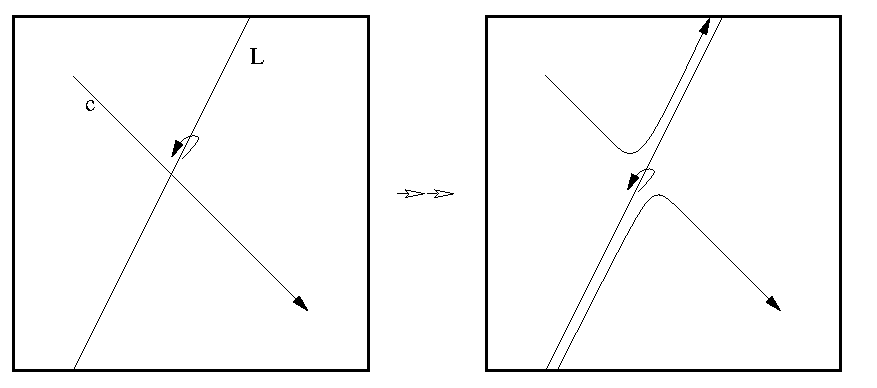
\includegraphics[width=0.85\linewidth]{figures/fig1.pdf}
  \caption{Dehn 扭转 $\tau_L$ 对测试曲线 $c$ 的作用。（原文 Figure 1，第 18 页）}
  \label{fig:dehn-twist}
\end{figure}

\subsection{分次辛几何}
\label{subsec:graded-sympl}

下面把上述想法推广，以纳入 "分次"。这些材料都可在 [18] 中找到。

先回忆：任何流形 $M$ 上都有自然的纤维丛 $\pi: \mathrm{Gr}(n,M)\to M$，其纤维为 $\mathrm{Gr}(n,T_xM)$。若 $M$ 是 $2n$ 维辛流形，则可取拉格朗日子空间构成的子丛 $\mathrm{LGr}(M)\subset\mathrm{Gr}(n,M)$，称为 $M$ 的\emph{拉格朗日 Grassmann 流形}。对任意拉格朗日子流形 $L\subset M$，存在自然截面 $s_L: L\to\mathrm{LGr}(M)$（由 $s_L(x)=T_xL$ 给出）。若 $\phi: M\to M$ 是辛同胚，则有覆盖 $\phi$ 的映射 $\phi_*: \mathrm{LGr}(M)\to\mathrm{LGr}(M)$，由 $\phi_*(x,L_x)=(\phi(x),D\phi L_x)$ 给出。对任意拉格朗日子流形 $L$，它满足 $\phi_* s_L = s_{\phi(L)}\phi|_L$。

回忆：对相当好的空间 $X$ 与阿贝尔群 $A$，$X$ 的 $A$-覆盖（即带有 $A$ 的连续、逐纤维传递且忠实作用的覆盖空间）由 $H^1(X,A)$ 分类。

\begin{definition*}
设 $(M,\omega)$ 是辛流形。$M$ 的 \emph{Maslov 覆盖}（Maslov cover）是指 $\mathrm{LGr}(M)$ 的一个 $\ZZ$-覆盖 $\cL$，具有如下性质：若 $c\in H^1(\mathrm{LGr}(M),\ZZ)$ 分类 $\cL$，$x\in M$，而 $i_x: \mathrm{LGr}(T_xM)\to\mathrm{LGr}(M)$ 表示纤维的包含，则
\[
  i_x^*(c) = s_{T_xM}.
\]
\end{definition*}

回忆 $s_{T_xM}$ 表示 $\mathrm{LGr}(T_xM)$ 的 Maslov 类，它是 $H^1(\mathrm{LGr}(T_xM),\ZZ)$ 的典范生成元。由于 $\pi_1(\mathrm{LGr}(T_xM))=\ZZ$，特别可知 $\cL$ 是 $M$ 上的纤维丛，其纤维是 $\mathrm{LGr}(T_xM)$ 的万有覆盖。可以证明：Maslov 覆盖存在当且仅当 $2c_1(M)=0$（其中 $c_1(M)$ 表示切丛的第一陈类）。事实上，取 $M$ 上相容的近复结构，记 $\Delta_M=\Delta(M,\omega,I):=\Lambda^n(TM,\CC)^{\otimes 2}$。则 $M$ 的 Maslov 覆盖与 $\Delta_M$ 的平凡化的同伦类一一对应（特别地，它们构成 $H^1(M,\ZZ)$ 上的仿射空间），见 [18, lemma 2.2] 及其前面的讨论。

% [Tutor Note: 这是全节最容易被跳过的论证，实质如下。$\Delta_M=\Lambda^n(TM,\mathbb C)^{\otimes 2}$ 是复线丛，其单位圆丛 $S(\Delta_M)\to M$ 是 $S^1$-丛，第一陈类为 $c_1(\Delta_M)=2c_1(M)$。而 Maslov 覆盖 $\cL$ 在每个纤维上正是 $\mathrm{LGr}(T_xM)$ 的万有覆盖，这等价于把 $S(\Delta_M)$ 的纤维方向 "展开" 成 $\mathbb R$；因此 $\cL$ 与 $S(\Delta_M)$ 的平凡化是同一件事。$S^1$-丛可平凡化 $\iff$ 其第一陈类为零，即 $2c_1(M)=0$；平凡化的同伦类构成 $H^1(M,\mathbb Z)$ 的仿射空间（两个平凡化的比是 $M\to S^1$ 的映射类）。]

% [Tutor Note: 定义中的条件 $i_x^*(c)=s_{T_xM}$ 必须盯紧：$c$ 是 $M$ 上 $\mathrm{LGr}(M)$ 的 $H^1$ 类，把它拉回到纤维 $i_x$ 上，必须恰好是纤维的典范生成元（而不是它的某个整数倍）。若写成 $i_x^*(c)=n\,s_{T_xM}$（$n\ne 1$），得到的就不是 Maslov 覆盖，$\mathbb Z$-分次会整体缩并，Floer 复形的次数会出错。]

给拉格朗日子流形分次的主要理由如下：设 $(L_1,t_1)$ 与 $(L_2,t_2)$ 是分次拉格朗日子流形，$x\in L_1\cap L_2$。在 $\cL_x$ 中取从 $t_1(x)$ 到 $t_2(x)$ 的道路 $\gamma$。由于 $\cL_x$ 是 $\mathrm{LGr}(T_xM)$ 的万有覆盖，该道路在同伦意义下唯一。因此
\[
  \mu_x(L_1,L_2) := \mu(\pi\gamma)
\]
（右端表示定理 \ref{thm:4.1} 中道路的 Maslov 指标）是良定义的，称为 $x$ 的 \emph{Maslov 指标}。

% [Tutor Note: 这里 $\pi$ 指万有覆盖投影 $\cL_x\to\mathrm{LGr}(T_xM)$。注意 $\cL_x$ 是 Maslov 覆盖在 $x$ 处的纤维，$t_i(x)$ 是该纤维中的点，其投影才是拉格朗日子空间 $T_xL_i$；于是 $\pi\gamma$ 是 $\mathrm{LGr}(T_xM)$ 中从 $T_xL_1$ 到 $T_xL_2$ 的道路，$\mu(\pi\gamma)$ 正是定理 \ref{thm:4.1} 的路径 Maslov 指标。这个整数就是交点 $x$ 的 $\mathbb Z$-次数，它可以是负数——这正是分次框架比 $\mathbb Z/2$ 框架强的地方。]

称辛流形 $(M,\omega)$ 连同一个 Maslov 覆盖 $\cL$ 的选择为\emph{分次流形}（graded manifold）。所谓\emph{分次拉格朗日子流形}（graded Lagrangian），是指拉格朗日子流形 $L$ 连同 $s_L$ 的提升 $t_L: L\to\cL$。所谓\emph{分次辛同胚} $\phi: (M,\omega_M,\cL_M)\to(N,\omega_N,\cL_N)$，是指辛同胚 $\phi: M\to N$，连同覆盖 $\phi_*: \mathrm{LGr}(M)\to\mathrm{LGr}(N)$ 的 $\ZZ$-等变提升 $\phi_*: \cL_M\to\cL_N$。

分次辛同胚可按自然方式复合，记 $\Sym^{gr}(M)$ 为 $M$ 的分次辛同胚群。其中有一个中心子群 $\{\mathbf 1[n]\mid n\in\ZZ\}\simeq\ZZ$，$\mathbf 1[n]$ 由 $\phi=\mathbf 1$、$\phi_*(x)=x+n$ 给出（用覆盖上的 $\ZZ$-作用）。对任意分次自同构 $\phi$，记 $\phi[n]:=\mathbf 1[n]\phi=\phi\mathbf 1[n]$。注意 $\Sym^{gr}(M)$ 自然地作用在分次拉格朗日子流形的集合上。若 $L$ 是分次拉格朗日子流形，则用 $L[n]$ 记分次拉格朗日子流形 $\mathbf 1[n](L)$。此外，若 $\phi_1$ 与 $\phi_2$ 由辛同伦连接，则 $\phi_1$ 的分次诱导 $\phi_2$ 的分次。

% [Tutor Note: 这里的 $\mathbb Z$-作用必须盯紧符号：$\mathbf 1[n]$ 把覆盖的纤维坐标加 $n$，而 $L[n]:=\mathbf 1[n](L)$ 使所有交点的次数整体减去 $n$，即 $\mu_x(L[n],L')=\mu_x(L,L')-n$。理由：把 $t_1(x)$ 换成 $t_1(x)+n$ 后，覆盖中从新起点到 $t_2(x)$ 的道路投影到 $\mathrm{LGr}$ 后与原来的道路相差一个环路，该环路的 Maslov 指标正是 $-n$。$[1]$ 就是 Floer 复形的平移函子；若这个符号取反，$m_1^2=0$ 与 $m_2$ 的 Koszul 符号都会错。又因为 $\mathbf 1[n]$ 是中心元，$\phi[n]=\mathbf 1[n]\phi=\phi\mathbf 1[n]$ 才无歧义。]

% [Tutor Note: "若 $\phi_1$ 与 $\phi_2$ 由辛同伦连接，则 $\phi_1$ 的分次诱导 $\phi_2$ 的分次" 的论证被省略了：$\phi$ 的分次是 $\phi_*:\mathrm{LGr}(M)\to\mathrm{LGr}(M)$ 的提升的同伦类；辛同伦给出 $\phi_{1*}$ 与 $\phi_{2*}$ 之间的同伦，而同伦的映射其提升之间存在典范对应。这也说明分次在 $\Sym^{gr}(M)$ 上只依赖于连通分支。]

可以用上同调描述哪些辛同胚与拉格朗日子流形可分级、以及有多少种分次，见 [18, lemmas 2.3 and 2.4]。我们不需要这些。

\subsubsection{更显式的描述}
\label{subsec:graded-explicit}

设 $(M,\omega)$ 是辛流形，取定相容近复结构。设有非零截面 $\Omega\in\Delta_M$，满足 $|\Omega|\equiv 1$（即 $\Delta$ 的一个平凡化）。令
\[
  \cL_\Omega = \mathrm{LGr}(M)\times_{s,\Delta,c}\RR = \{(L,r)\mid s(L)=c(r)\}.
\]
这里 $\RR$ 表示平凡丛，$c: \RR\to S(\Delta)$ 是由 $\Omega$ 诱导的自然覆盖，而 $s: \mathrm{LGr}(M)\to\Delta$ 是自然映射。这是一个 Maslov 覆盖；可以证明事实上所有 Maslov 覆盖都这样得到。

% [Tutor Note: 这一步的实质是两个 $\mathbb Z$-覆盖之差：任取 Maslov 覆盖 $\cL$，它与 $\cL_\Omega$ 的差别是一个沿纤维方向为常数的连续函数，因而来自 $M$ 上的映射 $M\to S^1$，即 $H^1(M,\mathbb Z)$ 中的一个类。这就同时给出 "所有 Maslov 覆盖都如此" 与 "$H^1(M,\mathbb Z)$-仿射结构" 两条结论。]

现设 $L$ 是 $M$ 的拉格朗日子流形，$t_L: L\to\cL_\Omega$ 是分次。则可写 $t_L(x)=(s(s_L(x)),\tilde s_L(x))$，其中 $\tilde s_L: L\to\RR$ 是某个函数。此时
\[
  e^{2\pi i\tilde s_L(x)}\Omega(x) = s(s_L(x)),
\]
而这样的（连续）函数与 $L$ 的分次一一对应。

类似地，若 $\phi: M\to M$ 是辛自同构，则给 $\phi$ 一个分次，等同于给一个连续函数 $\tilde s_\phi: \mathrm{LGr}(M)\to\RR$，使得对任意 $x\in M$ 与 $L\in\mathrm{LGr}(M)_x$ 有
\[
  s(D\phi(L)) = e^{2\pi i\tilde s_\phi(L)}\Omega(x).
\]

% [Tutor Note: 上式两边严格说应在同一点取值：$s(D\phi(L))$ 落在 $\Delta$ 的 $\phi(x)$ 纤维上，而右端写的是 $\Omega(x)$。按原文的约定（$\Omega$ 是整体平凡化，$|\Omega|\equiv1$ 故可用它把各纤维的相位统一到 $\mathbb C$），这种写法可以接受；但若改用 $x$ 与 $\phi(x)$ 不同处的 $\Omega$，$\tilde s_\phi$ 会多出 $\phi$ 的相位项。核对 [18] 时请注意这一约定。]

现设 $(\phi,\tilde s_\phi)$ 与 $(\psi,\tilde s_\psi)$ 是分次辛同胚，而 $(L,\tilde s_L)$ 是分次拉格朗日子流形。则容易验证
\begin{align*}
  \tilde s_{\psi\phi} &= \tilde s_\phi + \tilde s_\psi\circ D\phi,\\
  \tilde s_{\phi(L)} &= \tilde s_L\circ\phi^{-1} + \tilde s_\phi\circ s_L\circ\phi^{-1}.
\end{align*}

% [Tutor Note: 这两式是 "分次" 的复合律，符号极容易错。第一式：先做 $\phi$ 再做 $\psi$，相位要加上 $\tilde s_\psi$ 在 $D\phi$ 处的值（因为 $\psi$ 的相位是在切空间上评价的）。第二式右端的 $\phi^{-1}$ 出现两次，是因为左端 $\tilde s_{\phi(L)}$ 是定义在 $\phi(L)$ 上的函数；若把它看成定义在 $L$ 上的函数（即比较 $\tilde s_{\phi(L)}\circ\phi$），就得到 $\tilde s_L+\tilde s_\phi\circ s_L$ 这种更常见的写法。两种写法差一个拉回，不是笔误。]

\subsubsection{例：平坦环面}
\label{subsec:maslov}

现在考虑环面 $T=\CC/\ZZ^2$。它带有自然的（常值）辛形式与全纯结构。我们得到 $\Delta_T$ 的一个平凡化 $\Omega=\partial/\partial z^{\otimes 2}$。在同伦意义下，其余所有平凡化都有形式 $\Omega_{m,n}(x,y)=e^{2\pi i(mx+ny)}\Omega$。于是对 $m,n\in\ZZ$ 得到相应的 Maslov 覆盖 $\cL_{m,n}$；由上面的讨论，这给出了全部 Maslov 覆盖。

% [Tutor Note: 记号存疑：$\Delta_M$ 按定义是 $\Lambda^n(TM,\mathbb C)^{\otimes 2}$，即切丛的最高外幂的平方，而原文写的 $\Omega=\partial/\partial z^{\otimes 2}$ 用的是切向量（$\partial_z$）而非余切向量（$dz$）。在 Hermite 度量下二者可（共轭线性地）等同，故不一定是笔误；但与 [18] 对照时须统一约定，否则 $s(L)$ 与 $e^{2\pi i\tilde s}\Omega$ 的相对相位会差一个共轭。另注意这里的 $z$ 是复坐标，$x,y$ 是 $T$ 上的实坐标，$\Omega_{m,n}$ 的相位因子 $e^{2\pi i(mx+ny)}$ 正是 $H^1(T,\mathbb Z)$ 的仿射参数。]

现在容易验证：相对于与全纯平凡化 $\Omega$ 对应的覆盖 $\cL=\cL_{0,0}$，一个拉格朗日圆周可分级当且仅当它不是可缩的。相反，若 $(m,n)\ne(0,0)$，则可缩圆周仍然不可分级，但此时总还存在进一步的（非可缩的）不可分级圆周。因此全纯平凡化是 Maslov 覆盖的一个自然选择。此外，对这个 Maslov 覆盖的选取，$T$ 的任意辛自同构都可分级。（所有这些陈述都是容易的练习。）

% [Tutor Note: "easily checked" 的实际内容是三步：(i) 可分级 $\iff$ $s_L$ 可提升到 $\cL$ $\iff$ 沿 $L$ 绕一周 Maslov 指标的变化为零（即 $s_L^*(c)=0\in H^1(L,\mathbb Z)$）；(ii) 对 $\mathbb C/\mathbb Z^2$ 与全纯平凡化逐同调类计算该指标，得到 "可缩圆周不可分级、非可缩圆周可分级"；(iii) 换用 $\cL_{m,n}$ 后，$c$ 类被乘以相位 $e^{2\pi i(mx+ny)}$，可分级圆周的集合随之改变，并且总有额外的非可缩不可分级圆周出现。这条练习的关键结论是：Maslov 覆盖的选择会改变 A-模型的分次数据，故镜像对称的陈述必须先固定它。]

% [Tutor Note: 为什么全纯平凡化是 "自然" 的？因为它由 $T$ 的复结构直接给出，因而与 B-模型侧的代数结构（$\mathcal O_T$ 与全纯坐标）典范相容；HMS 中的分次对应正是在这一选择下才逐次相符。换成 $\cL_{m,n}$ 相当于对 A-模型作一次 "平坦的 $\mathbb Z$-平移 twisting"，物理上对应一个不改变拓扑、但改变分次数据的背景场。]

\subsection{辛曲面的 Fukaya 范畴}
\label{subsec:fuk-surface}

下面描述紧辛曲面（带 Maslov 覆盖的选择）的 Fukaya 范畴，即环面 $T$（带某种辛形式与 Maslov 覆盖的选择）。密切相关的讨论见 [1]，也见我们的主要参考 [19]。

% [Tutor Note: 原文此处脱字："the Fukaya category a compact symplectic surface" 应为 "the Fukaya category of a compact symplectic surface"，译文按文意补出 "的"。]

设 $L_1,L_2,\dots,L_n$ 是 $T$ 中的分次拉格朗日圆周（即紧连通拉格朗日子空间，并带分次的选择），且两两横截。则对 $i\ne j$，集合 $L_i\cap L_j$ 有限。用 $\Lambda_t$ 记形式幂级数 $\sum_{n>0}a_n t^{b_n}$ 的域，其中系数 $a_n\in\CC$，实指数 $b_n\in\RR$ 当 $n\to\infty$ 时趋于无穷。于是构成 \emph{Floer 链空间}
\[
  CF^*(L_i,L_j) = \bigoplus_{x\in L_i\cap L_j} [x]\Lambda_t,
\]
其中 $[x]$ 是次数为 $\mu_x(L_i,L_j)$ 的形式生成元。

% [Tutor Note: 系数域必须用实指数的形式幂级数 $\Lambda_t$（Novikov 域），而不是普通多项式：多边形计数一般有无穷多个（面积可以趋于无穷），$A_\infty$ 关系中每个系数都是无穷和，需要一个既允许无穷和、又保持 "最低次项"（按面积过滤）有限的系数域。实指数 $b_n\to\infty$ 保证在任一有界面积区间内只有有限项，这是 Gromov 紧性在代数侧的对应物。]

下面说明如何定义运算
\[
  m_n : CF^*(L_n,L_{n-1})\otimes\cdots\otimes CF^*(L_1,L_2) \longrightarrow CF^*(L_1,L_n),
\]
使得只要 $A_\infty$-关系有意义就成立。具体地，令
\[
  m_n(p_{n-1},\dots,p_1) = \sum_{q\in L_1\cap L_n} C(q;p_1,\dots,p_{n-1})[q].
\]
这里 $p_i\in L_i\cap L_{i+1}$。下面解释如何计算系数 $C(q;p_1,\dots,p_{n-1})$。

% [Tutor Note: 原文疑误：$m_n$ 的定义域写成 $CF^*(L_n,L_{n-1})\otimes\cdots\otimes CF^*(L_1,L_2)$，但按紧接着的 $p_i\in L_i\cap L_{i+1}$ 以及定理 \ref{thm:4.2} 第 (1) 条（$\Hom(L_{n-1},L_n)\otimes\cdots\otimes\Hom(L_1,L_2)\to\Hom(L_1,L_n)$），第一个因子应为 $CF^*(L_{n-1},L_n)$。两处不自洽，译文保留原文定义式，实际计算以定理 \ref{thm:4.2} 的写法为准。]

用 $D_n$ 记单位圆盘，其边界上依次有标号点 $P_1,P_2,\dots,P_{n-1}$ 与 $Q$（按此顺序）。用 $\gamma_i$ 记终止于 $P_i$ 的边界弧段。用 $\mathcal{M}(q;p_1,\dots,p_{n-1})$ 记浸入多边形 $u: D_n\to X$ 的等价类集合，满足：(1) $u$ 保定向，且在 $P_i$ 与 $Q$ 之外是嵌入；(2) $u$ 在 $P_i$ 与 $Q$ 处有凸角；(3) $u(P_i)=p_i$ 且 $u(Q)=q$；(4) $u(\gamma_i)\subset L_i$。两个嵌入多边形若相差 $D_n$ 的一个微分同胚，则视为等价。

% [Tutor Note: 原文疑误：此处写 $u:D_n\to X$，但本节只讨论环面 $T$，前面的记号也一直用 $T$，应为 $u:D_n\to T$。译文保留原文的 $X$ 以便对照。]

然后令
\[
  C(q;p_1,\dots,p_{n-1}) = \sum_{u\in\mathcal{M}(q;p_1,\dots,p_{n-1})} \pm\, t^{\int_{D_n} u^*\omega}.
\]
这里 $\pm$ 表示一个我们不打算解释的符号\footnote{我们不需要这个符号，只需要存在某种符号规则使下面的定理成立。}。

% [Tutor Note: 脚注 "只需要存在符号规则" 是轻描淡写：一般情形下符号来自拉格朗日的相对 spin（或 Pin）结构与定向数据，且必须精密到使 $m_1^2=0$ 与 $A_\infty$ 结合律成立；在二维情形这些都可显式选出。原文略去符号不影响定理 \ref{thm:4.2} 的陈述，但若要真正算 $m_2$ 的显式公式（§6 的计数），符号约定必须与 [19] 对齐，否则 $A_\infty$ 关系的验证会差号。]

遗憾的是，这里没有篇幅解释为什么这样得到满足 $A_\infty$-关系的映射。下面的定理汇总了我们将要用到的 Fukaya 范畴的性质。

\begin{theorem}\label{thm:4.2}
设 $(T,\omega,\cL)$ 是分次流形，其中 $T$ 是环面。\emph{Fukaya 范畴} $\Fuk(T)$ 以分次拉格朗日子流形 $(L,t_L)$ 为对象。此外：
\begin{enumerate}[leftmargin=1.8em, itemsep=2pt, topsep=2pt]
  \item 若 $L_1,L_2\in\Fuk(T)$ 横截，则 $\Hom_{\Fuk(T)}(L_1,L_2)=CF^*(L_1,L_2)$。若 $L_1,\dots,L_n$ 横截，则
  \[
    m_n^{\Fuk(T)}: \Hom(L_{n-1},L_n)\otimes\cdots\otimes\Hom(L_1,L_2) \longrightarrow \Hom(L_1,L_n)
  \]
  就是上面构造的映射。
  \item 存在 $\Sym^{gr}(T)$ 在 $\Fuk(T)$ 上的作用。在对象上，它就是先前构造的作用。此外，若 $\phi$ 是哈密顿同伦于恒等的分次辛同胚，则它在 $\Fuk(T)$ 上的作用拟同构于恒等函子。
  \item 若 $L$ 是拉格朗日圆周，$\tilde\tau_L$ 表示 $L$ 上带标准分次的辛 Dehn 扭转（symplectic Dehn twist），而 $L'\in\Fuk(T)$，则
  \[
    T_L(L') \simeq \tilde\tau_L(L').
  \]
  这里 $T_L$ 表示第 \ref{subsec:ainf-twisting} 节中的代数扭变函子（twist functor）。
\end{enumerate}
\end{theorem}

% [Tutor Note: 第 (2) 条里 "拟同构于恒等函子" 不能加强为 "等于"：哈密顿同伦只保证作用在对象上同构、在态射上差一个同伦，且这个同构本身依赖同伦的选取；这正是 A-模型侧 "规范等价" 的含义。与第 (3) 条合起来看，$\Sym^{gr}(T)$ 的作用把几何的自同构变成范畴的自等价，而哈密顿同伦类对应的是 "平凡" 的那部分。]

% [Tutor Note: 第 (3) 条是本文的核心对应之一：代数侧沿球状对象 $L$ 的扭变函子 $T_L$（在导出范畴中的标准公式是 "evaluation 的锥"）与辛侧沿 $L$ 的 Dehn 扭转 $\tilde\tau_L$ 在对象上一致。几何图像：Dehn 扭转把穿过 $L$ 的测试曲线 $c$ 在一侧剪开再粘回（图 \ref{fig:dehn-twist}），对交点计数的效果等同于把 $c$ 卷过 $L$；$T_L$ 的锥公式正是这一操作的代数化。注意必须用带 "标准分次" 的 $\tilde\tau_L$：否则 $\mathbb Z$-次数会错位，$\tilde\tau_L(L')$ 与 $T_L(L')$ 只能同构到某个平移 $[n]$ 为止，定理就不成立。]
     % §3 The enhanced derived category / §4 The Fukaya category
% ============================================================
%  sec05_06a.tex
%  §5 Hochschild 上同调与 $A_\infty$-结构的分类（原文 pp.21–24）
%  §6 $\Lambda_t$ 上椭圆曲线的镜像对称，含 6.1 代数 $Q$
%     （原文 pp.24–28，止于 p.29 “6.2. The derived category of an elliptic curve” 标题之前）
%  原文：Homological Mirror Symmetry for Elliptic Curves（2013-04-25）
%  说明：文献引用沿用原文编号 [n]；跨节引用使用 GUIDE §6.5 登记的标签 key。
% ============================================================

\section{\texorpdfstring{Hochschild 上同调与 $A_\infty$-结构的分类}{Hochschild 上同调与 A∞-结构的分类}}\label{sec:hoch}

\begin{keytakeaways}
  \item \textbf{数学工具}：把 $A_\infty$-代数重新表述为约化余张量余代数 $\bar T(SA)$ 上次数为一的余微分 $b$；$A_\infty$-方程恰是 $b^2=0$，$A_\infty$-态射恰是与 $b$ 交换的余代数态射。
  \item \textbf{代数机制}：Hochschild 复形 $CC^{m,n}=\Hom_k(A^{\otimes m},SA(n))$ 上的微分是超 Lie 括号 $D=[b,\cdot]$，因此 $HH^{m,n}(A)\simeq\Ext^m_{A\otimes A^{op}}(A,A(n))$。
  \item \textbf{核心结论}：延拓给定乘法的 $A_\infty$-结构，其规范等价类的自由度逐阶由 $HH^{d,2-d}(A)$ 控制；若这些群除 $d=R$ 外全为零、在 $d=R$ 处一维，则至多差一个障碍类（定理 \ref{thm:5.3}）。
  \item \textbf{几何图像}：$HH^{\bullet,2-\bullet}$ 上有一个自然的重标度作用 $\epsilon$，它把障碍类按 $\tilde\epsilon^{d-2}$ 缩放；下一节将看到，这正是镜像映射把 $a_4,a_6$ 与 Weierstrass 系数 $a,b$ 对齐的代数根源。
\end{keytakeaways}

本节说明如何用 Hochschild 上同调对极小的 $A_\infty$-结构进行分类。第一小节用分次余代数重新解释 $A_\infty$-代数，这部分材料在 [9, 3.6] 中有最简洁的总结。第二小节定义 Hochschild 上同调并说明它的一些性质，其中大部分材料可在 [5] 以及 [19, 第 3 节] 中找到。

\subsection{\texorpdfstring{$A_\infty$-结构与余代数余微分}{A∞-结构与余代数余微分}}\label{subsec:coalgebra}

我们先以一种不那么“就事论事”的方式重新解释 $A_\infty$-方程。为此回忆：\emph{分次余代数}是分次向量空间 $V$ 连同余乘法 $\Delta:V\to V\otimes V$，满足某种与代数定义相对偶的“结合性条件”；\emph{次数为 $d$ 的余导子}是 $\Hom(V,V(d))$ 中的一个元素，满足某种与代数上导子定义相对偶的关系；最后，余代数态射的概念同样按显然的方式定义。我们指出：$\Delta$ 与余代数态射都自动是次数为零的。

% [Tutor Note: 此处“对偶”不是把箭头简单地反向：分次情形下取对偶 $V\mapsto V^*=\bigoplus_n\Hom(V_n,k)$ 会翻转次数并引入 Koszul 符号，所以“与结合性相对偶的条件”是一个带符号的多重线性恒等式，而不是把 $\mu\circ(\mu\otimes1)=\mu\circ(1\otimes\mu)$ 的字面转写。本节让 $\Delta$ 与余代数态射自动为次数零，全部符号都推迟到 $A_\infty$ 方程、Hochschild 微分与 Lie 括号里出现，这是最容易在读第二遍时搞混的地方。]

我们主要的余代数例子如下。设 $V$ 是分次向量空间，则 $V$ 上的\emph{约化余张量余代数}（reduced cotensor coalgebra）为
\[
\bar TV=\bigoplus_{n>0}V^{\otimes n}.
\]
以下把 $v_1\otimes\cdots\otimes v_n$ 记作 $v_1\ldots v_n$，并给 $\bar TV$ 赋分次 $|v_1\ldots v_n|=|v_1|+\cdots+|v_n|$。记 $\bar T^nV=V^{\otimes n}$，视之为 $\bar TV$ 的子空间。余乘法由
\[
\Delta(v_1\ldots v_n)=\sum_{k=1}^{n}(v_1\ldots v_k)\otimes(v_{k+1}\ldots v_n)
\]
定义。

% [Tutor Note: $\Delta$ 的公式里 $k$ 遍历所有可能的切分位置；$k=n$ 时右侧第二因子是空词。约化余张量余代数通常把空词当作单位元 $1$ 并令 $\Delta(1)=0$，原文未明说但后文所有公式都不涉及这一项；若在别的文献中看到 $\Delta(v_1)=v_1\otimes1+1\otimes v_1$，那是非约化版本，切勿与本节的 $\Delta$ 混用。]

这个余代数在许多方面表现得“对偶于”通常的张量代数。它的性质总结为下述命题，其证明是一个容易的练习。

\begin{proposition}\label{prop:5.1}
设 $V$ 与 $W$ 是分次向量空间。记 $\pi:\bar TV\to V$ 为到第一个直和项的投影。对任意分次向量空间 $U$ 与线性映射 $f:U\to\bar TV$，把 $\pi_*(f)$ 记作复合 $\pi\circ f$。
\begin{enumerate}
  \item 映射
  \[
  \{\text{$\bar TV\to\bar TV$ 上次数为 $d$ 的余导子}\}\xrightarrow{\ \pi_*\ }\Hom_k(\bar TV,V(d))=\prod_{n>0}\Hom_k(V^{\otimes n},V(d))
  \]
  是双射；其逆映射把 $(b_i)\in\prod_{n>0}\Hom_k(V^{\otimes n},V(d))$ 送到 $b$，其中
  \[
  b|_{\bar T^nV}=\sum_{a+b+c=n}1^{\otimes a}\otimes b_i\otimes 1^{\otimes b}.
  \]
  \item 映射
  \[
  \{\text{$\bar TV\to\bar TW$ 的余代数态射}\}\xrightarrow{\ \pi_*\ }\Hom_k(\bar TV,W)=\prod_{n>0}\Hom_k(V^{\otimes n},W)
  \]
  是双射；其逆映射把 $(f_i)\in\prod_{n>0}\Hom_k(V^{\otimes n},W)$ 送到 $f$，其中
  \[
  f|_{\bar T^nV}=\sum_{r,\ a_1+\cdots+a_r=n}f_{a_1}\otimes\cdots\otimes f_{a_r}.
  \]
\end{enumerate}
\end{proposition}

% [Tutor Note: 命题 5.1 的“容易练习”实质上要做两件事：(i) 用余张量余代数的泛性质验证“余导子/余代数态射”与“分量族 $(b_i)$/$(f_i)$”一一对应；(ii) 验证由所示公式拼出的 $b$ 确实满足余导子条件 $\Delta b=(b\otimes1+1\otimes b)\Delta$。关键机制是：$\Delta$ 把长度 $n$ 的词拆成长度 $k$ 与 $n-k$ 的两段，而 $b$ 只作用在其中一段上，故求和遍历该连续子词的全部位置。]

% [Tutor Note: 原文疑误：$b|_{\bar T^nV}=\sum_{a+b+c=n}1^{\otimes a}\otimes b_i\otimes1^{\otimes b}$ 的指标不自洽——和式用了 $a,b,c$ 三个指标，但右侧只出现 $1^{\otimes a}$、$b_i$、$1^{\otimes b}$，$c$ 与 $i$ 都没有被和式约束。按标准公式应为 $\sum_{a+i+c=n}1^{\otimes a}\otimes b_i\otimes1^{\otimes c}$（即分量 $b_i$ 作用在长度 $i$ 的连续子词上，左右各固定 $a$、$c$ 个因子）。译文保留原文写法，使用时请按标准公式理解。]

以下我们也把 $\pi_*(f)$ 在 $\bar T^iV$ 上的限制记作 $\pi_*(f)_i\in\Hom(V^{\otimes i},V(d))$。

我们引入这些余代数的主要原因是它们与 $A_\infty$-代数的联系。下述命题同样只是把定义写开的一个容易练习。对分次向量空间 $V$，记 $SV$ 为分次向量空间 $V(1)$，$s:V\to SV$ 为自然的（次数 $-1$ 的）\emph{平移映射}。

\begin{proposition}\label{prop:5.2}
\begin{enumerate}
  \item 设 $A$ 是分次向量空间。$A$ 上的 $A_\infty$-结构与 $\bar T(SA)$ 上次数为一的余微分是同一回事。确切地说，给定余微分 $(b_i)\in\prod_{n>0}\Hom_k((SA)^{\otimes n},SA(1))$，由
  \[
  m_i=s^{-1}b_is^{\otimes i}\in\Hom_k(A^{\otimes n},A(2-i))
  \]
  给出的映射 $m_i$ 定义 $A_\infty$-结构，当且仅当 $b^2=0$。
  \item 设 $A$ 与 $B$ 是 $A_\infty$-代数，相应的余导子为 $b_A$ 与 $b_B$。则 $A_\infty$-态射 $A\to B$ 与满足 $fb_A=b_Bf$ 的余代数态射 $f:\bar T(SA)\to\bar T(SB)$ 是同一回事。
\end{enumerate}
\end{proposition}

% [Tutor Note: 符号易错：$s$ 的次数为 $-1$，故 $\deg s^{-1}=+1$、$\deg s^{\otimes i}=-i$；又 $\deg b_i=1$，于是 $\deg m_i=(+1)+1-i=2-i$，这正是 $A_\infty$-结构映射 $m_i:A^{\otimes i}\to A(2-i)$ 的标准次数（$m_2$ 次数 $0$，$m_3$ 次数 $-1$，依此类推）。若把 $s$ 误当成次数 $+1$，所有次数都会整体平移，$A_\infty$ 方程的符号也会随之改变。]

% [Tutor Note: 原文疑误：命题 5.2 中 $m_i=s^{-1}b_is^{\otimes i}$ 的陪域写作 $\Hom_k(A^{\otimes n},A(2-i))$，但 $m_i$ 取 $i$ 个输入，应为 $\Hom_k(A^{\otimes i},A(2-i))$。这一句里乘积指标 $n$ 与分量指标 $i$ 混用了（$(b_i)\in\prod_{n>0}\Hom_k((SA)^{\otimes n},SA(1))$ 亦如此）。译文保留原文写法。]

本节余下部分固定一个分次向量空间 $A$。记
\[
C^{m,n}=\Hom_k((SA)^{\otimes m},SA(n)),\qquad C^n=\Hom_k(\bar T(SA),SA(n))\simeq\prod_r C^{r,n}.
\]
上述命题允许我们把 $C^n$ 看作 $\bar T(SA)$ 上余导子的空间。对分次余导子 $b_1$ 与 $b_2$，记
\[
[b_1,b_2]=b_1b_2-(-1)^{|b_1||b_2|}b_2b_1,
\]
并称之为（超）\emph{Lie 括号}。易于验证它满足\emph{分次 Jacobi 恒等式}
\begin{equation}\label{eq:hoch-jacobi}
(-1)^{|x||z|}[x,[y,z]]+(-1)^{|y||x|}[y,[z,x]]+(-1)^{|z||y|}[z,[x,y]]=0 .
\end{equation}
还可验证 Lie 括号与分次相容，即 $[C^{m,n},C^{p,q}]\subset C^{m+p-1,n+q}$。

% [Tutor Note: 式 \eqref{eq:hoch-jacobi} 的 Koszul 符号极易抄错：三项的符号 $(-1)^{|x||z|}$、$(-1)^{|y||x|}$、$(-1)^{|z||y|}$ 恰好是把对应的第一个元素移到最左端所需的符号，因此三项是同一个式子的循环置换。注意本文的括号是 $[b_1,b_2]=b_1b_2-(-1)^{|b_1||b_2|}b_2b_1$；当 $b_1,b_2$ 均为奇（例如两个次数一的余导子）时它就是反对易子 $b_1b_2+b_2b_1$。]

\subsection{Hochschild 上同调}\label{subsec:hoch-cohomology}

\begin{definition*}
设 $A$ 是分次向量空间。记
\[
CC^{m,n}=CC^{m,n}(A)=\Hom_k(A^{\otimes m},SA(n))
\]
为 Hochschild 链空间（Hochschild chain spaces），并记 $CC^n=\prod_{p+q=n}CC^{p,q}$。
\end{definition*}

借助 $s:A\to SA$，有同构（作为分次向量空间）$CC^{m,n}\simeq C^{m,m+n-1}$ 与 $CC^n\simeq C^n$。这把超 Lie 结构移植到 $CC^{\bullet,\bullet}$ 上。

% [Tutor Note: 这两个同构是由 $s$ 诱导的：把 $\Hom_k(A^{\otimes m},SA(n))$ 中的元素 $x$ 的两侧分别乘以 $s$ 与 $(s^{-1})^{\otimes m}$，即 $x\mapsto sx(s^{-1})^{\otimes m}$，就得到 $\Hom_k((SA)^{\otimes m},SA(\cdot))$ 中的元素，第二个指标恰好差 $m-1$。验证时把 $|s|=-1$ 逐项代入，是检查上述“$\simeq$”是否抄对的唯一稳妥办法。]

现设 $A$ 是分次代数。回忆这只是 $A_\infty$-代数的特例：$m_i=0$（$i\neq2$），因此命题 \ref{prop:5.2} 给出次数为一的余微分 $b\in CC^{2,0}$。对 $x\in CC^{m,n}$，定义 \emph{Hochschild 微分} $D(x)=[b,x]$。有
\[
D(CC^{m,n})\simeq[b,C^{m,m+n-1}]\subset C^{m+1,m+n}\simeq CC^{m+1,n}.
\]
分次 Jacobi 恒等式 \eqref{eq:hoch-jacobi} 说明 $D$ 确实是微分，且满足\emph{分次 Leibniz 法则}。

% [Tutor Note: 原文此处把 "Leibniz" 误排为 "Leinbniz"（p.23），译文按正确拼写处理。]

% [Tutor Note: 注意 $D=[b,\cdot]$ 是双分次 $(1,0)$ 的：它把第一个指标（输入因子个数，对应 $\Ext$ 的次数）加一，而第二个指标 $n$（内部分次，对应系数平移 $A(n)$）保持不变。因此对每个固定的 $n$，$CC^{\bullet,n}$ 各自是一个复形——上同调 $HH^{m,n}$ 的双分次结构即由此而来，读后面 $\Ext^m_{A\otimes A^{op}}(A,A(n))$ 时不要漏掉这个 $n$。]

\begin{definition*}
$A$ 的\emph{双分次 Hochschild 上同调}（bigraded Hochschild cohomology）是 $CC^{\bullet,n}(A)$ 关于 $D$ 的上同调 $HH^{m,n}(A)$。
\end{definition*}

一个重要观察是：如此定义的 Hochschild 微分恰好与 $A$ 的上同调 bar 复形上的微分一致。由此得到重要公式（其中 $A^{op}$ 表示 $A$ 的反分次代数）
\[
HH^{m,n}(A)\simeq\Ext^m_{A\otimes A^{op}}(A,A(n)).
\]

% [Tutor Note: 这里省略的关键一步是：bar 复形与 Hochschild 复形只差一个由 $s$ 给出的分次向量空间同构，而 bar 复形的微分正是 $[b,\cdot]$。标准参考见 [19, §3]（Seidel）或 [5]。要建立 $\Ext$ 的解释，还需注意 $\Ext^\bullet_{A\otimes A^{op}}(A,A(n))$ 由 $A^e=A\otimes A^{op}$ 的投射消解计算，而 $A$ 上的 $n$-上链 $A^{\otimes n}\to A$ 与 $A^e$-模同态之间有标准对应。]

我们现在关心如下问题。称 $A$ 上的 $A_\infty$-结构 $(m_i)$（等价地，余微分 $(d_i)$）\emph{延拓乘法}，若 $m_1=0$ 且 $m_2$ 是来自 $A$ 的乘法（等价地，$d_1=0$ 且 $d_2=b$）。回忆第 \ref{sec:ainf} 节关于同调微扰论的内容：形式微分同胚由一族 $f_i:A^{\otimes i}\to A(1-i)$ 给出，其中 $f_1$ 可逆。若 $f_1=1$，则称之为\emph{规范变换}（gauge transformation）。注意：形式微分同胚与余代数自同构 $\Phi:\bar T(SA)\to\bar T(SA)$ 是同一回事（由命题 \ref{prop:5.2} 第 (2) 部分与命题 \ref{prop:2.2}）。于是可定义余微分 $\Phi^*(d)=\Phi^{-1}d\Phi$，它给出 $A$ 上新的 $A_\infty$-结构。若 $\Phi$ 来自规范变换，则称这些 $A_\infty$-结构\emph{规范等价}。

我们希望把 $A$ 上延拓乘法的 $A_\infty$-结构按规范等价分类。下述定理同样只是把定义写开的一个练习。

\begin{theorem}\label{thm:5.3}
设 $A$ 是结合分次代数，$d$ 与 $d'$ 是延拓乘法的次数为一的余微分。
\begin{enumerate}
  \item 设 $x\in\Hom_k((SA)^{\otimes r},SA)$。若 $\Phi$ 表示由
  \[
  \pi_*(\Phi)_n=\begin{cases}1, & n=1,\\ x, & n=r,\\ 0, & \text{其他}\end{cases}
  \]
  给定的形式微分同胚，则
  \[
  \Phi^*(d)_n=\begin{cases}b_k, & n\le r,\\ b_{r+1}+D(x), & n=r+1.\end{cases}
  \]
  \item 设存在整数 $r\ge2$ 与 $0\le s\le r-2$，使得
  \[
  \begin{aligned}
  \pi_*(d)_n&=\pi_*(d')_n &&\text{对 } n\le r,\\
  \pi_*(d)_{2+n}&=0 &&\text{对 } 0<n\le s.
  \end{aligned}
  \]
  则 $\pi_*(d-d')_n\in CC^{n,2-n}$ 对 $r<n\le r+s+1$ 是 Hochschild 上链。
\end{enumerate}
\end{theorem}

% [Tutor Note: 后文（p.25）“出于纯形式的理由”指的就是下面的 $\epsilon$ 作用：$\epsilon$ 是分次代数自同构，故它作用在 $d_i$ 上只按次数缩放，这正是 $\epsilon^*(d)_i=\tilde\epsilon^{i-2}d_i$ 的内容。注意定理 \ref{thm:5.3} 第 (1) 部分只处理“单个分量 $b_{r+1}$ 加上一个上链”的情形，迭代使用它就能逐阶消去 $m_d$；第 (2) 部分则给出两个结构在下一次障碍出现前的一致程度。]

% [Tutor Note: 原文疑误：定理 5.3 第 (1) 部分写作 $\Phi^*(d)_n=b_k$（$n\le r$）。当 $n\le r$ 时 $\pi_*(\Phi)_n$ 只在 $n=1,r$ 非零，扰动尚未波及第 $n$ 个分量，故应保持不变，即 $b_n$。译文保留原文写法（下标 $k$ 在式中无定义）。]

这是一个相当有效的工具。例如，设 $HH^{d,2-d}(A)=0$ 对 $d>2$、$d\neq R$ 成立，且 $\dim_kHH^{R,2-R}=1$。若 $(m_i)$ 是延拓乘法的 $A_\infty$-结构，则可对 $d'=b$、$r=2$ 应用定理第 (2) 部分，断言 $m_3$ 定义一个上链。若设 $R>3$，从而 $HH^{3,-1}(A)=0$，则可应用定理第 (1) 部分找到规范等价的 $A_\infty$-结构使 $m_3=0$。于是我们能平凡化直到 $m_R$ 的所有高阶乘法，此时得到障碍类 $[m_R]\in HH^{R,2-R}(A)$。若 $[m_R]=0$，便可继续平凡化，从而说明该 $A_\infty$-结构是形式的。即便不然，若 $(m'_i)$ 是另一个平凡化到 $R-1$ 阶的 $A_\infty$-结构，且 $[m_R]=[m'_R]$，我们就能对相应于 $(m'_i)$ 的 $d'$ 继续应用定理，从而说明这两个 $A_\infty$-结构实际上规范等价。因此延拓乘法的 $A_\infty$-结构（在规范等价意义下）至多构成一维族。

% [Tutor Note: 这一段是形变理论的标准论证（逐阶消去 + 障碍类）：$m_d$ 的次数为 $2-d$，故它天然落在 $HH^{d,2-d}$ 中；条件“除 $d=R$ 外全为零”意味着形变问题在 $R$ 阶之前无障碍、在 $R$ 阶恰有一个一维障碍。物理上这对应模空间在相应阶数上是光滑的、只有一个方向被挡住。]

若不只考虑规范等价，而允许所有 $A_\infty$-同构，则还能做得更好。事实上，对 $\tilde\epsilon\in k^{\times}$，由 $\epsilon_1:A\to A$，$x\mapsto\tilde\epsilon^{|x|}x$ 与 $\epsilon_n=0$（其余 $n$）给定的形式微分同胚 $\epsilon$ 具有性质
\[
\epsilon^*(d)_i=\epsilon^{i-2}d_i .
\]

% [Tutor Note: 原文疑误：此式右侧的 $\epsilon$ 应为标量 $\tilde\epsilon$，即 $\tilde\epsilon^{i-2}d_i$。若照字面理解，$\epsilon$ 是形式微分同胚（一族映射），$\epsilon^{i-2}$ 无意义。译文保留原文写法。]

现设 $k$ 代数闭。则在上述情形中（其中 $HH^{2}(A)$ 是一维的），延拓乘法的 $A_\infty$-结构至多有两个同构类：形式的（其中 $m_i=0$ 对所有 $i>2$），以及（若存在）另一个结构，其中 $m_i=0$ 对 $i<r$ 但 $[m_r]\neq0\in HH^{r,2-r}(A)$。确切地说，给定任意两个平凡化到 $r-1$ 阶的非形式 $A_\infty$-结构，都能找到 $\tilde\epsilon$ 使 $[\epsilon^*(m)_r]=[m'_r]$，再由上面的论证即知这些 $A_\infty$-结构同构。

% [Tutor Note: 原文疑误（待核）：此处写“$HH^2(A)$ 是一维的”，但本段前述设定是 $\dim_kHH^{R,2-R}(A)=1$。按上下文，起作用的应是 $HH^{R,2-R}(A)$（若把双分次的总次数记为 $m+n$，则 $HH^{2}(A)$ 也许是它的简写）；此处与 $HH^2$ 的通常含义（总次数为 $2$ 的部分）并不一致，请以 $HH^{R,2-R}$ 为准。译文保留原文写法。]

% [Tutor Note: $\epsilon$ 的作用就是 $A_\infty$-代数上的 $\mathbb{G}_m$ 重标度：它把 $m_i$ 乘上 $\tilde\epsilon^{i-2}$。这个作用在下一节（p.25）会被明确称为 $HH^{*,2-*}$ 上的自然 $\mathbb{G}_m$ 作用，是理解 $a_4,a_6$ 为何必须与 $a,b$ 同次数的关键。]

\section{\texorpdfstring{$\Lambda_t$ 上椭圆曲线的镜像对称}{Λ_t 上椭圆曲线的镜像对称}}\label{sec:mirror}

\begin{keytakeaways}
  \item \textbf{物理/几何图像}：镜像对称把平坦环面 $T$ 的辛几何（A-模型）与椭圆曲线 $E$ 的复几何（B-模型）对应起来；$T$ 的两条标准经线 $A,B$ 应当对应 $E$ 上的两个线丛 $\mathcal{O}$ 与 $\mathcal{O}(P)$。
  \item \textbf{数学工具}：先在一般特征零域 $k$ 上算出关系代数 $\mathcal{Q}$ 的上同调代数 $Q$ 的 Hochschild 上同调（命题 \ref{prop:6.2}），再用定理 \ref{thm:5.3} 的控制把任意 $A_\infty$-结构逐阶平凡化。
  \item \textbf{核心结论}：存在椭圆曲线 $E/\Lambda_t$ 与 $A_\infty$-范畴的拟等价 $D^\pi\Fuk(T)\to D_\infty(E)$（定理 \ref{thm:6.1}）；$Q$ 的 $HH^{d,2-d}$ 仅在 $d=6,8$ 时为一维。
  \item \textbf{关键机制}：Weierstrass 族 $\mathcal{X}\to\mathbb{A}^2$ 连同 $\mathbb{G}_m$ 作用使平凡化程序对所有（含奇异）纤维统一进行；所得 $a_4(a,b)$、$a_6(a,b)$ 与 $a,b$ 同次数，故最终可取 $a_4=a$、$a_6=b$。
\end{keytakeaways}

现在我们准备陈述并证明椭圆曲线的同调镜像对称。我们将在特征为零的代数闭域 $\Lambda_t$ 上工作。记 $T$ 为带标准辛结构的平坦环面，其 Maslov 覆盖来自 $\Delta$ 的标准（全纯）平凡化（见 \ref{subsec:maslov} 小节）。本节的目标是证明下述定理：

% [Tutor Note: $\Lambda_t$ 是复数域上的万有 Novikov 域（universal Novikov field）：其元素是形式级数 $\sum_{n>0}a_nt^{b_n}$，其中 $a_n\in\mathbb{C}$、$b_n\in\mathbb{R}$ 且 $b_n\to\infty$（见原文 §1 的记号约定与 4.4 小节）。几何上每个全纯多边形按面积给出权重 $t^{\int u^*\omega}$，所以 $k=\Lambda_t$ 时 Floer 代数记住辛面积。本文的策略是：先在任意特征零域 $k$ 上做代数几何与 Hochschild 计算，最后特殊化到 $k=\Lambda_t$——这样“抽象 HMS”与“具体镜像映射（求 $E$ 的 $j$-不变量）”就分离开了。]

\begin{theorem}\label{thm:6.1}
存在 $\Lambda_t$ 上的椭圆曲线 $E$，以及 $A_\infty$-范畴之间的拟等价
\[
D^\pi\Fuk(T)\to D_\infty(E).
\]
\end{theorem}

% [Tutor Note: 记号 $D^\pi\Fuk(T)$ 中的上标 $\pi$ 表示对 Fukaya 范畴作幂等完备化（split-closure，即 Karoubi 完备化）后再取导出范畴；若去掉 $\pi$，范畴的生成性质会不同，阅读时不要把它当作装饰性上标。]

我们将采用引言中勾勒的证明方法。如前所说，这基本上是把 [19] 中发展的策略应用到一维情形。具体地说，我们将在 \ref{subsec:generation} 小节中证明 $T$ 的两条标准经线 $A$ 与 $B$ 分裂生成 $\Fuk(T)$（从而当然也分裂生成 $D^\pi\Fuk(T)$）。于是需要研究关系 $A_\infty$-代数 $\mathcal{Q}=\Hom_{D^\pi\Fuk(T)}(A\oplus B,A\oplus B)$。我们把它的上同调代数记作 $Q=H(\mathcal{Q})$。

在 \ref{subsec:algebra-Q} 小节中我们将说明如何计算它的 Hochschild 上同调。那里我们在任意特征为零的域 $k$ 上工作。特别地，我们将证明
\[
HH^{d,2-d}(Q)=\begin{cases}k, & d=6,8,\\ 0, & d>2,\ d\neq6,8.\end{cases}
\]
关于 Hochschild 上同调与 $A_\infty$-结构之间关系的定理 \ref{thm:5.3}，连同定理 \ref{thm:2.1} 的同调微扰论，现在给出如下结论：对任意上同调代数为 $Q$ 的 $A_\infty$-代数 $\mathcal{Q}'$，都能找到一个拟同构的 $A_\infty$-代数 $(Q,(m_d))$，其中 $m_1=0$、$m_2$ 是 $Q$ 上的乘法，并且 $m_d=0$ 对 $d=3,4,5,7$；此外 $m_6$ 与 $m_8$ 将成为上链，给出元素 $a_4(\mathcal{Q}')\in HH^{6,-4}(Q)$ 与 $a_6(\mathcal{Q}')\in HH^{8,-6}(Q)$。注意：尽管我们使用函数记号 $a_i(\mathcal{Q}')$，这些上同类先验地依赖于我们在平凡化 $A_\infty$-结构时所作的选择，而不只依赖于 $\mathcal{Q}'$。然而定理 \ref{thm:5.3} 确实蕴含：若 $\mathcal{Q}''$ 是另一个这样的 $A_\infty$-代数，且最终得到 $a_4(\mathcal{Q}')=a_4(\mathcal{Q}'')$ 与 $a_6(\mathcal{Q}')=a_6(\mathcal{Q}'')$，则 $\mathcal{Q}'$ 与 $\mathcal{Q}''$ 拟同构。

% [Tutor Note: 这是全文最微妙的一处逻辑：$a_4,a_6$ 是“先选平凡化、再读出上同调类”，所以它们不是 $\mathcal{Q}'$ 的不变量，而是依赖于选择的数据；定理 5.3 保证的是“两个结构若读出相同的 $a_4,a_6$ 则拟同构”这一单向陈述（更强的、与选择无关的结论见 [11]，作者明说此处不需要）。阅读时切勿把 $a_i$ 当作函子。]

现在我们转向镜像对称的代数几何一侧。在下一小节中，我们将在任意特征为零的代数闭域上工作。关于曲线导出范畴生成元的定理 \ref{thm:3.3} 立即蕴含：对任意椭圆曲线 $E$ 与任意（闭）点 $P\in E$，两个层 $\mathcal{O}$ 与 $\mathcal{O}(P)$ 分裂生成 $D_\infty(E)$。关系代数的上同调代数，即 $\Ext^{*}(\mathcal{O}\oplus\mathcal{O}(P),\mathcal{O}\oplus\mathcal{O}(P))$，容易计算，并且可以验证它与 $Q$ 一致。

接下来我们转向 Lekili 与 Perutz [11] 的关键洞见。具体地说，我们考虑整个 Weierstrass 族
\[
\mathcal{X}=\{X_0X_2^2=X_1^3+aX_0^2X_1+bX_0^3\}\subset\mathbb{P}^2\times\mathbb{A}^2\to\mathbb{A}^2 .
\]
当光滑时，纤维 $E_{a,b}$ 是椭圆曲线；并且它们穷尽 $k$ 上所有椭圆曲线。群 $\mathbb{G}_m$ 以自然方式作用在 $\mathcal{X}$ 上（通过 Weierstrass 重参数化 $x\mapsto u^2x$ 与 $y\mapsto u^3y$）。我们将证明：关系 $A_\infty$-代数上的平凡化程序可以对所有 $E_{a,b}$（包括奇异的！）统一地执行。于是得到类 $a_4(a,b)\in HH^{6,-4}(Q)$ 与 $a_6(a,b)\in HH^{8,-6}(Q)$，它们多项式地依赖于 $a,b$，并且与 $\mathbb{G}_m$ 的作用相容（回忆第 \ref{subsec:hoch-cohomology} 小节末尾：$HH^{*,2-*}$ 也带有自然的 $\mathbb{G}_m$ 作用）。由此可以说明（出于纯形式的理由）：适当选取一组基后，有 $a_4(a,b)=a$ 与 $a_6(a,b)=b$。特别地，（可能奇异的）Weierstrass 三次曲线给出 $Q$ 上所有可能的 $A_\infty$-结构。

% [Tutor Note: 几何直观：$\mathcal{X}\to\mathbb{A}^2$ 的判别式（相差一个非零常数）为 $4a^3+27b^2$；$4a^3+27b^2\neq0$ 时 $E_{a,b}$ 光滑，等于 $0$ 时为节点或尖点三次曲线。作者特意强调“包括奇异的”，因为 Lekili–Perutz 方法把整个 $A_\infty$ 结构族看成 $\mathbb{A}^2$ 上的代数族、而非逐条曲线处理，这样障碍类 $a_4,a_6$ 就是 $\mathbb{A}^2$ 上的多项式，奇异性不构成例外。]

% [Tutor Note: $\mathbb{G}_m$ 作用 $(x,y)\mapsto(u^2x,u^3y)$ 把 $(a,b)$ 送到 $(u^4a,u^6b)$，因此 $a_4$ 与 $a_6$ 必须分别是 $a$（次数 4）与 $b$（次数 6）的倍式；由于一维性，倍数只能是常数。这就是“适当选基后 $a_4=a$、$a_6=b$”的几何根源——不是计算巧合，而是等变性强制的结果。]

一个重要观察是：给定椭圆曲线的导出范畴 $D_\infty$ 与两个生成元 $\mathcal{O}$ 与 $\mathcal{O}(P)$，我们实际上可以重构出曲线 $E$。这是因为环 $\bigoplus_n\Hom_{H^0D_\infty}(\mathcal{O},\mathcal{O}(3nP))$ 正是 $E$ 的某个嵌入的射影坐标环。可以把该环辨认为命题 \ref{prop:2.6} 中考虑的那种形式（某些扭变函子的不变环），因此它实际上是 $D_\infty$ 的拟等价类的不变量。

综合这些想法可得到重要的重构定理 \ref{thm:6.4}，它是本文所证明的代数几何与同调代数结果的核心。

应当提到：实际上类 $a_4$ 与 $a_6$（在确切的意义下）与所作的选择无关。这在 [11] 中已有证明，但我们这里不需要如此强的结论。

我们终于可以转向辛几何一侧。在 \ref{subsec:generation} 小节中，我们将大量使用定理 \ref{thm:4.2} 中陈述的 Fukaya 范畴的性质。利用 Dehn 扭转与代数扭转的等同，以及定理 \ref{thm:2.7} 关于用扭变函子判定生成元的准则，我们证明两条标准经线 $A$ 与 $B$ 确实是 $D^\pi\Fuk(T)$ 的分裂生成元。随后我们通过计数（退化的）多边形来计算关系 $A_\infty$-代数 $\mathcal{Q}$ 的上同调代数。结果表明它与 $Q$ 一致，正如所断言。把我们的代数工作特殊化到 $k=\Lambda_t$，就完成了镜像对称的抽象证明。

剩下的问题是利用重构定理 \ref{thm:6.4} 确定 $\Lambda_t$ 上究竟哪条椭圆曲线是 $T$ 的镜像（特别地，排除镜像为奇异曲线的可能性）。这将在下一节处理。本节余下部分用于补全上面勾勒的抽象镜像对称证明的细节。

最后一点导引性说明。我们所说的一切本来都可以照原样成立。然而，若把两条标准经线 $A$ 与 $B$ 不认同为层 $\mathcal{O}$ 与 $\mathcal{O}(P)$、而是认同为 $\mathcal{O}$ 与 $\mathcal{O}/P$，镜像对应会变得最为自然。事实上，$D_\infty(E)$ 存在一个自同构，它固定 $\mathcal{O}$ 并把 $\mathcal{O}(P)$ 与 $\mathcal{O}/P$ 互换。我们之所以更愿意用 $\mathcal{O}(P)$ 而不是 $\mathcal{O}/P$ 来工作，纯粹是技术上的方便（前者是线丛）。

我们将在后面证明 $\mathcal{O}(P)=T_{\mathcal{O}/P}(\mathcal{O})$。因此在“正确的”镜像对应下，$\mathcal{O}(P)$ 的镜像是 $B'=\tau_B(A)$，这是一条斜率为 $\pi/4$ 的直线。当然，由于 Dehn 扭转对应于取锥，集合 $\{A,B'\}$ 生成 $\Fuk(T)$ 当且仅当集合 $\{A,B\}$ 生成。事实上，$\tilde\tau_B$ 是 $\Fuk(T)$ 的一个自等价，它互换这两个生成集，因此我们得到一个自然的拟同构
\[
\Hom_{D^\pi\Fuk}(A\oplus B,A\oplus B)\to\Hom_{D^\pi\Fuk}(A\oplus B',A\oplus B').
\]
所以用 $\{A,B\}$ 代替 $\{A,B'\}$ 没有区别。

% [Tutor Note: 这里的 $T_{\mathcal{O}/P}$ 是沿对象 $\mathcal{O}/P$ 的（代数）扭变函子，$\tau_B$ 是沿拉格朗日圆 $B$ 的辛 Dehn 扭转；二者在镜像对应下相互对应。原文说 $B'=\tau_B(A)$ 是“斜率为 $\pi/4$ 的直线”，即与坐标轴成 $45^\circ$（斜率 $1$）的圆。由于 $\{\tau_B(A),B\}$ 与 $\{A,B\}$ 在同调意义下张成同样的格，$\{A,B'\}$ 与 $\{A,B\}$ 同时生成 $\Fuk(T)$。]

\subsection{\texorpdfstring{代数 $Q$}{代数 Q}}\label{subsec:algebra-Q}

我们首先研究分次结合代数 $Q$，它最终将成为我们关系 $A_\infty$-代数的上同调代数。为此固定特征为 $0$ 的域 $k$（事实上任何不等于 $2$ 与 $3$ 的特征都可以）。描述 $Q$ 最方便的方式，是把它看作矩阵代数 $M_2(k[s]/s^2)$ 的六维子代数，其中 $s$ 置于次数一；作为向量空间，它由下列元素张成：
\begin{gather*}
e=\begin{pmatrix}1&0\\0&0\end{pmatrix},\qquad
e_p=\begin{pmatrix}0&0\\0&1\end{pmatrix},\qquad
g_0=\begin{pmatrix}0&0\\1&0\end{pmatrix},\\
f=\begin{pmatrix}s&0\\0&0\end{pmatrix},\qquad
f_p=\begin{pmatrix}0&0\\0&s\end{pmatrix},\qquad
g_1=\begin{pmatrix}0&s\\0&0\end{pmatrix}.
\end{gather*}
这确实是一个代数，其基元素之间非零的合成如下：
\begin{gather*}
e_pf_p=f_p=f_pe_p,\qquad e_pe_p=e_p,\qquad ef=f=fe,\qquad ee=e,\\
eg_1=g_1=g_1e_p,\qquad e_pg_0=g_0=g_0e,\qquad g_1g_0=f,\qquad g_0g_1=f_p .
\end{gather*}
其单位元为 $1=e+e_p$。

% [Tutor Note: 这些关系可直接由矩阵乘法验证；注意 $s^2=0$ 是 $k[s]/s^2$ 的全部内容（这正是“六维”：$e,e_p,g_0$ 各一维，$f,f_p,g_1$ 各被 $s$ 张成一维）。$Q$ 非交换：$g_0g_1=f_p$ 落在 $e_p$ 的角落，$g_1g_0=f$ 落在 $e$ 的角落，二者不同。也正因非交换，包络代数必须取 $Q^e=Q\otimes Q^{op}$（见后文引理），而不是 $Q\otimes Q$。]

% [Tutor Note: 元素 $e$ 与 $e_p$ 是 $Q$ 的极小幂等元，对应 quiver 的两个顶点；$f$ 与 $f_p$ 是顶点处的环路（带 $s$ 因子），$g_0:e\to e_p$、$g_1:e_p\to e$ 是两个方向的箭。验证关系时把矩阵按 $e$ 与 $e_p$ 分块（即写成 $eQe$、$eQe_p$、$e_pQe$、$e_pQe_p$ 四块）最不容易出错。]

代数 $Q$ 最容易用如下双对象 quiver 来可视化：

% [Tutor Note: 原文此处为一个两对象 quiver 的 TikZ 图，已从原 PDF 矢量裁剪为 figures/quiver.pdf：
% 两个顶点 $e$（左）与 $e_p$（右），$e$ 上有环路 $f[1]$，$e_p$ 上有环路 $f_p[1]$，
% 另有两支箭 $g_0:e\to e_p$（下）与 $g_1:e_p\to e$（上）。方括号是次数标注：
% $\deg f=\deg g_1=\deg f_p=1$，$\deg g_0=0$（故 $g_0$ 不带上标），
% 这与关系 $g_1g_0=f$、$g_0g_1=f_p$ 的次数相加一致。]
\begin{center}
  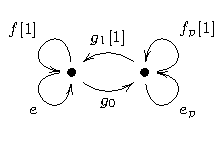
\includegraphics[width=0.26\linewidth]{figures/quiver.pdf}
\end{center}

本节余下部分概述如何建立下述结果：

\begin{proposition}\label{prop:6.2}
在上述记号下，有
\[
HH^{d,2-d}(Q)=\begin{cases}k, & d=6,8,\\ 0, & d>2,\ d\neq6,8.\end{cases}
\]
\end{proposition}

在此之前，我们先说明下述重要推论，它是整个计算的动机。该推论把我们的 Hochschild 上同调计算的含义明确写出，所用工具是定理 \ref{thm:5.3} 关于 Hochschild 上同调与 $A_\infty$-结构关系的理论，连同定理 \ref{thm:2.1} 的同调微扰论。

\begin{corollary*}
每个满足 $H(\mathcal{Q}')\simeq Q$ 的 $A_\infty$-代数 $(\mathcal{Q}',m_d)$ 都拟同构于一个极小 $A_\infty$-代数 $(\tilde{\mathcal{Q}},\tilde m_d)$，使得 $\tilde m_d=0$ 对 $d\le5$ 或 $d=7$。结构映射 $\tilde m_6$ 与 $\tilde m_8$ 在 $HH^{6,-4}(A)$ 与 $HH^{8,-6}(A)$ 中定义上链。

此外，若 $(\mathcal{Q}',m_d)$ 与 $(\mathcal{Q}'',m'_d)$ 是如上两个极小 $A_\infty$-代数，且 $[m_6]=[m'_6]$、$[m_8]=[m'_8]$，则 $\mathcal{Q}'$ 与 $\mathcal{Q}''$ 规范等价。

特别地，$Q$ 上 $A_\infty$-结构在拟同构意义下的空间至多是一维的。
\end{corollary*}

% [Tutor Note: 原文疑误：推论中写 $HH^{6,-4}(A)$ 与 $HH^{8,-6}(A)$，但本推论讨论的是 $Q$ 上的 $A_\infty$-结构，应为 $HH^{6,-4}(Q)$ 与 $HH^{8,-6}(Q)$（与 p.25 及命题 6.2 的写法一致）。译文保留原文写法。]

% [Tutor Note: 推论中“极小”指 $m_1=0$；homological perturbation 保证任何 $A_\infty$-代数都拟同构于极小的一个。注意 $m_6$ 与 $m_8$ 分别对应 $HH^{6,-4}$ 与 $HH^{8,-6}$：$m_d$ 的次数为 $2-d$，故落在第二个指标 $2-d$ 上，这不是笔误。]

证明的出发点是观察 $HH^{m,n}(A)=\Ext^m_{A\otimes A^{op}}(A,A(n))$（见第 \ref{subsec:hoch-cohomology} 小节）。因此，可以通过为有限维分次代数 $Q^e=Q\otimes Q^{op}$ 找到一个显式的投射消解来建立该定理。这看起来相当没有启发性。所以我们先看看用更抽象的论证能得到什么。

现在的关键观察是：$Q$ 是域上的有限维代数。这开启了一大套一般理论，参见例如 [22]。（该文献处理的是未分次的代数与模，但到分次情形的改造是直接的。）

$Q$ 的极小幂等元是 $e_1=e$ 与 $e_2=e_p$。由此可知 $P_i=Qe_i$（$i=1,2$）是极小不可分解投射 $Q$-模，且所有这些模都具有 $P_i(n)$ 的形式（对某个 $n$）。这些投射模有唯一的非平凡单商模 $S_i$，而这样我们就再次得到全部单 $Q$-模。事实上，$S_i$ 是一维 $k$-向量空间，分别由 $e$ 与 $e_p$ 的类张成。

由一般理论可知，$Q^e$ 的极小投射模是 $P_{ij}(m)=(e_iQe_j)(m)$，单模是 $S_{ij}(m)=\Hom_k(S_i,S_j)(m)$。于是，把 [7] 中引理 1.5 的论证改造到分次情形，我们得到：

\begin{lemma*}
设 $\cdots\to R_n\to R_{n-1}\to\cdots\to R_1\to R_0\to Q$ 是 $Q$ 作为 $Q^e$-模的极小投射消解。则
\[
R_n=\bigoplus_{i,j,m}P_{i,j}(m)^{\Ext^n_Q(S_i,S_j(m))}.
\]
\end{lemma*}

现在容易验证存在正合列
\begin{gather*}
0\longleftarrow S_1\longleftarrow P_1\xleftarrow{\ \times g_0\ }P_1\xleftarrow{\ \times f_p\ }S_2(-1)\longleftarrow 0\\
0\longleftarrow S_2\longleftarrow P_2\xleftarrow{\ \times g_1\ }P_2(-1)\xleftarrow{\ \times f\ }S_1(-2)\longleftarrow 0
\end{gather*}
从而存在如下投射消解：
\begin{gather*}
\cdots\to P_1(-3)\to P_1(-3)\xrightarrow{\ \cdot\ }P_2(-2)\to P_2(-1)\to P_1\to P_1\to S_1\to 0\\
\cdots\to P_2(-4)\to P_2(-3)\xrightarrow{\ \cdot\ }P_1(-2)\to P_1(-2)\to P_2(-1)\to P_2\to S_2\to 0
\end{gather*}
忽略分次后，这些消解以四为周期。带点的箭头表示第一个周期的结束；当然，末尾的 $S_i\to0$ 部分不重复。经过每个周期后，分次增加三。

% [Tutor Note: 核对要点：两个短正合列并不对称——第一列是 $S_1\leftarrow P_1\leftarrow P_1\leftarrow S_2(-1)$（第二个 $P_1$ 无平移），第二列是 $S_2\leftarrow P_2\leftarrow P_2(-1)\leftarrow S_1(-2)$。“无平移”与“$(-1)$”的差别正是把 $S_2(-1)$、$S_1(-2)$ 逐步代换、拼出周期消解的关键；抄写时不要“顺手补齐对称性”。]

% [Tutor Note: 消解中的映射都是左乘相应元素（$\times g_0$、$\times f_p$ 等）。带点箭头的“周期”是：$S_1$ 的消解由 $S_2(-1)$ 的消解接续，而 $S_2(-1)$ 的消解又由 $S_1(-3)$ 的消解接续，如此循环，每循环一次整体平移 $-3$，故“分次增加三”。]

现在注意到 $\Hom_Q(P_i(n),S_j(m))=\Hom_Q(S_i(n),S_j(m))$ 在 $i=j=n=m$ 之外为零，于是由引理推出：类似地，$Q$ 在 $Q^e$ 上有一个投射消解，忽略分次时以八为周期，且经过每个周期后分次增加六。

特别地，由此可知对任意 $l$，当 $n$ 充分大时 $HH^{n,l-n}(Q)=0$。事实上，它是 $\Hom_{Q^e}(R_n,Q(l-n))=\Hom_{Q^e}(R_n([6n/8]),Q(l-n+[6n/8]))$ 的一个子商，而由消解的周期性，$R_n([6n/8])$ 只依赖于 $n\pmod 8$，同时 $Q(l-n+[6n/8])$ 终将落在任意高的次数上。这里 $[x]$ 表示不超过 $x$ 的最大整数。

% [Tutor Note: 注意第二个指标：前一句用一般参数 $l$（即 $HH^{n,l-n}$），后一句取 $l=2$（即 $HH^{n,2-n}$），因为 $A_\infty$-结构的形变方向是 $HH^{\bullet,2-\bullet}$（$m_d$ 的次数为 $2-d$）。这是本页最易混的下标，命题 6.2 与推论的指标都由它决定。]

更仔细一些，容易确切找出极小投射消解中出现的模，并给出使 $HH^{n,2-n}=0$ 成立的 $n$ 的显式下界。于是证明该命题就只剩两件事：把 $Q$ 的投射消解具体算到有限长度（例如真正确定消解中模之间的映射），并计算低维 Hochschild 上同调。这是件苦差事，最好交给计算机。若有特别受虐狂的读者想手工验证，她会受益于这样一个事实：不仅极小投射消解中的模是周期的，映射也是周期的。因此整个命题可以通过找出这个周期消解来建立。详细计算已在 [12, 定理 4] 中完成。

该命题也在 [11] 中用（不同的）方法重新证明过。

% [Tutor Note: 作者省略的全部计算是：$Q$ 的极小投射消解周期为 8、映射亦周期（正文明说），因此只需把前 8 步的映射矩阵写出、并对 $n=0,\dots,7$ 计算 $\Ext^n$；$HH^{d,2-d}=k$ 只在 $d=6,8$ 出现，正好解释了为什么只有 $m_6,m_8$ 无法被平凡化。可用矩阵模型 $Q\subset M_2(k[s]/s^2)$ 手算，或按 [12] 的程序实现。]
    % §5 Hochschild cohomology / §6 (up to 6.1)
% ============================================================
%  sec06b.tex —— §6.2 椭圆曲线的导出范畴 / §6.3 环面的 Fukaya 范畴
%  对应原文 pp.29–38（含无编号小节 Equivariant $A_\infty$-structures and
%  Weierstrass cubics、Generation、Counting polygons）
%  本文件不含 \section：§6 的 \section 与 §6.1 在 sec05_06a.tex 中。
% ============================================================

\subsection{椭圆曲线的导出范畴}\label{subsec:6.2}

固定一个特征零的代数闭域 $k$。令 $E$ 为光滑射影曲线，$P\in E$ 为闭点。由关于曲线导出范畴生成元的定理~\ref{thm:3.3}，$\mathcal{L}=\mathcal{O}_E\oplus\mathcal{O}_E(P)$ 是分裂生成元（split-generator）。由第~\ref{sec:derived} 节中 $D_\infty(E)$ 的构造、特别是命题~\ref{prop:3.1}，有
\[
\mathrm{Hom}_{HD_\infty(E)}(\mathcal{L},\mathcal{L})=\mathrm{Ext}^*(\mathcal{L},\mathcal{L}).
\]
这个分次代数的向量空间结构可以完全形式地确定；我们先做这一步。

% [Tutor Note: 易错点：Serre 对偶 $H^k(X,\mathcal{L})\cong H^{n-k}(X,\mathcal{L}^{\vee}\otimes\omega_X)^{\vee}$ 右端的对偶取自整个向量空间，而非层的对偶。对椭圆曲线 $n=1$、$\omega_X\cong\mathcal{O}_X$ 平凡，故 $H^1(E,\mathcal{L})\cong H^0(E,\mathcal{L}^{\vee})^{\vee}$；这是本节所有 Ext 群计算（尤其 $h_0h_1\neq0$、$h_1h_0\neq0$）的唯一非形式输入。]

事实上，回忆概形上 Ext 群的一些基本性质（见文献 [8] 第 III.6 节）：(1) 若 $\mathcal{L}$ 局部自由而 $\mathcal{F},\mathcal{G}$ 凝聚，则 $\mathrm{Ext}^*(\mathcal{L}\otimes\mathcal{F},\mathcal{G})=\mathrm{Ext}^*(\mathcal{F},\mathcal{L}^{\vee}\otimes\mathcal{G})$；(2) $\mathrm{Ext}^*(\mathcal{O}_X,\mathcal{F})=H^*(X,\mathcal{F})$；(3) $\mathrm{Ext}^*$ 是双线性的。这里 $\mathcal{L}^{\vee}$ 表示对偶层。这三条都是关于 $\mathrm{Hom}=\mathrm{Ext}^0$ 的相应陈述与导出函子泛性的容易推论。再回忆 Serre 对偶（见文献 [8] 第 III.7 节）：若 $X$ 是 $n$ 维光滑射影概形，则
\[
H^k(X,\mathcal{L})\cong H^{n-k}(X,\mathcal{L}^{\vee}\otimes\omega_X)^{\vee}.
\]

现在回到 $X=E$、$\mathcal{L}=\mathcal{O}_E\oplus\mathcal{O}_E(P)$ 的情形。此后我们一并省略下标 $E$。利用双线性，可以把 Ext 代数分解为“矩阵元”：
\begin{equation}\label{eq:6.2-1}
\mathrm{Ext}^*(\mathcal{L},\mathcal{L})=
\begin{pmatrix}
\mathrm{Ext}^*(\mathcal{O},\mathcal{O}) & \mathrm{Ext}^*(\mathcal{O}(P),\mathcal{O})\\[2pt]
\mathrm{Ext}^*(\mathcal{O},\mathcal{O}(P)) & \mathrm{Ext}^*(\mathcal{O}(P),\mathcal{O}(P))
\end{pmatrix}.
\end{equation}
这句话的意思是：左端作为向量空间分解为右端四个子空间的直和，而左端的乘法对应右端的矩阵乘法，再复合上 $\mathrm{Ext}^*=\mathrm{Hom}_{HD_\infty(E)}$ 上的外乘法。此外，我们可以用性质 (1)、(2) 连同 Serre 对偶，把上式用层上同调空间表出。

% [Tutor Note: 易错点：这里的“矩阵乘法”指由两个直和因子诱导的分块乘法，交叉项 $h_0h_1$、$h_1h_0$ 的符号遵循 Koszul 约定（$h_1$ 是度为 1 的奇元素）；原文只关心非零性，故未写符号。又，原文此句把 $\mathrm{Ext}^*=\mathrm{Hom}_{HD_\infty(E)}$ 的变量省略了，应读作 $\mathrm{Ext}^*(\mathcal{L},\mathcal{L})=\mathrm{Hom}_{HD_\infty(E)}(\mathcal{L},\mathcal{L})$；译文保留原文省略写法。]

下面特殊化到椭圆曲线情形，得到：

\begin{proposition}\label{prop:6.3}
设 $E$ 是特征零代数闭域 $k$ 上的椭圆曲线，$P\in E$ 为闭点。则
\[
\mathrm{Ext}^*(\mathcal{O}\oplus\mathcal{O}(P),\mathcal{O}\oplus\mathcal{O}(P))\xrightarrow{\ \sim\ }Q,
\]
其中 $Q$ 是上一小节的分次代数。
\end{proposition}

\begin{proof}
绝大部分工作已经完成。我们有 $H^0(E,\mathcal{O})=k$（即 $E$ 上没有非常值正则函数，这对任何连通射影概形都成立），于是特别地 $H^0(E,\mathcal{O}(-P))=0$（因为 $\mathcal{O}(-P)$ 是在 $P$ 处取零的正则函数构成的层）。又 $H^0(E,\mathcal{O}(P))=k$，因为 $E$ 不可能具有只有一个单极点的有理函数（否则它就同构于 $\mathbb{P}^1$）。注意到椭圆曲线的典范丛平凡，这些计算已足以说明我们的 Ext 代数作为分次向量空间同构于 $Q$。

但 $A$ 中本质上所有合成都已由形式理由确定（即由 $\mathcal{O}$ 与 $\mathcal{O}(P)$ 的单位元的作用，以及次数理由）。令 $h_0$ 表示 $\mathrm{Hom}(\mathcal{O},\mathcal{O}(P))$ 中的非零元，$h_1$ 表示 $\mathrm{Ext}^1(\mathcal{O}(P),\mathcal{O})$ 中的非零元。为完成证明，只需说明 $h_0h_1\neq0$ 且 $h_1h_0\neq0$，因为这是仅剩的尚未确定的合成。

% [Tutor Note: 原文此处记号 $A$ 未加定义，从上下文看它就是本段所论的 Ext 代数 $\mathrm{Ext}^*(\mathcal{L},\mathcal{L})$（原文此处作斜体 $A$、而非花体 $\mathcal{A}$；按行文它也可能是想写 §6.1 的 $Q$，但 $Q$ 此时只被证明为分次向量空间同构，尚不能直接当作代数使用）。译文保留原文记号。]

我们有正合列 $0\to\mathcal{O}\to\mathcal{O}(P)\to\mathcal{O}/P\to0$，其中第一个映射是 $h_0$。作用 $\mathrm{Ext}^*(\mathcal{O}(P),\bullet)$ 得到
\[
\mathrm{Ext}^1(\mathcal{O}(P),\mathcal{O})\xrightarrow{\ \times h_0\ }\mathrm{Ext}^1(\mathcal{O}(P),\mathcal{O}(P))\to\mathrm{Ext}^1(\mathcal{O}(P),\mathcal{O}/P).
\]
但 $\mathrm{Ext}^1(\mathcal{O}(P),\mathcal{O}/P)=H^1(E,\mathcal{O}/P)$（因为 $\mathcal{O}/P$ 是摩天楼层），而该群为零（摩天楼层是松弛的，即 flasque）。因此右乘 $h_0$ 是满射，且 $h_1h_0\neq0$。

% [Tutor Note: 作者省略的两步：($i$) $\mathrm{Ext}^1(\mathcal{O}(P),\mathcal{O}/P)=H^1(E,\mathcal{O}/P)=0$ 的理由是 $\mathcal{O}/P$ 为摩天楼层，而松弛层无高次上同调；($ii$) 后文 $\mathrm{Ext}^2(\mathcal{O}/P,\mathcal{O})=0$ 由对 $0\to\mathcal{O}\to\mathcal{O}(P)\to\mathcal{O}/P\to0$ 作用 $\mathrm{Ext}^*(\mathcal{O},\bullet)$ 并利用 $H^2(X,\mathcal{F})=0$ 得到，而后者对线丛成立——对椭圆曲线这正是 Serre 对偶 $H^2\cong H^0(\mathcal{F}^{\vee})^{\vee}=0$。]

改作用 $\mathrm{Ext}^*(\bullet,\mathcal{O})$，则得到
\[
\mathrm{Ext}^1(\mathcal{O}(P),\mathcal{O})\xrightarrow{\ h_0\times\ }\mathrm{Ext}^1(\mathcal{O},\mathcal{O})\to\mathrm{Ext}^2(\mathcal{O}/P,\mathcal{O}).
\]
只要确立 $\mathrm{Ext}^2(\mathcal{O}/P,\mathcal{O})=0$，前面的论证就同样行得通。而这可由对我们的正合列作用 $\mathrm{Ext}^*(\mathcal{O},\bullet)$、并注意到对任意线丛 $\mathcal{F}$ 有 $H^2(X,\mathcal{F})=0$（由 Serre 对偶）得到。
\end{proof}

我们指出：若 $P$ 是光滑点，则上述结果对奇异三次曲线仍然成立，只是此时论证要稍微仔细一些。

\subsubsection{\texorpdfstring{等变 $A_\infty$-结构与 Weierstrass 三次曲线}{等变 A∞-结构与 Weierstrass 三次曲线}}\label{subsec:equivariant-ainf}

我们希望论证：由椭圆曲线得到的 $Q$ 上的 $A_\infty$-结构本质上穷尽了所有可能（有两个例外，一个形式、一个非形式）。

具体地说，固定一条三次曲线 $E$ 与一个光滑点 $P$，并置
\[
\mathcal{Q}_{E,P}=\mathrm{Hom}_{D_\infty(E)}(\mathcal{O}_E\oplus\mathcal{O}_E(P),\mathcal{O}_E\oplus\mathcal{O}_E(P)).
\]
这是一个 DGA（微分分次代数），在拟同构意义下良定义；由前面的命题~\ref{prop:6.3}，有 $H(\mathcal{Q}_{E,P})\xrightarrow{\sim}Q$。于是由同调微扰论，我们得到 $Q$ 上的极小 $A_\infty$-结构 $(m_d^{E,P})$。

我们希望说：这样一来就得到了所有同构类的 $A_\infty$-结构。这件事出人意料地棘手。我们沿用文献 [11] 的方法，即研究如何把所有的 $\mathcal{Q}_{E,P}$ 一致地变成极小 $A_\infty$-代数。

% [Tutor Note: 几何直观：$\mathcal{Q}_{E,P}$ 是“把曲线上的两个对象 $\mathcal{O}$ 与 $\mathcal{O}(P)$ 之间的全部 Ext 群堆成一个 dg 代数”；它依赖 $E,P$ 的选取，但只在拟同构意义下良定义。同调微扰论把它的极小模型搬到 $H(\mathcal{Q}_{E,P})\cong Q$ 上，于是“椭圆曲线的 $A_\infty$-结构”就变成 $Q$ 上的一族极小 $A_\infty$-结构——这正是接下来用 Weierstrass 族统一处理它们的动机。]

更确切地说，置 $R=k[a,b]$，并令 $W=R(k)$。然后考虑曲线族
\[
\mathcal{X}=\{X_0Y^2=X^3+aX_0^2X+bX_0^3\}\subset\mathbb{P}^2_R,
\]
连同它到 $\mathrm{Spec}(R)=\mathbb{A}^2$ 的自然映射。乘法群 $\mathbb{G}_m$（其中 $\mathbb{G}_m(k)=k^{\times}$）通过
\[
a^u=u^4a,\qquad b^u=u^6b\qquad (u\in k^{\times})
\]
作用在 $R$ 上；它作用在 $\mathcal{X}$ 上为
\[
((X_0:X:Y),(a,b))^u=((X_0:u^2X:u^3Y),(u^4a,u^6b)),
\]
覆盖了它在 $\mathrm{Spec}(R)$ 上的作用。对 $w=(w_1,w_2)\in W$，记 $k(w)=R/(a-w_1,b-w_2)$ 为剩余域，$\mathcal{X}_w=\mathcal{X}\times_R k(w)$ 为纤维。$\mathbb{G}_m$ 在 $\mathcal{X}$ 上的作用诱导同构 $u:\mathcal{X}_w\to\mathcal{X}_{w^u}$。

% [Tutor Note: 易错点（权与分次的对应）：$\mathbb{G}_m$ 对 $a,b$ 的权为 $(u^4,u^6)$，对坐标为 $X_0\mapsto u^0X_0$、$X\mapsto u^2X$、$Y\mapsto u^3Y$；这组权恰好使三次方程 $X_0Y^2=X^3+aX_0^2X+bX_0^3$ 的每一项权都为 $6$。$A_\infty$ 结构映射 $m_d$ 的度为 $2-d$，正是这个 $2-d$ 导致等变关系 $m_d^{w^u}=u^{d-2}m_d^w$（见后文引理第 1 条），也使 $m_6,m_8$ 的权分别等于 $-4,-6$，从而与 $a,b$ 的权 $4,6$ 通过 $d-2$ 对应：$6-2=4$，$8-2=6$。]

我们将构造一个 $R$ 上的、带 $k^{\times}$ 作用的 DGA $\mathcal{B}$。它将具有如下性质：$\mathcal{B}_w:=\mathcal{B}\otimes_R k(w)$ 拟同构于 $\mathcal{Q}_{\mathcal{X}_w,P_w}$；并且 $H(\mathcal{B})\otimes k(w)\to H(\mathcal{B}_w)$ 是同构。

所谓 $\mathcal{B}$ 的一个\textbf{等变分裂}（equivariant splitting），是指一个分解
\[
\mathcal{B}=H\oplus\mathrm{im}(d)\oplus T,
\]
其中所有直和项都是 $k^{\times}$-不变的，且 $H\oplus\mathrm{im}(d)=\ker(d)$。由此得到 $\mathcal{B}$ 的度为 $-1$ 的等变收缩 $r:\mathcal{B}\to\mathcal{B}$（$d:T\to\mathrm{im}(d)$ 是同构；令 $r|_{\mathrm{im}(d)}=d^{-1}$，在补空间上令 $r=0$）。若记 $i:H(\mathcal{B})\to\mathcal{B}$ 与 $p:\mathcal{B}\to H(\mathcal{B})=H$ 为自然映射，则 $r$ 是 $ip$ 与 $\mathbf{1}$ 之间的同伦。于是我们可以对 $H(\mathcal{B})$ 应用同调微扰引理~\ref{thm:2.1}，构造出一个 $R$ 上的极小 $A_\infty$-结构，记作 $\mathcal{A}$。由于 $H=H(\mathcal{B})$ 是 $k^{\times}$-等变的，$k^{\times}$ 作用在 $\mathcal{A}$ 上。我们将验证：它在度为 $i$ 的元素上的作用（$i=0$ 或 $i=1$ 是仅有的两种可能）是纯权 $i$ 的，即 $h^u=u^{|h|}h$，对 $h\in H$。对每个 $w\in W$，我们得到 $Q$ 上的极小 $A_\infty$-结构 $\mathcal{A}_w=\mathcal{A}\otimes_R k(w)$；记其结构映射为 $m_d^w$，它们是 $w$ 的各分量的（向量值）多项式。

% [Tutor Note: 这一步是整节的技术核心：先在 $k^{\times}$-等变分解 $\mathcal{B}=H\oplus\mathrm{im}(d)\oplus T$ 上做 Hodge 型“调和代表”选取，同调微扰论才具有等变性；否则微扰论给出的 $A_\infty$-结构会依赖 $R$ 上基的选取。“$H(\mathcal{B})$ 的 $k^{\times}$-作用纯权等于分次”这一条，是后文能把 $m_6,m_8$ 与 $a,b$ 直接对上的关键。]

带 $G$-作用的域上分次向量空间 $V$ 上的\textbf{等变 $A_\infty$-结构} $(m_d)$，指的是满足
\[
m_d(a_d^g,\ldots,a_1^g)=m_d(a_d,\ldots,a_1)^g\qquad(\forall d>0,\ a_i\in V,\ g\in G)
\]
的 $A_\infty$-结构。我们将验证 $\mathcal{B}$ 是一个 $k^{\times}$-等变 DGA。于是 $\mathcal{A}$ 上 $A_\infty$-结构的显式公式蕴含 $\mathcal{A}$ 是 $k^{\times}$-等变 $A_\infty$-代数。这一点连同我们对 $\mathcal{A}$ 上 $k^{\times}$-作用的计算，将推出
\[
m_d^{w^u}=u^{d-2}m_d^w.
\]
由于 $m_d^w$ 还是多项式，一个容易的计算将说明：当 $d<6$ 或 $d=7$ 时 $m_d^w=0$；$m_6^{(a,b)}=a$；$m_8^{(a,b)}=b$。由此可知 $A_\infty$-结构 $\mathcal{A}_w$ 自动满足 $m_i=0$（$i=3,4,5,7$），并且由命题~\ref{prop:6.2} 的推论（它计算了 $Q$ 的 Hochschild 上同调）穷尽了所有可能。

在核验上述论证的细节之前，我们先记录由它得到的下述定理：

\begin{theorem}\label{thm:6.4}
设 $\mathcal{C}$ 是分裂闭的三角 $A_\infty$-范畴，由对象 $\mathcal{O}$ 与 $\mathcal{O}(P)$ 生成。再设
\[
\mathrm{Hom}_{H^*(\mathcal{C})}(\mathcal{O}\oplus\mathcal{O}(P),\mathcal{O}\oplus\mathcal{O}(P))\simeq Q,
\]
其中 $Q$ 是命题~\ref{prop:6.2} 中的分次代数。
令 $\mathcal{O}/P$ 表示 $g_0:\mathcal{O}\to\mathcal{O}(P)$ 的锥，令 $S$ 表示分次环 $\bigoplus_n\mathrm{Hom}_{H^0(\mathcal{C})}\bigl(\mathcal{O},T_{\mathcal{O}/P}^{3n}(\mathcal{O})\bigr)$，并置 $E=\mathrm{Proj}(S)$。则 $E$ 可以嵌入 $\mathbb{P}^2$ 成为一条三次曲线（即 $S$ 由三个一次元素生成，它们满足一个齐次三次关系）；并且若 $E$ 光滑，则 $\mathcal{C}$ 与 $E$ 的增强导出范畴 $D_\infty(E)$ 之间存在 $A_\infty$-范畴的拟等价。
\end{theorem}

% [Tutor Note: 定理陈述中的 $\mathcal{O},\mathcal{O}(P),\mathcal{O}/P$ 是抽象三角范畴 $\mathcal{C}$ 里的对象记号，不是层；$\mathcal{O}/P$ 是 $g_0:\mathcal{O}\to\mathcal{O}(P)$ 的锥，$g_0$ 是 §6.1 中六维代数 $Q$ 的生成元。定理把“几何对象 $\mathcal{O}\oplus\mathcal{O}(P)$”抽象为“生成元及其关系代数为 $Q$”，这是后文重建定理的全部内容。]

\begin{proof}
令 $\mathcal{Q}'$ 表示由 $\mathcal{C}$ 得到的 $Q$ 上的 $A_\infty$-代数结构。由上面的分类，$\mathcal{Q}'\simeq\mathcal{A}_w$ 对某个 $w$ 成立。若 $\mathcal{X}_w$ 光滑，其增强导出范畴 $D(\mathcal{X}_w)$ 由 $\mathcal{O}\oplus\mathcal{O}(P)$ 分裂生成，于是由关于分裂三角包络唯一性的定理~\ref{thm:2.4}，$\mathcal{C}$ 拟等价于 $D(\mathcal{X}_w)$。即使 $\mathcal{X}_w$ 不光滑，$\mathcal{C}$ 也拟等价于 $\mathcal{O}\oplus\mathcal{O}(P)$ 的分裂闭三角包络，即 $D(\mathcal{X}_w)$ 的一个子范畴（包含所有 $\mathcal{O}(nP)$）。此外，$\mathcal{C}$ 中算出的环同构于 $D_\infty(\mathcal{X}_w)$ 中算出的环，这一点由关于用扭变函子定义的全自同态环的命题~\ref{prop:2.6} 给出。

现在注意 $\mathrm{Ext}^*(\mathcal{O}/P,\mathcal{O}(nP))$ 是一维的，且生成元在度 $1$。因此 $T_{n+1}:=T_{\mathcal{O}/P}(\mathcal{O}(nP))$ 落在特殊三角形
\[
\mathcal{O}/P[-1]\to\mathcal{O}(nP)\to T_{n+1}\to
\]
中。我们有正合列 $0\to\mathcal{O}(nP)\to\mathcal{O}((n+1)P)\to\mathcal{O}/P\to0$，它给出特殊三角形
\[
\mathcal{O}/P[-1]\to\mathcal{O}(nP)\to\mathcal{O}((n+1)P)\to.
\]
于是 $T_{n+1}\simeq\mathcal{O}((n+1)P)$，因为两者都是某个非零态射的锥，而这样的态射在相差一个非零倍数的意义下唯一。因此 $T_{\mathcal{O}/P}^{3n}(\mathcal{O})=\mathcal{O}(3nP)$。

于是只剩下证明下述事实：固定 $w\in W$，令 $S=\bigoplus_n\mathrm{Hom}_{D^b(\mathrm{Coh}(\mathcal{X}_w))}(\mathcal{O},\mathcal{O}(3nP))$，则 $\mathrm{Proj}(S)$ 同构于 $\mathcal{X}_w$。但这是显然的（因为 $\mathcal{O}(3P)$ 极丰富）。
\end{proof}

% [Tutor Note: 定理证明末尾“显然”一句的实质：$\mathcal{O}(3P)$ 极丰富，故它给出 $\mathcal{X}_w\hookrightarrow\mathbb{P}^2$ 的三次嵌入，于是 $\mathrm{Proj}\bigl(\bigoplus_nH^0(\mathcal{O}(3nP))\bigr)\cong\mathcal{X}_w$；这一步是整个证明中唯一把范畴里的环 $S$ 反推回曲线 $E$ 的“重建”输入，也是定理~\ref{thm:6.4} 能成为重建定理的原因。]

$\mathcal{X}$ 被两个仿射开集 $U=\{X_0\neq0\}$ 与 $V=\{X_2\neq0\}$ 覆盖。对这个覆盖记 $\mathcal{U}=\{U,V\}$。

$\mathcal{X}$ 有光滑子簇 $P=\{X_0=0\}$。我们置
\[
\mathcal{B}=\check{C}^\bullet\bigl(\mathcal{U},\mathcal{H}om(\mathcal{O}_{\mathcal{X}}\oplus\mathcal{O}_{\mathcal{X}}(P),\mathcal{O}_{\mathcal{X}}\oplus\mathcal{O}_{\mathcal{X}}(P))\bigr).
\]
这里 $\check{C}^\bullet(\mathcal{U},\mathcal{F})$ 表示关于覆盖 $\mathcal{U}$、系数在层 $\mathcal{F}$ 中的 Čech 复形。

\begin{lemma*}\label{lem:b-dga}
$\mathcal{B}$ 具有所要求的性质。即：
\begin{enumerate}
  \item\label{lem:B-1} $\mathcal{B}$ 是 DGA，
  \item\label{lem:B-2} $k^{\times}$ 作用在 $\mathcal{B}$ 上，
  \item\label{lem:B-3} $\mathcal{B}$ 的微分与乘法是 $k^{\times}$-等变的，
  \item\label{lem:B-4} $\mathcal{B}$ 容许一个 $k^{\times}$-等变分裂，
  \item\label{lem:B-5} $H(\mathcal{B})\otimes k(w)\to H(\mathcal{B}_w)$ 是同构，且 $\mathcal{B}_w$ 拟同构于 $\mathcal{Q}_{\mathcal{X}_w,P_w}$，
  \item\label{lem:B-6} $k^{\times}$ 在 $H(\mathcal{B}_w)$ 上作用的权与分次一致。
\end{enumerate}
\end{lemma*}

\begin{proof}
置 $\mathcal{F}=\mathcal{H}om(\mathcal{O}_{\mathcal{X}}\oplus\mathcal{O}_{\mathcal{X}}(P),\mathcal{O}_{\mathcal{X}}\oplus\mathcal{O}_{\mathcal{X}}(P))$。回忆 $\mathcal{O}_{\mathcal{X}}(P)$ 是“沿光滑余维一子簇 $P$ 至多一阶极点”的函数所成的线丛。确切地说，作为函数域 $K(\mathcal{X})$ 的子集，
\[
\mathcal{O}_{\mathcal{X}}(P)(U)=\mathcal{O}_{\mathcal{X}}(U),\qquad
\mathcal{O}_{\mathcal{X}}(P)(V)=\frac{x}{y}\mathcal{O}_{\mathcal{X}}(V).
\]

(1) $\mathcal{B}$ 上有自然乘法，它来自杯积 $\check{C}^p(\mathcal{U},\mathcal{F})\times\check{C}^q(\mathcal{U},\mathcal{F})\to\check{C}^{p+q}(\mathcal{U},\mathcal{F})$ 与同态复合映射 $\mathcal{F}\otimes\mathcal{F}\to\mathcal{F}$。

(2) $\mathbb{G}_m$ 作用在 $\mathcal{X}$ 上，从而 $k^{\times}$ 作用在 $K(\mathcal{X})$ 上。由于 $\mathbb{G}_m$-作用保持 $U,V$ 与 $P$，故 $k^{\times}$ 作用在 $\mathcal{B}$ 上。

(3) 有典范同构 $\mathcal{F}=\mathcal{O}\oplus\mathcal{O}(P)\oplus\mathcal{O}(-P)\oplus\mathcal{O}$（“矩阵元”）。于是乘法映射 $\mathcal{F}\times\mathcal{F}\to\mathcal{F}$ 对应 $K(\mathcal{X})$ 中元素的实际乘法。杯积显然是 $k^{\times}$-等变的，故 $\mathcal{B}$ 上的乘法也是。微分就是 Čech 微分，它同样显然是等变的。

(4) 只需分别考察矩阵元 $\mathcal{O}_{\mathcal{X}}$ 与 $\mathcal{O}_{\mathcal{X}}(\pm P)$。先看 $\mathcal{O}_{\mathcal{X}}$。注意 $\mathcal{O}_{\mathcal{X}}(U)$ 是以 $x^iy^j$（$i\ge0,\ j=0,1$）为基的自由 $R$-模；类似地，$\mathcal{O}_{\mathcal{X}}(V)$ 是以 $u^iv^j$ 为基的自由 $R$-模，其中 $u=1/y$、$v=x/y$，且 $i\ge0$、$v=0,1,2$。$\check{C}^0(\mathcal{U},\mathcal{O}_{\mathcal{X}})\to\check{C}^1(\mathcal{U},\mathcal{O}_{\mathcal{X}})$ 的核由以 $(1,1)$ 为基的自由 $R$-模给出，它显然是等变的，并且容许一个等变补空间。$\mathcal{O}_{\mathcal{X}}(U\cap V)$ 是以 $x^iy^j$（$i\in\mathbb{Z}$，$j\le1$）为基的自由 $R$-模。$\check{C}^0(\mathcal{U},\mathcal{O}_{\mathcal{X}})\to\check{C}^1(\mathcal{U},\mathcal{O}_{\mathcal{X}})$ 的像是以 $x^iy^j$（$(i,j)\neq(1,-2)$）为基的自由 $R$-模。这同样是等变的，并有显然的等变补空间。$\mathcal{O}_{\mathcal{X}}(\pm P)$ 的情形可用类似的论证处理。

% [Tutor Note: 原文疑误：第 (4) 条中“$\mathcal{O}_{\mathcal{X}}(V)$ 以 $u^iv^j$ 为基，$u=1/y$、$v=x/y$，且 $i\ge0$、$v=0,1,2$”的最后一个 $v$ 应为 $j$（即 $j=0,1,2$），否则与单项式 $u^iv^j$ 中的 $v$ 冲突。译文保留原文写法并在此标注。]

(5) $\mathcal{B}_w$ 自然同构于
\[
\check{C}^\bullet\bigl(\{U_w,V_w\},\mathcal{H}om(\mathcal{O}_{\mathcal{X}_w}\oplus\mathcal{O}_{\mathcal{X}_w}(P_w),\mathcal{O}_{\mathcal{X}_w}\oplus\mathcal{O}_{\mathcal{X}_w}(P_w))\bigr).
\]
为看出它拟同构于
\[
\mathcal{Q}_{\mathcal{X}_w,P_w}=\mathrm{Hom}_{D_\infty(\mathcal{X}_w)}(\mathcal{O}_{\mathcal{X}_w}\oplus\mathcal{O}_{\mathcal{X}_w}(P_w),\mathcal{O}_{\mathcal{X}_w}\oplus\mathcal{O}_{\mathcal{X}_w}(P_w)),
\]
只需注意：对任何带内射消解 $I^\bullet$ 的局部自由层 $\mathcal{L}$，有拟同构图
\[
\begin{array}{ccccc}
\check{C}^\bullet\mathcal{H}om(\mathcal{L},\mathcal{L}) & \xrightarrow{\ a\ } &
\mathrm{Tot}\,\check{C}^\bullet\mathcal{H}om^\bullet(\mathcal{L},I) & \xleftarrow{\ b\ } &
\mathrm{Tot}\,\check{C}^\bullet\mathcal{H}om^\bullet(I,I)\\[4pt]
& & & & \Big\uparrow\scriptstyle{c}\\[-6pt]
& & & & \mathrm{Hom}^\bullet(I,I).
\end{array}
\]
事实上，$\mathrm{Tot}\,\check{C}^\bullet$ 计算超上同调，而超上同调通过拟同构分解；$b$ 所对应的层复形之间的映射由命题~\ref{prop:3.1} 是拟同构（关于超上同调的基本事实见文献 [23] 第 5.7 节）。对任何内射层 $J$ 与凝聚层 $\mathcal{F}$，$\mathcal{H}om(\mathcal{F},J)$ 是松弛的、从而是无圈的，故 $\mathcal{H}om^\bullet(I,I)$ 的超上同调就是其整体截面的上同调；于是 $c$ 是拟同构。但我们已经知道
\[
\mathrm{Ext}^*(\mathcal{L},\mathcal{L})=H^*(\mathcal{L}^{\vee}\otimes\mathcal{L})
=H^*(\mathcal{H}om(\mathcal{L},\mathcal{L}))=\check{C}^*(\mathcal{H}om(\mathcal{L},\mathcal{L})),
\]
所以 $a$ 也是拟同构。

% [Tutor Note: 这里的“三段式拟同构”是标准论证：$\mathrm{Tot}\,\check{C}^\bullet$ 计算超上同调，而超上同调只依赖层的拟同构类，因此对两个变量分别取内射消解都给出同一个 $\mathrm{Ext}$ 群；$c$ 是拟同构用到了“内射层的 $\mathcal{H}om$ 是松弛层，从而无高次上同调”。注意本文约定 $\mathrm{Ext}^*(\mathcal{L},\mathcal{L})=H^*(\mathcal{L}^{\vee}\otimes\mathcal{L})$，这用到了 $\mathcal{L}$ 局部自由。]

于是 $H(\mathcal{B})\otimes k(w)\to H(\mathcal{B}_w)$ 是同构（两端我们都已算出！）。

(6) $H^0(\mathcal{X},\mathcal{O}_{\mathcal{X}})=k$ 带权为零的 $k^{\times}$-作用，$\mathcal{O}_{\mathcal{X}}(\pm P)$ 同理。$H^1(\mathcal{X},\mathcal{O}_{\mathcal{X}})$ 由 Čech 上链 $x^2/y$ 代表，它的权为一。$\mathcal{O}_{\mathcal{X}}(\pm P)$ 的情形同样可用类似的论证处理。
\end{proof}

回忆第~\ref{lem:B-5} 条，它使我们可以为 $\mathcal{B}$ 构造一个 $k^{\times}$-等变的极小模型 $\mathcal{A}$。下面我们利用第~\ref{lem:B-6} 条。

\begin{lemma*}\label{lem:weights}
\begin{enumerate}
  \item\label{lem:wt-1} 对 $u\in k^{\times}$，$m_d^{w^u}=u^{d-2}m_d^w$；
  \item\label{lem:wt-2} 当 $d=3,4,5$ 或 $d=7$ 时 $m_d^w=0$；
  \item\label{lem:wt-3} 把 $HH^{6,-4}(A)$ 与 $HH^{8,-6}(A)$ 与 $k$ 等同。则映射
  \[
  w\longmapsto\bigl([m_6^w],[m_8^w]\bigr)\in HH^{6,-4}(A)\oplus HH^{8,-6}(A)\simeq k^2
  \]
  由 $(a,b)\mapsto(Ca,Db)$ 给出，其中 $C$ 与 $D$ 是非零常数。
\end{enumerate}
\end{lemma*}

\begin{proof}
回忆 $m_d(a_d^u,\ldots,a_1^u)=m_d(a_d,\ldots,a_1)^u$。左端等于 $m_d^{(a,b)}([a_d]^u,\ldots,[a_1]^u)$，而右端等于 $m_d^{(a,b)^u}([a_d],\ldots,[a_1])^u$。利用第~\ref{lem:B-6} 条，这推出
\[
m_d^w([a_d],\ldots,[a_1])\,u^{|a_d|+\cdots+|a_1|}
=m_d^{w^u}([a_d],\ldots,[a_1])\,u^{|a_d|+\cdots+|a_1|+2-d}.
\]
（多出来的因子 $u^{2-d}$ 来自 $m_d$ 的度为 $2-d$。）这立刻推出第~\ref{lem:wt-1} 条。

现在我们知道 $m_d^w$ 是从 $W$ 到某个向量空间（即 $\mathrm{Hom}(Q^{\otimes d},Q(2-d))$）的函数，且在我们选定的基下具有多项式分量。令 $f(a,b)$ 为其中一个分量。我们知道
\[
f(u^4a,u^6b)=u^{d-2}f(a,b).
\]
对 $u$ 求导并令 $u=1$，得到
\begin{equation}\label{eq:6.2-2}
4a\frac{\partial f}{\partial a}+6b\frac{\partial f}{\partial b}=(d-2)f.
\end{equation}
这一步将分别作用于 $f$ 的每个齐次分量。设 $f$ 是 $r$ 次齐次的。则 $a\frac{\partial f}{\partial a}+b\frac{\partial f}{\partial b}=rf$，于是对某个常数 $\alpha$ 有 $b\frac{\partial f}{\partial b}=\alpha f$。这只有在 $f$ 是纯幂（即 $f=a^r$ 或 $f=b^r$）时才可能。但此时方程~\eqref{eq:6.2-2} 蕴含 $4r=d-2$（若 $f=x^r$）或 $6r=d-2$（若 $f=y^r$）。故得第~\ref{lem:wt-2} 条。

最后，第~\ref{lem:wt-3} 条中除了 $C$ 与 $D$ 可能为零之外都是清楚的。然而若其中之一为零，则由命题~\ref{prop:6.2} 的推论的论证，我们这样至多得到 $Q$ 上两个同构类的 $A_\infty$-结构。但由定理~\ref{thm:6.4} 的论证，不同构的 $\mathcal{X}_w$ 给出不同构的 $A_\infty$-结构（因为可以由 $\mathcal{A}_w$ 恢复 $\mathcal{X}_w$ 的同构类）。这与椭圆曲线有无穷多个同构类矛盾。
\end{proof}

% [Tutor Note: 易错点（权与分次的对应）：此处 $h^u=u^{|h|}h$ 是“纯权 $=|h|$”的定义，$m_d$ 的度为 $2-d$，故 $m_d^w$ 的权为 $d-2$ 而不是 $2-d$；微分方程 $4af_a+6bf_b=(d-2)f$ 必须与 Euler 齐次恒等式 $af_a+bf_b=rf$ 联立，而联立之前要先用“$f$ 的每个齐次分量各自满足该方程”把问题化到齐次情形，才能由 $bf_b=\alpha f$ 断言 $f$ 是纯幂，进而得到 $4r=d-2$ 或 $6r=d-2$。]

% [Tutor Note: 原文疑误：本页引理第 3 条中 $HH^{6,-4}(A)$、$HH^{8,-6}(A)$ 的 $A$ 在原文中排作斜体（而非花体 $\mathcal{A}$），按上下文应为极小模型 $\mathcal{A}$（第 30–31 页均记作 $\mathcal{A}$）。又，引理证明末句 “equation (4) implies that $4r=d-2$ (if $f=x^r$) or $6r=d-2$ (if $f=y^r$)” 中的 $x,y$ 应是 $a,b$（即 $f=a^r$ 或 $f=b^r$），否则与前面的 $f(a,b)$ 记号不符。译文均保留原记号并在此标注。]

\subsection{环面的 Fukaya 范畴}\label{subsec:6.3}

现在转向椭圆曲线同调镜像对称猜想的辛几何一侧。于是令 $T$ 表示标准环面 $\mathbb{R}^2/\mathbb{Z}^2$，带其标准辛结构与复结构。我们取对应于 $\Delta$ 的全纯平凡化的 Maslov 覆盖，于是所有非收缩的嵌入曲线以及所有辛同胚都可以分次（参见第~\ref{subsec:maslov} 小节的讨论）。以下始终用 $\mathrm{Fuk}$ 表示在上述选择下环面的 Fukaya 范畴。

\subsubsection{生成}\label{subsec:generation}

我们首先需要说明 $\mathrm{Fuk}$ 由两个对象生成，它们对应于 $\mathcal{O}$ 与 $\mathcal{O}/P$。取两条经线（meridian）$A$ 与 $B$（于是它们特别地自由生成 $H_1(T,\mathbb{Z})$）。为确定起见，我们假设基 $A,B$ 在其交点处为正向定向的；更具体地说，我们干脆假设 $A$ 对应直线 $(t,0)$，$B$ 对应直线 $(0,t)$。我们断言它们可作为生成元。我们打算使用关于用扭变判别分裂生成的定理~\ref{thm:2.7}：只需说明对 $X\in\mathrm{Fuk}$，存在 $n>0$ 使
\[
\mathrm{Hom}_{H^0(\mathrm{Fuk})}\bigl(X,(T_AT_B)^n(X)\bigr)=0.
\]
这显然是充分的。

\begin{definition*}\label{def:constant-sign}
设 $(M,\omega,\mathcal{L})$ 是分次流形，$\phi$ 是分次自同构。选取相容的近复结构 $I$，并把 $\mathcal{L}$ 实现为 $\mathcal{L}_{\Omega^2}$。若提升 $\tilde{s}_\phi:\mathrm{LGr}(M)\to\mathbb{R}$（对照第~\ref{subsec:graded-explicit} 小节）从不为零，则称 $\phi$（相对于上述选择）是\textbf{常号的}（of constant sign）。
\end{definition*}

% [Tutor Note: 记号：这里分次流形 $(M,\omega,\mathcal{L})$ 中的 $\mathcal{L}$ 指 Maslov 覆盖（第 4.3 节的记号）；$\mathcal{L}_{\Omega^2}$ 指由 $\Delta=\Lambda^n(TM,\mathbb{C})^{\otimes2}$ 的平凡化（亦即 $\Omega^2$）所诱导的 Maslov 覆盖。“常号”是说提升 $\tilde{s}_\phi$ 恒正或恒负，从而 $\phi$ 的迭代把分次“单调地”推高；这条单调性正是下面证明中把 $\mathrm{Hom}_{H^0\mathrm{Fuk}}$ 逼为零的机制。]

\begin{proposition}[{[19], 引理 9.2}]\label{prop:6.5}
设 $(M,\omega,I,\Omega^2)$ 是如上所述的分次流形，$\phi$ 是分次自同构，且对某个 $d>0$，$\phi^d$ 是常号的。再设 $M$ 紧致且连通。设 $X_1,\ldots,X_n\in\mathrm{Fuk}(M)$ 是拉格朗日球面，且 $\tau_{X_1}\cdots\tau_{X_n}$ 与 $\phi$ 哈密顿同伦。则 $X_1,\ldots,X_n$ 分裂生成 $\mathrm{Fuk}(M)$。
\end{proposition}

\begin{proof}
我们知道 Dehn 扭转 $\tau_{X_i}$ 对应于扭变函子 $T_{X_i}$，并且 $\phi$ 与 $\tau_{X_1}\cdots\tau_{X_n}$ 在 $\mathrm{Fuk}(M)$ 上拟同构地作用（由 Fukaya 范畴的标准性质，即定理~\ref{thm:4.2}）。

于是由定理~\ref{thm:2.7}，只需说明：对 $X\in\mathrm{Fuk}(M)$ 与充分大的 $n>0$，有
\[
\mathrm{Hom}_{H^0(\mathrm{Fuk}(M))}(X,\phi^n(X))=0.
\]
因此我们可以把 $\phi$ 换成 $\phi^d$，从而假设 $\phi$ 是常号的。

由于 $\mathrm{LGr}(2n)$ 与 $M$ 都紧致连通（前者是 $U(n)$ 的商），故 $\mathrm{LGr}(M)$ 紧致连通。特别地 $\tilde{s}_\phi$ 要么恒正、要么恒负。设 $\tilde{s}_\phi$ 恒正（恒负时论证本质上相同）。则由紧性，存在 $\epsilon>0$ 使 $\tilde{s}_\phi>\epsilon$。于是 $\tilde{s}_{\phi^n}>n\epsilon$。

令 $\tilde{s}_X$ 表示 $X$ 的分次。由 $X$ 的紧性，该函数有界，比如 $|\tilde{s}_X|<r$。由公式
\[
\tilde{s}_{\phi(L)}=\tilde{s}_L\circ\phi^{-1}+\tilde{s}_\phi\circ s_L\circ\phi^{-1}
\]
可知，当 $n$ 适当大时 $\tilde{s}_{\phi^n(X)}>r+2$。把 $r+2$ 换成 $r+1$ 的同一不等式，对 $\phi^n(X)$ 的足够小的哈密顿微扰仍成立，而我们可以假设该微扰与 $X$ 横截。由此所有交点的 Maslov 指标都 $\ge1$。这一步由上文的命题~\ref{thm:4.1}（它说明如何用提升计算 Maslov 指标）在二维情形给出，而二维情形正是我们此后唯一用到的；一般情形参见该文献。证毕。
\end{proof}

% [Tutor Note: 原文疑误：p.34 末作“proposition 4.1”，而 p.35 作“theorem 4.1”，二者指同一条 Maslov 指标的提升公式（登记表统一作 thm:4.1）；译文按原文分别作“命题 4.1”与“定理 4.1”。]

% [Tutor Note: 证明中被压缩的一步：取 $r+2$ 而不是 $r+1$ 是为了留出 $1$ 的余量——对 $\phi^n(X)$ 作小哈密顿微扰后仍有 $\tilde{s}_{\phi^n(X)}>r+1>|\tilde{s}_X|+1$，于是由定理~\ref{thm:4.1} 的提升公式，交点指标不会落在 $0$；而 $\mathrm{Hom}_{H^0\mathrm{Fuk}}$ 的分次正是按 Maslov 指标给出的（指标 $0$ 对应度 $0$），故该 Hom 的度 $0$ 部分为零，即 $\mathrm{Hom}_{H^0\mathrm{Fuk}}(X,\phi^n(X))=0$。待核：原文 p.34 说指标“$\ge1$”，而 p.35 的公式为 $\mu_p(A,B)=-[\tilde{s}_B(p)-\tilde{s}_A(p)]$；两者联立时需注意 $(X,\phi^n(X))$ 与 $(\phi^n(X),X)$ 的次序（相差一个整体符号），原文未明说，核对时以 p.35 的公式为准。]

下面把它用到我们的情形。$T$ 的辛同胚 $\phi$ 诱导 $\pi_1(T)=\mathbb{Z}^2$ 上的作用，即 $SL_2(\mathbb{Z})$ 中的一个元素 $M_\phi$。于是 $M_\phi$ 本身作用在 $T$ 上，而众所周知 $\phi$ 与 $M_\phi$ 同伦。在 Dehn 扭转的情形，
\[
M_{\tau_A}=\begin{pmatrix}1&-1\\0&1\end{pmatrix},
\qquad
M_{\tau_B}=\begin{pmatrix}1&0\\1&1\end{pmatrix}.
\]
此时这些辛同胚与其线性化不仅同伦，而且哈密顿同伦。看出这一点的一种方法是：$M_{\tau_A}$ 实际上是一个模型 Dehn 扭转，对应于第~\ref{subsec:dehn} 小节记号下的一个分片线性但非光滑的 $f$ 的选取，并通过一个实际上绕整个环面一圈的 Weinstein 邻域来实现。尽管如此，容易看出第~\ref{subsec:dehn} 小节的论证可以推广，从而给出我们的断言。

于是 $\tau_A\tau_B$ 与
\[
M_{\tau_A}M_{\tau_B}=\begin{pmatrix}0&-1\\1&1\end{pmatrix}
\]
哈密顿同伦。该矩阵把第一个基向量旋转 $\pi/2$，把第二个旋转 $\pi/4$。由此容易看出它是常号的（因为它是线性的）。它的值在不改变符号的前提下变化 $1/4$（对某个分次选取而言），因此任何分次都会是常号的。

\subsubsection{多边形计数}\label{subsec:counting}

正如本节开头所解释的，出于技术原因（即用 $\mathcal{O}$ 与 $\mathcal{O}(P)$ 而非 $\mathcal{O}$ 与 $\mathcal{O}/P$ 来研究 $E$ 的导出范畴），我们其实应当使用生成集 $A$ 与 $B'=\tau_B(A)$。然而正如那里也解释过的，这样得到的关系代数（relations algebra）与使用更标准的生成元 $A,B$ 得到的（在拟同构意义下）相同，所以这里我们仍用后者。

现在我们用第~\ref{subsec:fuk-surface} 小节解释的方法，几何地确定
\[
H\mathcal{Q}=\mathrm{Hom}_{HD^\pi\mathrm{Fuk}}(A\oplus B,A\oplus B).
\]
利用 $\mathrm{Hom}$ 的双线性把它拆成 $\mathrm{Hom}(A,A)$、$\mathrm{Hom}(A,B)$ 等之后，这是直截了当的。事实上，我们可以为 $A$ 与 $B$ 选取显然的分次，即对应于取值于 $[0,1)$ 的常函数的分次。更明确地，可以取 $\tilde{s}_A\equiv0$、$\tilde{s}_B\equiv\frac12$。这诱导了 $A$ 与 $B$ 的定向。我们还需要考虑小哈密顿微扰 $A'$ 与 $B'$。

% [Tutor Note: 易错点：$B'$ 在本节有两种含义——上一段的 $B'=\tau_B(A)$ 是生成元（斜率为 $\pi/4$ 的直线）；而此处的 $B'$ 是 $B$ 的小哈密顿微扰。两者不可混淆；原文图~\ref{fig:floer-complex} 中只画了 $A$ 的微扰 $A'$，并未画出这个 $B'$。]

我们把相关情形的草图汇集成图~\ref{fig:floer-complex}。我们从确定 $\mathrm{Hom}(A,B)$ 与 $\mathrm{Hom}(B,A)$ 开始，即考察子图~\ref{fig:floer-complex}(a)。由于 $A$ 与 $B$ 有唯一交点，立刻可知这两个空间都是一维的，因此只需确定分次。分次由 Maslov 指标 $\mu_p(A,B)$ 与 $\mu_p(B,A)$ 分别给出。由用提升确定 Maslov 指标的定理~\ref{thm:4.1}，
\[
\mu_p(A,B)=-[\tilde{s}_B(p)-\tilde{s}_A(p)]=-\left[\tfrac12-0\right]=0,
\]
而
\[
\mu_p(B,A)=-\left[0-\tfrac12\right]=1.
\]

% [Tutor Note: 原文疑误：正文引“figure 6.3”，但该图在原 PDF 中排版为 Figure 2（第 37 页），正文随后又称“subfigure 2(a)”等。译文用 \ref{fig:floer-complex} 自动引用，故此处显示为本译本图 2。]

% [Tutor Note: 易错点（分次与符号）：原文用 $[x]$ 表示不超过 $x$ 的最大整数（见 p.28 的定义），所以 $\mu_p(A,B)=-[\tilde{s}_B-\tilde{s}_A]$ 是“先取提升之差、向下取整、再取负”，等价于 $\lceil\tilde{s}_A-\tilde{s}_B\rceil$。由此 $\mu_p(A,B)=0$ 而 $\mu_p(B,A)=1$：这正是为什么 $\mathrm{Hom}(A,B)$ 的生成元在度 $0$，而 $\mathrm{Hom}(B,A)$ 的生成元在度 $1$。】

\begin{figure}[htbp]
  \centering
  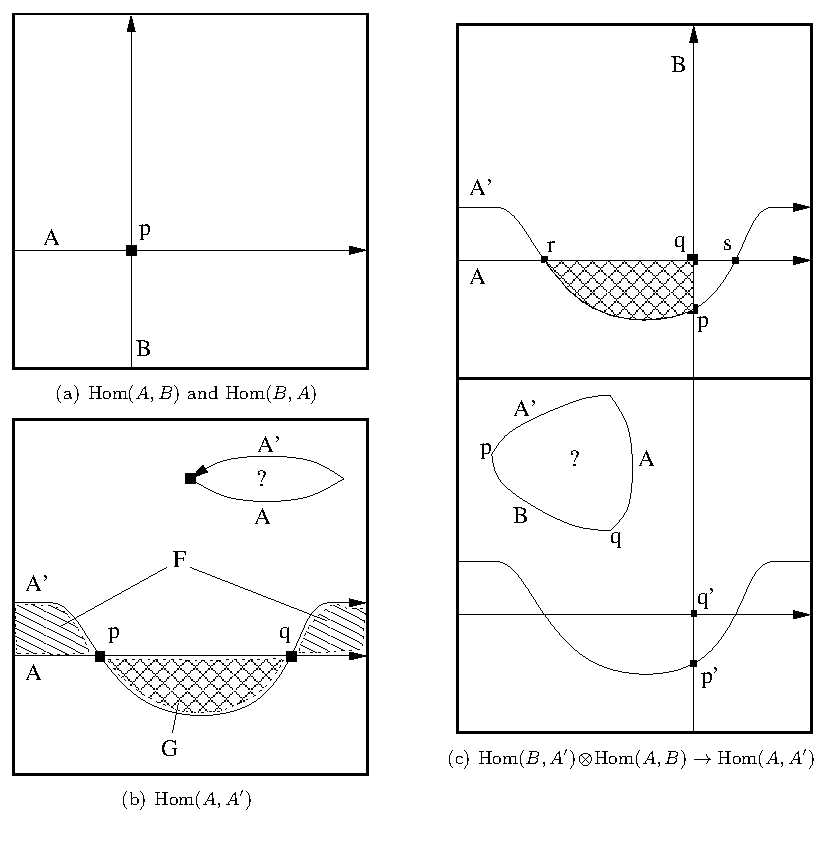
\includegraphics[width=0.95\linewidth]{figures/fig2.pdf}
  \caption{计算 Floer 链复形的图示：(a) $\mathrm{Hom}(A,B)$ 与 $\mathrm{Hom}(B,A)$；(b) $\mathrm{Hom}(A,A')$；(c) $\mathrm{Hom}(B,A')\otimes\mathrm{Hom}(A,B)\to\mathrm{Hom}(A,A')$。（原文 Figure 2，第 37 页）}
  \label{fig:floer-complex}
\end{figure}

接下来考虑 $\mathrm{Hom}(A,A)$。我们已由定理~\ref{thm:4.2} 知道它的上同调代数必同构于奇异上同调 $H^*(A,\Lambda_t)$，而后者是 $\Lambda_t\oplus\Lambda_t(-1)$（因为 $A$ 是圆周）。把 $A$ 作一个小的微扰、得到一条哈密顿同伦的曲线 $A'$ 来计算它，似乎更有启发性。这样的一个微扰如子图~\ref{fig:floer-complex}(b) 所示。我们看到 $\mathrm{Hom}(A,A')$ 是二维的，由 $p$ 与 $q$ 生成。又注意 $\tilde{s}_{A'}(p)=-\epsilon<0$，故 $\mu_p(A,A')=-[-\epsilon-0]=1$。相反地，$\tilde{s}_{A'}(q)=\epsilon>0$，故 $\mu_q(A,A')=0$。于是 $\mathrm{Hom}(A,A')$ 可能带有非零微分 $d(q)=\lambda p$。由第~\ref{subsec:fuk-surface} 小节对 Fukaya 范畴的描述，我们通过寻找以 $A$ 与 $A'$ 为边的浸入二边形（immersed bigon，模等价）来确定该微分。供参考，这类二边形的形状已画在图中。可以看出恰有两个这样的二边形，在图中标为 $F$ 与 $G$。于是
\[
dq=(t^F\pm t^G)p.
\]
这里的符号取决于我们尚未说明的约定。但注意必须有 $\mathrm{Hom}_{H\mathrm{Fuk}}(A,A')\neq0$，因为该集合中必有一个元素代表 $\mathbf{1}_A$。这只有在 $dq=0$ 时才能发生，而此时确实有 $\mathrm{Hom}_{H\mathrm{Fuk}}(A,A')\simeq H^*(A,\Lambda_t)$，与预期一致。还要注意 $dq=0$ 确实是可能的：微扰是哈密顿的，故 $F$ 与 $G$ 面积相同，于是若取上式的负号就有 $dq=0$。

% [Tutor Note: 易错点（Floer 微分符号与取向）：$dq=(t^F\pm t^G)p$ 的符号由曲线定向与圆盘的面积形式共同决定，原文未固定该约定。真正不依赖约定的是“$F$ 与 $G$ 面积相等”（微扰是哈密顿的，两条二边形面积相同），于是 $t^F=t^G$：取负号时两项相消得 $dq=0$；取正号则 $dq\ne0$，与 $\mathbf{1}_A\in\mathrm{Hom}_{H\mathrm{Fuk}}(A,A')$ 矛盾。换言之，$1_A$ 的存在性反过来定出了符号约定。]

对 $\mathrm{Hom}(B,B)$ 有类似的论证。于是我们发现，作为向量空间
\[
H(\mathcal{Q})\simeq Q
\]
（其中 $Q$ 仍是命题~\ref{prop:6.2} 中的代数）。与考察椭圆曲线的 Ext 代数时一样，几乎所有合成又都由形式理由确定；并且只要说明
\[
\mathrm{Hom}_{H\mathrm{Fuk}}(A,B)\,\mathrm{Hom}_{H\mathrm{Fuk}}(B,A)\neq0,
\qquad
\mathrm{Hom}_{H\mathrm{Fuk}}(B,A)\,\mathrm{Hom}_{H\mathrm{Fuk}}(A,B)\neq0,
\]
就能证明 $H(\mathcal{Q})\simeq Q$ 作为代数成立。也就是说，我们需要确定某个 $m_2$，即数一些三角形。现在考察子图~\ref{fig:floer-complex}(c)。我们将说明映射
\[
\mathrm{Hom}_{H\mathrm{Fuk}}(B,A')\otimes\mathrm{Hom}_{H\mathrm{Fuk}}(A,B)\longrightarrow
\mathrm{Hom}_{H\mathrm{Fuk}}(A,A')\simeq\mathrm{Hom}_{H\mathrm{Fuk}}(A,A)
\]
不是零映射。图中我们有两条经线 $A$ 与 $B$，以及 $A$ 的微扰 $A'$。为便于说明，我们画了表示环面的正方形的两份拷贝，把它们看作格 $\mathbb{Z}^2\subset\mathbb{R}^2$ 的两个基本域。在 $T$ 上，如前所述 $A$ 与 $B$ 有唯一交点，记为 $q$。点 $q'$ 与它等价。类似地，$A'$ 与 $B$ 交于唯一一点 $p$，图中还画出了另一个等价的交点 $p'$。又 $A'$ 与 $A$ 交于 $r$ 与 $s$。如前所述，我们确定 $|q|=0$、$|p|=1$、$|r|=1$、$|s|=0$。我们猜测
\[
m_2(p,q)=\lambda r,\qquad \lambda\neq0.
\]
（事实上，在 $B$ 与 $A'$ 的交点中，$r$ 是唯一具有正确次数的点。）正如第~\ref{subsec:fuk-surface} 小节所解释的，要计算这个乘积，需要数三角形。我们要找的三角形类型已画在图中：以 $q$、$p$ 和 $x$ 为顶点（按顺时针次序）、沿图中所示曲线段相连的三角形。图中我们还给一个这样的三角形画了阴影。

% [Tutor Note: 几何直观（多边形计数的面积权重）：$m_2$ 的三角形计数就是 Floer 复形中“两个交点合成第三个交点”的圆盘计数；在 $\Lambda_t$ 中每个圆盘以 $q^{\mathrm{area}}$ 加权（$q=e^{-t}$，面积越大权越小），因此只有面积相同的圆盘才会相消。这里 $y$ 坐标的单调性论证给出“唯一性”，避免了对全部格点平移求和的无穷计数——这正是环面的 Floer 同调能显式算出的根源。]

现在的主要观察是：在等价意义下这是唯一的这种三角形。也就是说，它是唯一以 $q$ 本身（而非某个等价点）为顶点的这种三角形。事实上，这种三角形的边 $q\to p$ 是 $y$ 坐标能改变超过 $1$ 的唯一一条边；即使沿另外两条边合起来，$y$ 坐标也绝不可能改变 $1$（因为另外两条边落在 $A$ 或 $A'$ 上）。但绕整个三角形一周必须使 $y$ 坐标不变，所以若它在某处改变超过 $1$，就必须改变两次，而这是不可能的。由此三角形的第二个顶点必须落在与我们出发时相同的基本域内，即它必须是 $p$。剩下的就简单了：三角形到 $T$ 的映射必须是保向的，且在角点之外是嵌入。于是三角形的第二条边必须“向左出发”（由定向决定），而第三个顶点必须是 $r$（而不是它的某个平移），否则我们无法得到嵌入。

另一个合成的处理与之完全相同，于是抽象镜像对称的证明到此完成。

% [Tutor Note: 记号提示：图~\ref{fig:floer-complex}(c) 中以“?”标出的那个顶点，正是正文所记的三角形第三个顶点 $x$；论证的结论是它必须等于 $r$（而不是 $r$ 的某个平移），故正文结尾说“第三个顶点必须是 $r$”。又，图 (c) 下半部分标出的 $q'$、$p'$ 是 $q$、$p$ 在相邻基本域中的等价点，对照画出的两份正方形即可看出平移关系。]
       % §6.2-6.3
% ============================================================
%  sec07.tex —— §7 椭圆曲线镜像对称的图示（原文 pp.38–44）
%  原文：Homological Mirror Symmetry for Elliptic Curves
%  外部交叉引用均按 GUIDE §6.5 的“原文编号” key：
%    thm:6.1, thm:6.4, thm:4.2, prop:2.5, thm:3.2,
%    subsec:maslov (4.3.2), subsec:6.3 (原文 “compare section 6.3”)
%  本节自身带编号的定理类：prop:7.1, thm:7.2, thm:7.3；
%  7.3 中原文不带编号的 Lemma 用 lemma*（不占计数，以保证 thm:7.3 编号正确）。
% ============================================================

\section{椭圆曲线镜像对称的图示}
\label{sec:illus}

\begin{keytakeaways}
  \item \textbf{物理/几何图像}：$T$ 中斜率为 $m/n$ 的测地圆在镜像下对应 $E$ 上秩 $n$、次数 $m$ 的向量丛；镜像曲线的方程由 $A$、$B$ 两条标准经线之间的多边形计数完全确定。
  \item \textbf{数学工具}：扭变函子 $T_B^{3n}$ 作用下的 Hom 空间给出射影坐标环，theta 级数 $A_i$、$B_i$ 给出结构常数，$j$-不变量由 Hesse 型三次方程的参数 $z$ 算出。
  \item \textbf{核心结论}：镜像曲线是 $\Lambda_t$ 上的光滑平面三次曲线，其 $j$-不变量等于经典 $j(q)$ 的 Laurent 展开（定理~\ref{thm:7.2}）；并且对任意 $C\in\Fuk(T)$ 有 $h(C)=k(\psi(C))$（定理~\ref{thm:7.3}）。
\end{keytakeaways}

本节我们打算收获此前为证明定理~\ref{thm:6.1} 与~\ref{thm:6.4} 所付出的全部努力。回忆我们已在其中证明：存在某个三次曲线 $E$，以及拟等价
\[
\psi\colon D^\pi\Fuk(T)\longrightarrow \Dinf(E).
\]
它由 $\psi(A)=\cO$ 与 $\psi(B)=\cO/P$ 确定，其中 $A$、$B$ 是标准经线（meridians）。

然而，我们并不知道 $E$ 是哪条曲线，甚至不知道它是否光滑。我们在第~\ref{subsec:determination}~小节解决这个问题。事实上，定理~\ref{thm:6.4} 还包含了确定 $E$ 的方法：从对应 $\cO$ 与 $\cO/P$ 的两条标准经线 $A$、$B$ 出发，考虑环
\[
S=\bigoplus_{n\ge 0}\Hom_{H^0D^\pi\Fuk(T)}\bigl(A,\,T_B^{3n}(A)\bigr).
\]
这是 $E$ 的射影坐标环。利用一些显式的多边形计数，我们可以求出 $E$ 的定义方程、验证它光滑，并计算其 $j$-不变量。

% [Tutor Note: 这里出现的指数是 $3n$ 而不是 $n$：$S$ 的第 $n$ 个分次片 $S_n=\Hom(A,T_B^{3n}(A))$ 的维数为 $3n$（$S_1$ 维数 3、$S_2$ 维数 6、$S_3$ 维数 9），恰好等于 $h^0(\cO_E(3n))=3n$。可把这个维数作为核对“$T_B^{3n}$ 对应 $\cO_E(3n)$ 的 Serre 扭转”这一对应关系的独立校验；若把指数误读成 $n$，则 $S_1$ 只有一维，无法给出三次曲线的三个齐次坐标。]

完成这些后，我们更细致地研究镜像对应 $\psi$。在第~\ref{subsec:rank-slope}~小节，我们定义向量丛的秩与斜率，并说明 $T$ 中斜率为 $m/n$ 的测地圆 $C$ 如何对应到镜像对应下它在 $\Dinf(E)$ 中所代表的向量丛的秩与斜率。

观察到群 $SL_2(\ZZ)$ 自然地作用在 $T$ 上，从而它（或更确切地说，它的中心扩张）作用在 $\Fuk(T)$ 上。由镜像对应，$\Dinf(E)$ 上必存在相应的作用。在第~\ref{subsec:braid}~小节我们构造这一作用，并用它证明上一小节草拟的秩与斜率对应。

\subsection{镜像曲线的确定}
\label{subsec:determination}

我们现在执行上面草拟的方法。为此，我们在 $T$ 的万有覆盖 $\RR^2$ 中工作。注意 $\rho(x,y)=(x,y+3x)$ 是 $\tau_B^3$ 的一个模型。令 $L_i=\rho^i(A)$。

% [Tutor Note: $\rho$ 是三次 Dehn 扭转 $\tau_B^3$ 在万有覆盖上的仿射模型，而不是 $\tau_B$ 本身——这正是“指数 3”的来源。核对时可在 $\RR^2/\ZZ^2$ 上看 $\rho$ 的线性部分 $\left(\begin{smallmatrix}1&0\\3&1\end{smallmatrix}\right)$：它的幂 $\rho^i$ 给出斜率为 $3i$ 的直线 $L_i$，即 $L_i=\rho^i(A)$。若误把 $\rho$ 当作一次扭转，则 $L_1$ 会是斜率为 1 的直线，与 $X_i=(i/3,0)$ 等交点坐标全部对不上。]

我们必须找到 $S_1=\Hom(A,L_1)$ 的（三个）生成元，以及它们在 $S_3=\Hom(A,L_3)$ 中满足的一个三次关系。为此，令 $X_i=(i/3,0)$（$i=0,1,2$），$Y_i=(i/6,0)$（$i=0,\ldots,5$），$Z_i=(i/9,0)$（$i=0,\ldots,8$）。这里以及别处，指标都按适当的 $n$ 作“$(\mathrm{mod}\ n)$”理解（例如对 $X_i$ 取 $n=3$）。注意 $\Hom(A,L_i)$ 是集中位于 $0$ 次、维数为 $3i$ 的分次向量空间。事实上，$X_i\in\Hom(A,L_1)$、$Y_i\in\Hom(A,L_2)$、$Z_i\in\Hom(A,L_3)$ 分别是这些向量空间（即交点）的自然生成元。

% [Tutor Note: 三组交点的分母不同并非笔误：$A$ 与 $L_i$（斜率 $3i$ 的直线）在基本域内恰有 $3i$ 个交点，所以 $X_i$ 分母为 3（3 个点）、$Y_i$ 分母为 6（6 个点）、$Z_i$ 分母为 9（9 个点）。所有 Hom 空间都集中在 0 次（无分次移位），因此后面三次关系的系数是纯数（theta 级数），不涉及 Koszul 符号。]

于是，我们需要做的是：把 $X_i$ 的十个三次单项式用 $\Hom(A,L_2)$ 的九个基元素 $Z_j$ 表示出来。这里必须回忆，$S$ 上的环结构是“经由 $\rho$”产生的。例如 $X_1X_2$ 指的是 $m_2(\rho(X_1),X_2)\in\Hom(A,L_2)$，其中我们把 $\rho(X_1)\in\Hom(\rho(A),\rho(L_1))=\Hom(L_1,L_2)$ 计算在内。

% [Tutor Note: 原文此处作“nine basis elements $Z_j$ of $\Hom(A,L_2)$”，但按上文 $Z_j\in\Hom(A,L_3)$、且 $\dim\Hom(A,L_3)=9$，这里应为 $\Hom(A,L_3)$。译文保留原文写法，见汇报中的原文疑误清单。]
% [Tutor Note: 这个“经由 $\rho$”的乘法是本节最容易出错的地方：复合 $m_2(\rho(X_1),X_2)$ 要求第一个因子的起点先被 $\rho$ 搬到 $L_1$，因此单调的“交换环”直觉在此失效，$A_{i-j}$、$B_{2j-i}$ 中指标的正负号与偏移（$+3$、$+6$、$+12$）都来自这个扭曲。算三次单项式前，务必先用已知的交换性、结合性核对 $X_iX_j=X_jX_i$。]

因此我们真正想做的是：先把 $X_i$ 的六个二次单项式用 $Y_j$ 表示，再由此算出三次单项式。这里我们用到了已知的事实：$S$ 必须是交换且结合的。

让我们看一个例子。假设要用 $Y_j$ 表示 $X_0^2$。于是我们要找顶点为 $X_0$、$\rho(X_0)=X_0$ 以及某个 $Y_j$ 的三角形。考虑图~\ref{fig:triangles}。

% [Tutor Note: 原文此处引用“figure 7.1”，但原书该图的实际编号是 Figure 3（第 40 页，本译本为图~\ref{fig:triangles}）。这是原文自身的编号不一致（正文用章节式编号，图题用全文连续编号）；译文正文按实际图编号引用，不再保留“7.1”这一不存在的图号。]

该图显示万有覆盖，其中所有点与曲线（直线）都无限次重复。图中用阴影标出的是我们要找的两个三角形 $F$ 与 $G$。容易看出，其余所有对 $X_0^2$ 有贡献的三角形都是这两个三角形的平移与伸缩。由此可得 $X_0^2=A_0Y_0+A_3Y_3$。我们来确定 $A_3$。这意味着要数 $F$ 的伸缩。容易看出，它们由整数 $n\in\ZZ$ 标号，顶点为 $(0,0)$、$(2n+1,6n+3)$ 与 $(0,n+1/2)$。图中所示的三角形 $F$ 对应 $n=0$。对应 $n$ 的三角形面积为
\[
\frac12\Bigl(n+\frac12\Bigr)(6n+3)=3\Bigl(n+\frac12\Bigr)^2 .
\]
因此
\[
A_3=\sum_{n\in\ZZ} t^{\,3(n+\frac12)^2}.
\]

% [Tutor Note: 这里的 $t$ 是 Novikov 变量，单项式 $t^{\text{面积}}$ 记录三角形的辛面积（相对于基本域面积归一化）。面积公式 $3(n+1/2)^2$ 是“底 $\times$ 高 $/2$”：竖直边长为 $n+1/2$、水平宽为 $6n+3$。面积对 $n\to -n-1$ 对称，这正是 theta 级数出现的原因；同时它解释了为什么 $A_3$ 只含半整数平移的项。]

这是一个经典的 theta 级数。事实证明，我们必须做的所有三角形计数都给出这类级数。Zaslow \cite{ref24} 详细完成了这些计数。他的结果可概括如下。记
\[
A_i=\sum_{n\in\ZZ} t^{\,3(n+\frac{i}{6})^2},
\qquad
B_i=\sum_{n\in\ZZ} t^{\,9(n+\frac{i}{18})^2}.
\]
则
\[
\begin{aligned}
X_iX_j &= A_{i-j}Y_{i+j}+A_{i-j+3}Y_{i+j+3},\\
Y_iX_j &= B_{2j-i}Z_{i+j}+B_{2j-i+6}Z_{i+j+3}+B_{2j-i+12}Z_{i+j+6}.
\end{aligned}
\]

由此，求出三次单项式之间的线性关系完全是例行公事，尽管相当繁琐。由它可以计算镜像的 $j$-不变量。结果如下。

\begin{proposition}[Zaslow]\label{prop:7.1}
令
\[
u=A_2B_0+A_1B_9,\qquad p=A_0B_0+A_3B_9,\qquad q=A_0B_6+A_3B_3,\qquad z=\frac{2q+p}{3u}.
\]
则 $X_i$ 满足的三次关系为
\[
X_0^3+X_1^3+X_2^3-3z\,X_0X_1X_2=0.
\]
这是一条光滑三次曲线，其 $j$-不变量为
\[
j_{\Fuk}=-27\,\frac{z^3(z^3+8)^3}{(1-z^3)^3}.
\]
\end{proposition}

% [Tutor Note: 作者写“working out the linear relation ... is entirely routine”，省略的实质是：$S_3=\Hom(A,L_3)$ 是 9 维空间，而 $X_i$ 的三次单项式有 $\binom{5}{3}=10$ 个，故必存在唯一（差一个标量）的线性关系；$S$ 的交换性把它对称化为 $X_0^3+X_1^3+X_2^3-3zX_0X_1X_2=0$，参数 $z$ 由代入 $A_i,B_i$ 的显式 theta 级数确定。实际计算顺序是：先用 $A_i$ 把六个二次单项式写成 $Y_j$ 的组合，再用 $B_i$ 把 $Y_jX_k$ 写成 $Z_l$ 的组合，最后消去 $Y$、$Z$。]
% [Tutor Note: 核对 $j$-不变量时注意参数约定：Hesse 型三次曲线 $X^3+Y^3+Z^3-3zXYZ=0$ 的 $j$-不变量为 $-27z^3(z^3+8)^3/(1-z^3)^3$；经典模 lambda 函数公式是 $j=256(1-\lambda+\lambda^2)^3/[\lambda^2(1-\lambda)^2]$。$z$ 与 $\lambda$ 之间是分式线性变换（Hesse 参数与 Legendre 参数），不可直接令 $z=\lambda$ 或 $z^3=\lambda$。建议用两个特殊值锚定归一化：$j(i)=1728$，$j(e^{2\pi i/3})=0$。另注意原文在此把 $j$-不变量记作 $j_{\Fuk}$ 以区别于经典 $j$。]

这完全回答了本小节提出的问题。此外，Zaslow 观察到，在我们呈现镜像对称的方式下，出现了一个小小的奇迹。考虑上半平面中的 $\tau$，以及复环面 $E_\tau=\CC/\ZZ\oplus\tau\ZZ$。这是一条椭圆曲线，其 $j$-不变量是经典函数。它通常用 $q=e^{2\pi i\tau}$ 写出，因为此时它具有整系数的 Laurent 级数展开 \cite{ref13}：
\[
j(q)=\frac1q+744+196884q+\ldots
\]

% [Tutor Note: 原文排印为 $E_\tau=\CC/\ZZ\oplus\tau\ZZ$；按数学含义应读作 $\CC/(\ZZ\oplus\tau\ZZ)$（斜杠只作用于整个格）。这是原文的一处排印歧义，译文保留原式并在此标注。]
% [Tutor Note: 指数约定必须核对：$q=e^{2\pi i\tau}$（不是 $e^{\pi i\tau}$），于是 $j(q)=q^{-1}+744+196884q+\cdots$，其中 196884 是 Monster 表示维数（McKay 观察）。若换成 $Q=e^{\pi i\tau}$ 的约定，展开式会变成 $Q^{-2}+\cdots$，系数完全不同。后文镜像映射把形式变量 $t$ 与 $q$ 等同起来，这个替换的逐阶验证正是定理~\ref{thm:7.2} 的内容。]

% 图 3 原位于第 40 页顶部；正文在 7.1 开头引用它（原文误作“figure 7.1”）。fig3.pdf 已按整幅图重新裁剪。
\begin{figure}[htbp]
  \centering
  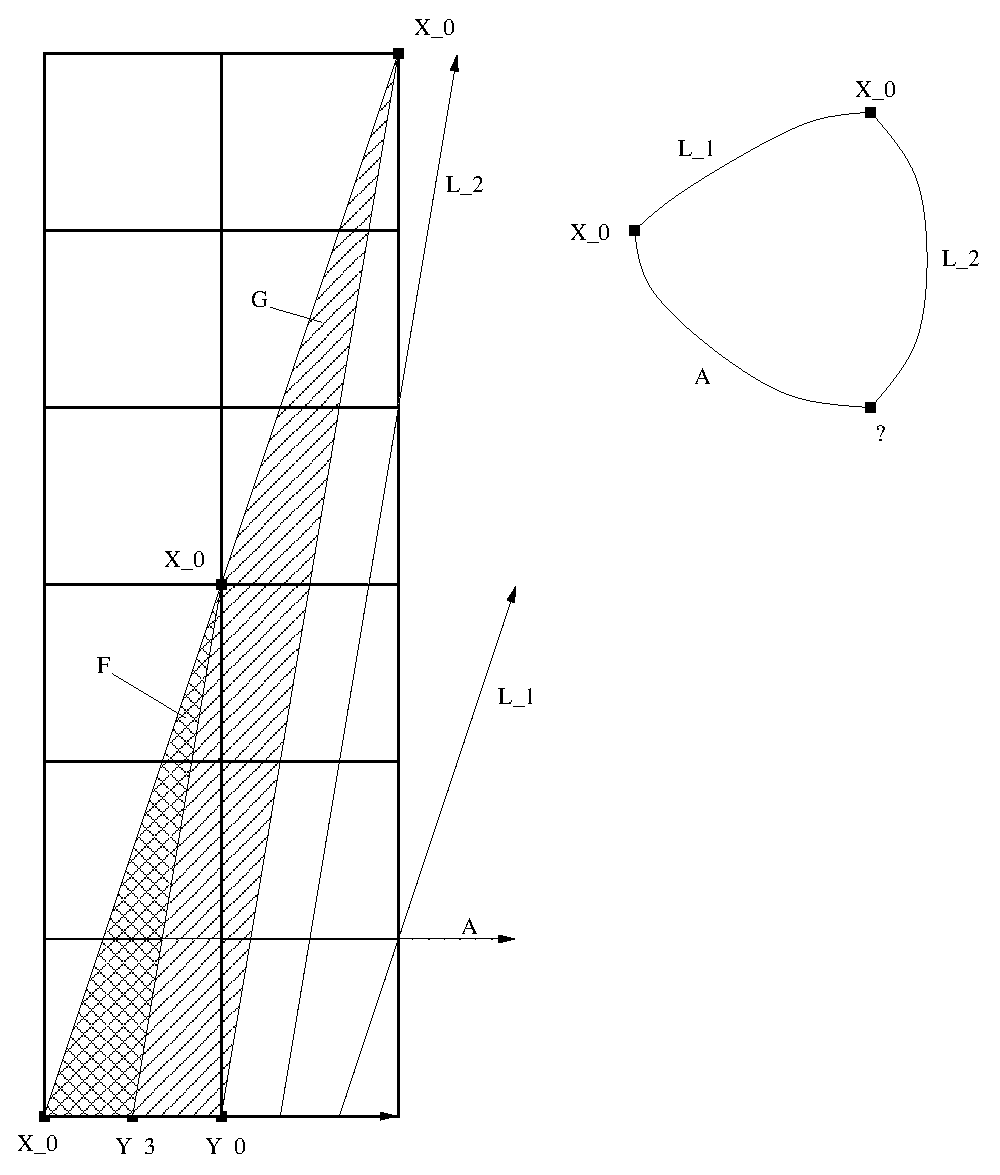
\includegraphics[width=0.95\linewidth]{figures/fig3.pdf}
  \caption{对 $X_0^2$ 有贡献的部分三角形。左图为 $T$ 的万有覆盖：网格、直线 $A$、$L_1$、$L_2$，标记点 $X_0$、$Y_0$、$Y_3$，以及用阴影标出的三角形 $F$ 与 $G$；右图为环面上由曲线段 $A$、$L_1$、$L_2$ 围成的三角形，两个顶点标为 $X_0$，第三个顶点标为“？”。（原文 Figure 3，第 40 页）}
  \label{fig:triangles}
\end{figure}

\begin{theorem}\label{thm:7.2}
$T$ 的镜像曲线是 $\Lambda_t$ 上的光滑平面三次曲线，其 $j$-不变量 $j$ 由经典 $j(t)$ 函数的 Laurent 展开给出。
\end{theorem}

% [Tutor Note: 这个定理的“证明”被作者略去了。作者在下一段说原则上可以证明 $j_{\Fuk}(t)$ 是模函数、再比较有限维空间中的前几项；实际需要验证的是 $j_{\Fuk}$ 在 $SL_2(\ZZ)$（或某个同余子群）下的变换性质，这是 Zaslow \cite{ref24} 的 theta 级数计算的核心，属于“非平凡”的部分。作者随后用 $O(q^4)$ 的逐阶验证代替证明，这一点务必在引用定理时说明。]

原则上，可以通过证明 $j_{\Fuk}(t)$ 是模函数、再计算级数展开的前几项来证明这一点（因为模函数空间是有限维的）。然而，这相当不平凡。我们转而满足于逐阶验证该断言，想要多少项就验证多少项（这当然不是证明，但仍颇具说服力）：附录中图~\ref{fig:series-py} 的 Python 脚本 \texttt{series.py} 可用于计算 $j_{\Fuk}(t)$ 的级数展开到任意所需阶数。它通过暴力计算进行，即先把 $j_{\Fuk}(t)$ 中出现的 theta 函数计算到足够高的阶数，然后求逆并相乘。我们已用它验证该断言直到 $O(q^4)$。

\subsubsection*{$\CC$ 上的镜像对称}

一个有趣的观察是：给定上半平面中的一个复数 $q$，可以构造一个 $A_\infty$-范畴 $\Fuk_q(T)$，它由 $\Fuk(T)$ 通过把 $t$“替换”为 $q$ 得到。也就是说，定义中相应的级数实际上收敛。上述结果于是表明：若 $E$ 是 $\CC$ 上一条 $j$-不变量为 $j(q)$（对某个特定的 $q\in\CC$）的椭圆曲线，则 $\Dinf(X)$ 与 $D^\pi\Fuk_q(T)$ 拟等价。因此，在 $\CC$ 上，我们为所有椭圆曲线找到了镜像。

% [Tutor Note: 原文此处有两处容易误导的地方。其一，“given a complex number $q$ in the upper half plane”中的 $q$ 应为模参数 $\tau\in\mathbb{H}$（$q=e^{2\pi i\tau}$ 并不在上半平面）；这是原文的笔误，译文保留原词并在此标注。其二，结论中的 $\Dinf(X)$ 按上下文应为 $\Dinf(E)$（$E$ 才是被镜像的椭圆曲线，本节从未定义过 $X$）；同样保留原文并标注。理解时按“$\tau\in\mathbb{H}$，$\Dinf(E)\simeq D^\pi\Fuk_q(T)$”读即可。]

\subsection{图示的镜像对称：向量丛的秩与斜率}
\label{subsec:rank-slope}

我们的镜像对称证明相当抽象。特别地，确定嵌入圆 $C\in\Fuk(T)$ 在镜像对应下的像 $\psi(C)$ 绝非平凡。这里我们至少希望描述 $\psi(C)$ 是何种对象。事实上，可以证明它总是（某个平移下的）局部自由层或摩天楼层，因此一个非常自然的问题是：$\psi(C)$ 具有怎样的秩与第一陈类。这就是本小节要处理的问题。

设 $\cA$ 是三角 $A_\infty$-范畴，$B$ 是阿贝尔群。若对 $\cA$ 中任意态射 $f\colon X\to Y$ 都有
\[
0=e(X)-e(Y)+e(\operatorname{cone}(f)),
\]
则称映射 $e\colon\Ob(\cA)\to B$ 为欧拉示性数（或加性函数）。显然，$e$ 由它在 $\cA$ 的任意一组生成元（而不必是分裂生成元）上的取值确定。例如，若 $\cA=\Dinf(X)$、$X$ 是光滑射影簇，则 $e$ 由它在向量丛上的取值确定（由定理~\ref{thm:3.2}，这些向量丛是生成元）。

% [Tutor Note: 欧拉示性数的定义等价于“在正合三角形上可加”：由 $X\to Y\to\operatorname{cone}(f)\to$ 得 $e(X)-e(Y)+e(\operatorname{cone}f)=0$，故 $e$ 是三角范畴上的加性函数。注意“生成元”与“分裂生成元（split-generators）”的区别：这里只要求生成元，是因为 $e$ 在三角范畴上可加、自动沿分裂闭包延拓；若换成一般的加法不变量，可能只由分裂生成元决定。此外 $e$ 必在平移下变号：$e(X[1])=-e(X)$。]

设 $\cA$ 是 $k$ 上的三角 $A_\infty$-范畴，$X\in\cA$ 具有有限上同调维数，即：对任意 $Y\in\cA$ 存在 $n$，使得对所有 $|r|>n$ 有 $H^r\Hom_{\cA}(X,Y)=0$，并且对所有 $r$ 有 $\dim_k H^r\Hom_{\cA}(X,Y)<\infty$。此时
\[
e(Y)=\sum_i(-1)^i\dim_k H^i\Hom_{\cA}(X,Y)=:\chi\bigl(H^*\Hom(X,Y)\bigr)
\]
是 $\cA$ 上的欧拉示性数。这来自 $H^0\cA$ 是三角范畴这一事实。对 $\Hom(\bullet,X)$ 有类似结果。

现在设 $X$ 是光滑射影簇，$P\in X$ 是闭点。我们在 $\Dinf(X)$ 上定义两个欧拉示性数，称为秩与斜率：
\[
\operatorname{rk}(\cF)=\chi\bigl(\Ext^*(\cF,\cO_X/P)\bigr),
\qquad
\operatorname{sl}(\cF)=\chi\bigl(\Ext^*(\cO,\cF)\bigr)=\chi\bigl(H^*(X,\cF)\bigr).
\]
容易看出，对局部自由层，这个秩的定义与通常的定义一致，从而特别地不依赖于 $P$ 的选取。又若 $X$ 是椭圆曲线、$\cL$ 是线丛，则由 Riemann--Roch 定理与 Serre 对偶，$\cL$ 的斜率等于其次数（即第一陈类）。\footnote{可以证明第一陈类 $c_1$ 也是欧拉示性数。若 $X$ 不是椭圆曲线，这或许是比我们的定义更好的斜率定义。由于我们只处理椭圆曲线，我们将忽略这个问题。}

% [Tutor Note: 秩的定义用 $\cO_X/P$（摩天楼层）而不是 $\cO_X$：$\chi(\Ext^*(\cF,\cO_X/P))$ 数的是 $\cF$ 在 $P$ 处的纤维维数，对局部自由层恰好等于秩，且与 $P$ 无关；斜率则用 $\cO$ 配对，$\chi(\Ext^*(\cO,\cF))=\chi(H^*(X,\cF))$，对线丛由 Hirzebruch--Riemann--Roch 得 $\deg$。核对时注意 $\Ext^*$ 指全 Ext 复形（带分次），$\chi$ 是交错和而不是 $\dim\Hom$。]

当然，我们可以把这两个欧拉示性数组合起来，得到映射
\[
k\colon \Dinf(E)\to\ZZ^2,\qquad \cF\mapsto\bigl(\operatorname{sl}(\cF),\operatorname{rk}(\cF)\bigr).
\]
在镜像对称下，它对应映射 $k'\colon\Fuk(T)\to\ZZ^2$，由相同的公式定义。

还有另一个来自几何的、形式类似的映射，从 $\Fuk(T)$ 出发。即回忆 $\Fuk(T)$ 的对象（不是 $D^\pi\Fuk(T)$ 的对象）由带额外数据的嵌入圆表示。于是我们有映射
\[
h\colon \Fuk(T)\to H_2(T)\simeq\ZZ^2.
\]
具体地，若曲线 $C$ 在 $T$ 的万有覆盖中由斜率为 $m/n$ 的直线表示（并且“朝右”定向），其中分式已约至最简且 $n>0$，则 $h(C)=(m,n)$。这就解释了“斜率”一词。

% [Tutor Note: 几何直观：$h$ 把拉格朗日圆周送到它的同调类；在万有覆盖中取斜率为 $m/n$ 的直线，$m,n$ 就是它相对于标准经线 $A,B$ 的同调系数。镜像一侧的 $(\operatorname{sl},\operatorname{rk})=(m,n)$ 意味着“斜率 $m/n$”在代数侧应读作“次数/秩”。作者把 $h$ 与 $k'$ 都取成二元组，正是为了让 $SL_2(\ZZ)$ 的线性作用两边一致；注意 $k$ 的分量次序是（斜率，秩），与 $h$ 的（$m,n$）次序相同，不要颠倒。]
% [Tutor Note: “oriented to the right”与 $n>0$ 的约定是固定符号的关键：同一条无向直线有两种定向，取 $n>0$ 的定向消除这个二义性，否则 $h(C)$ 会差一个整体符号 $(m,n)\mapsto(-m,-n)$。$SL_2(\ZZ)$ 作用正是以这种方式把不同的 $(m,n)$ 联系起来。]

我们断言 $h=k'$（在有定义处）。这用手检查并不特别困难。这里我们验证 $h(C_x)=k'(C_x)$，其中 $C_x$ 是对应于平行于 $A$ 的直线
\[
\{(t,x)\mid t\in[0,1]\}
\]
的曲线。一般情形将在下一小节建立。若 $x=0$，断言是清楚的：因为 $C_0=A$，而 $\psi(A)=\cO$ 的秩为 1、斜率（即次数）为 0。此外，若 $x\ne 0$，则 $\Hom_{\Fuk(T)}(A,C_x)=0$（因为没有交点），故
\[
\operatorname{sl}'(C_x)=\chi(H^*\Hom_{\Fuk(T)}(A,C_x)=0.
\]
另一方面，$\Hom_{\Fuk(T)}(C_x,B)$ 是一维的、在 $0$ 次生成，且由与 $t=0$ 时完全相同的图像给出，因此 $\operatorname{rk}'(C_x)=1$。

% [Tutor Note: 原文此式缺少一个右括号：按上下文应为 $\operatorname{sl}'(C_x)=\chi(H^*\Hom_{\Fuk(T)}(A,C_x))=0$。译文保留原文写法，见汇报中的原文疑误清单。]
% [Tutor Note: 这里 $C_x$ 是平行于 $A$ 的测地圆；$x\ne0$ 时它与 $A$ 无交点，故 $\Ext^*(A,C_x)=0$，斜率（次数）为 0；而它与 $B$ 恰好交于一点（在 0 次），故秩为 1。这与 $h(C_x)=(0,1)$ 一致。注意 $t=0$ 时 $C_0=A$，三个映射同时退化，作者用这个极限情形锚定符号。]

\subsection{辫作用}
\label{subsec:braid}

群 $SL_2(\ZZ)$ 自然地作用在 $T$ 上。它显然保持辛形式（因为行列式为 1 的矩阵保持体积），因此由第~\ref{subsec:maslov}~小节的讨论，它的所有元素都是可分次的。事实上众所周知，$SL_2(\ZZ)$ 由标准线性 Dehn 扭转 $M_A$ 与 $M_B$ 生成（比较第~\ref{subsec:6.3}~小节），并满足两个关系
\[
(M_AM_B)^6=\mathbf{1}
\qquad\text{与}\qquad
M_AM_BM_A=M_BM_AM_B.
\]
记 $s_1=\tilde{\tau}_A$ 与 $s_2=\tilde{\tau}_B$ 为这些 Dehn 扭转的标准分级。于是
\[
(s_1s_2)^6=\mathbf{1}[k_1],
\qquad
s_1s_2s_1=s_2s_1s_2[k_2].
\]
容易验证 $M_A$、$M_B$ 与 $M_AM_B$ 都把其自变量旋转一个小的正角度。由此观察容易看出 $k_1\ne 0$ 且 $k_2=0$。（其实容易验证 $k_1=2$，但我们并不真正需要这一点。）因此，由 $s_1$ 与 $s_2$ 生成的 $\mathrm{Sym}^{gr}(T)$ 的子群同构于辫群
\[
B_3=\langle s_1,s_2\mid s_1s_2s_1=s_2s_1s_2\rangle.
\]

% [Tutor Note: 这是本节的第一个关键点，也是最易混淆的地方。$SL_2(\ZZ)$ 是映射类群 $\mathrm{MCG}(T)$，由 $M_A,M_B$ 生成，满足 $(M_AM_B)^6=\mathbf{1}$ 与辫关系；但分次提升 $s_1,s_2$ 只满足“带平移”的 $(s_1s_2)^6=\mathbf{1}[k_1]$，其中 $k_1=2$ 是 Maslov 平移（$(M_AM_B)^6$ 的总旋转角为 $2\pi$ 而非 0）。$k_2=0$ 表明辫关系在两个分次提升之间精确成立。于是分次提升生成的是 $B_3$ 而不是 $SL_2(\ZZ)$：$B_3\twoheadrightarrow SL_2(\ZZ)$ 是满同态，核由 $(s_1s_2)^6$ 生成（$B_3$ 的中心由 $(s_1s_2)^3$ 生成，它在 $SL_2(\ZZ)$ 中的像是 $-\mathbf{1}$，阶为 2）。不要把辫关系 $s_1s_2s_1=s_2s_1s_2$ 与 $SL_2(\ZZ)$ 的 $(M_AM_B)^3=-\mathbf{1}$ 混为一谈，也不要把 $[k_1]$ 当作无意义的记号丢掉。]
% [Tutor Note: 作者说“$M_A$、$M_B$、$M_AM_B$ 都把其自变量旋转一个小的正角度”，省去的核对是：对每个映射追踪一个切向量的 Maslov 相位（即分次提升相对于未提升的偏移），三个元素引起的平移均为正；由此 $(M_AM_B)^6$ 的总平移为 $k_1=2$（转一整圈对应 Maslov 指标 2），而辫关系两边对应的平移相同，故 $k_2=0$。若按未分级的映射类群理解，会误以为 $k_1=k_2=0$，从而得不到辫群。]

这样我们就找到了 $\Fuk(T)$ 上的一个辫作用。通过镜像对应 $\psi$，这也在 $\Dinf(E)$ 上给出一个辫作用（回忆 $A_\infty$-范畴的拟等价具有拟逆）。

我们可以直接在 $\Dinf(E)$ 上构造这一作用。事实上，由总结 Fukaya 范畴性质的定理~\ref{thm:4.2}，$s_1$ 通过 $T_A$ 作用在 $\Fuk(T)$ 上，类似地 $s_2$ 通过 $T_B$ 作用。于是由定理~\ref{prop:2.5}（它说明扭变函子在 $A_\infty$-函子下保持）可知，在 $\psi$ 下，$s_1$ 的作用通过 $T_{\psi(A)}=T_{\cO}$ 给出，$s_2$ 的作用通过 $T_{\cO/P}$ 给出。仅此一点就已经相当有趣，因为先验地完全不清楚这些扭转是否可逆（尽管这一点可由“球状对象”理论推出）。

\subsubsection*{$h$ 与 $k$ 的比较}

我们现在利用这一辫作用来证明：对任意 $C\in\Fuk(T)$，有 $h(C)=k(\psi(C))$。

% [Tutor Note: 原文此句作“for and $C\in\Fuk(T)$”，疑为“for any $C$”之误；译文按“对任意 $C$”处理，见汇报中的原文疑误清单。]

\begin{lemma*}
设 $C\in\Fuk(T)$、$\cF\in\Dinf(E)$、$s\in B_3$，则
\[
h(sC)=s\,h(C),
\qquad
k(s\cF)=s\,k(\cF),
\]
其中 $\ZZ^2$ 上的作用经由自然的商映射 $SL_2(\ZZ)$ 给出。
\end{lemma*}

\begin{proof}
只需对 $s=s_1$ 与 $s=s_2$ 证明（因为它们生成 $B_3$），它们分别在 $\ZZ^2$ 上通过 $M_{\tau_A}$ 与 $M_{\tau_B}$ 作用。在辛侧，它们分别对应 $\tilde{\tau}_A$ 与 $\tilde{\tau}_B$；在代数侧，它们分别对应 $T_{\cO}$ 与 $T_{\cO/P}$。因此我们需要证明
\[
h(\tilde{\tau}_AC)=M_{\tau_A}h(C),\qquad C\in\Fuk,
\]
等等。

这在辛侧（即对 $h$）是显然的。在代数侧，我们只需观察由扭变函子定义给出的正合三角形
\[
\begin{aligned}
\cO\otimes\Ext^*(\cO,\cF)&\longrightarrow\cF\longrightarrow T_{\cO}(\cF)\longrightarrow\\
\cO/P\otimes\Ext^*(\cO/P,\cF)&\longrightarrow\cF\longrightarrow T_{\cO/P}(\cF)\longrightarrow .
\end{aligned}
\]
由于 $\operatorname{sl}$ 与 $\operatorname{rk}$ 是欧拉示性数，可得
\[
\begin{aligned}
\operatorname{sl}(T_{\cO}(\cF))
&=\operatorname{sl}(\cF)-\operatorname{sl}\bigl(\cO\otimes\Ext^*(\cO,\cF)\bigr)
=\operatorname{sl}(\cF),\\
\operatorname{rk}(T_{\cO}(\cF))
&=\operatorname{rk}(\cF)-\operatorname{rk}\bigl(\cO\otimes\Ext^*(\cO,\cF)\bigr)\\
&=\operatorname{rk}(\cF)-\chi\bigl(\Ext^*(\cO,\cF)\bigr)
=\operatorname{rk}(\cF)-\operatorname{sl}(\cF),\\
\operatorname{sl}(T_{\cO/P}(\cF))
&=\operatorname{sl}(\cF)-\operatorname{sl}\bigl(\cO/P\otimes\Ext^*(\cO/P,\cF)\bigr)
=\operatorname{sl}(\cF)-\chi\bigl(\Ext^*(\cO/P,\cF)\bigr),\\
\operatorname{rk}(T_{\cO/P}(\cF))
&=\operatorname{rk}(\cF)-\operatorname{rk}\bigl(\cO/P\otimes\Ext^*(\cO/P,\cF)\bigr)
=\operatorname{rk}(\cF).
\end{aligned}
\]
这里我们用到欧拉示性数是加性的、在平移下变号，以及 $k(\cO)=(0,1)$、$k(\cO/P)=(1,0)$。

% [Tutor Note: 这几行是本节符号最密集的地方。核对要点：(1) $\operatorname{rk}(\cO\otimes\Ext^*(\cO,\cF))=\chi(\Ext^*(\cO,\cF))=\operatorname{sl}(\cF)$，因为对线丛（这里是 $\cO$）取张量不改变 $\Ext$ 的维数结构；(2) 平移使欧拉示性数变号，故用“减去”而不是“加上”；(3) $k(\cO)=(0,1)$ 表示 $\cO$ 的（斜率，秩）为 $(0,1)$，$k(\cO/P)=(1,0)$ 同理；(4) 得到 $\operatorname{rk}(T_{\cO}(\cF))=\operatorname{rk}(\cF)-\operatorname{sl}(\cF)$ 后，回代到 $h$ 的公式即得 $M_{\tau_A}$ 对 $(m,n)$ 的作用矩阵，可与辛侧的旋转矩阵逐项比对。]

剩下要证明 $\chi(\Ext^*(\cO/P,\cF))=-\operatorname{rk}(\cF)$，并且像往常一样，只需对向量丛证明。一个简单的办法是考虑正合三角形 $\cO\to\cO(P)\to\cO/P$。若记 $e(\cF,\cG)=\chi(\Ext^*(\cF,\cG))$，则得到
\[
\begin{aligned}
e(\cO/P,\cF)
&=e(\cO(P),\cF)-e(\cO,\cF)\\
&=e(\cF^\vee,\cO(-P))-e(\cF^\vee,\cO)\\
&=-e(\cF^\vee,\cO/P)
\end{aligned}
\]
（第二行中我们两次用到 $\Ext^*(\cF\otimes\cL,\cG)=\Ext^*(\cF,\cG\otimes\cL^\vee)$）。但最后一个表达式正是 $-\operatorname{rk}(\cF^\vee)=-\operatorname{rk}(\cF)$。证毕。
\end{proof}

% [Tutor Note: 作者写“as usual it suffices to show this for vector bundles”，省略的是：$\Ext^*$ 与 Euler 示性数在正合三角形上可加，而 $\Dinf(E)$ 由向量丛生成（定理~\ref{thm:3.2}），故只需在生成元上验证；线丛情形由 Riemann--Roch 立得。第二步用到的 Serre 对偶为 $\Ext^i(\cF\otimes\cL,\cG)\cong\Ext^i(\cF,\cG\otimes\cL^\vee)$，以及 $\Ext^*(\cF^\vee,\cO)\cong H^*(X,\cF)$。]

\begin{theorem}\label{thm:7.3}
对任意 $C\in\Fuk(T)$，有
\[
h(C)=k(\psi(C)).
\]
\end{theorem}

\begin{proof}
众所周知，$SL_2(\ZZ)$ 在 $\ZZ^2$ 的形如
\[
Z_r=\{(m,n)\mid \gcd(m,n)=r\}
\]
的子集上传递地作用（这本质上是欧几里得算法的重述）。因此由引理，我们可以只考虑满足 $h(C)=(r,0)$ 的曲线 $C$。回忆可缩曲线不可分次（比较第~\ref{subsec:maslov}~小节），故知 $r>0$。我们实际上将证明 $r=1$ 是唯一可能。

一个用到平均曲率流理论 \cite{ref6} 的论证（因篇幅所限我们不得不省略）表明：若 $r=1$，则任何这样的曲线 $C$ 都哈密顿同伦于一条测地线 $C'$。$T$ 的测地线对应万有覆盖中的直线（具有有理斜率），而我们已经描述过 $h$ 在这类曲线上的作用。由此可知 $C'=C_x$（对某个 $x$，按第~\ref{subsec:rank-slope}~小节的记号）。但这正是我们在那里已经验证过的情形。

% [Tutor Note: 被省略的平均曲率流论证（Grayson \cite{ref6}）的实质是：在给定的 Hamiltonian 同伦类中，曲线缩短流收敛到一条测地线；$r=1$ 保证极限不自交（否则极限会是多重覆盖的圆，对应 $r>1$）。这是本节唯一用到分析的地方，也是“$r>0$”与“嵌入”假设发挥作用的地方。若想补全证明，需要 Grayson 的“Shortening embedded curves”中关于嵌入曲线在流下保持嵌入、并收敛到闭测地线的定理。]

若 $r>1$，我们仍可应用平均曲率流，找到一条曲率任意小的哈密顿同伦曲线 $C'$。但这样一条（曲率很小的）曲线必然自交。由于平均曲率流不产生自交，我们得出 $C$ 本来就有自交，而这是不允许的（我们要求曲线是嵌入的）。证毕。
\end{proof}

% [Tutor Note: “$r>1$ 时小曲率曲线必自交”的直观：若同调类为 $r$ 倍本原类，则曲线在 $T$ 上的投影至少绕 $r$ 圈；曲率很小时它近似一条斜率 $m/n$ 的直线，但 $m,n$ 有公因子 $r>1$，故必须回到自身附近，从而产生自交。这正是 $r=1$ 与 $r>1$ 的分界，也是“映射类群在 $Z_1$ 上传递”这一 Euclid 算法论证能把问题归约到 $(1,0)$ 的原因。]
        % §7 Illustrations

% ------------------------------ 参考文献 ------------------------------
% ============================================================
%  refs.tex —— 参考文献（原文 pp.44–45，共 24 条）
%  按原文样式保留英文，仅修复 PDF 抽取造成的连字与变音符：
%  fi/ff 连字展开、变音符写成 \"a 等；[12] 作者 Yank{\i} 用无点 i。
%  \bibitem 顺序即编号 [1]–[24]，不要插入 DOI。
% ============================================================

\begin{thebibliography}{99}

\bibitem{ref1} Mohammed Abouzaid. On the fukaya categories of higher genus surfaces. \emph{Advances in Mathematics}, 217(3):1192 -- 1235, 2008.

\bibitem{ref2} Sylvain E. Cappell, Ronnie Lee, and Edward Y. Miller. On the maslov index. \emph{Communications on Pure and Applied Mathematics}, 47(2):121--186, 1994.

\bibitem{ref3} David A Cox and Sheldon Katz. \emph{Mirror symmetry and algebraic geometry}. Math. Surveys Mono. AMS, Rhode Island, NJ, 1999.

\bibitem{ref4} Ana Cannas da Silva. Symplectic geometry. In F.J.E. Dillen and L.C.A. Verstraelen, editors, \emph{Handbook of Differential Geometry}. Elsevier, 2005.

\bibitem{ref5} Alice Fialowski and Michael Penkava. Deformation theory of infinity algebras. \emph{Journal of Algebra}, 255(1):59 -- 88, 2002.

\bibitem{ref6} Matthew A. Grayson. Shortening embedded curves. \emph{Annals of Mathematics}, 129(1):pp. 71--111, 1989.

\bibitem{ref7} Dieter Happel. Hochschild cohomology of finite--dimensional algebras. In Marie-Paule Malliavin, editor, \emph{S\'eminaire d'Alg\`ebre Paul Dubreil et Marie-Paul Malliavin}, volume 1404 of \emph{Lecture Notes in Mathematics}, pages 108--126. Springer Berlin Heidelberg, 1989.

\bibitem{ref8} Robin Hartshorne. \emph{Algebraic geometry}. Springer-Verlag, New York, 1977. Graduate Texts in Mathematics, No. 52.

\bibitem{ref9} Bernhard Keller. Introduction to A-infinity algebras and modules., 2001.

\bibitem{ref10} Maxim Kontsevich. Homological algebra of mirror symmetry. In \emph{Proceedings of the International Congress of Mathematicians}, pages 120--139. Birkh\"auser, 1994.

\bibitem{ref11} Yanki Lekili and Timothy Perutz. Arithmetic mirror symmetry for the 2-torus, 2012. Preprint.

\bibitem{ref12} Yank{\i} Lekili and Timothy Perutz. Fukaya categories of the torus and dehn surgery. \emph{Proceedings of the National Academy of Sciences}, 108(20):8106--8113, 2011.

\bibitem{ref13} James S. Milne. \emph{Modular Functions and Modular Forms}. 2009. Available at www.jmilne.org/math/.

\bibitem{ref14} Alexander Polishchuk. Massey and fukaya products on elliptic curves, 1998.

\bibitem{ref15} Alexander Polishchuk. Homological mirror symmetry with higher products, 1999.

\bibitem{ref16} Alexander Polishchuk. A-infinity structures on an elliptic curve. Commun.Math.Phys. 247 (2004) 527-551, 2004.

\bibitem{ref17} Alexander Polishchuk and Eric Zaslow. Categorical mirror symmetry: The elliptic curve. Adv.Theor.Math.Phys.2:443-470,1998, 1998.

\bibitem{ref18} Paul Seidel. Graded lagrangian submanifolds. \emph{Bulletin de la Soci\'et\'e Math\'ematique de France}, 128(1):103--149, 2000.

\bibitem{ref19} Paul Seidel. Homological mirror symmetry for the quartic surface, 2003.

\bibitem{ref20} Paul Seidel. \emph{Fukaya categories and Picard-Lefschetz theory}. Zurich lectures in advanced mathematics. European Mathematical Society, Z\"urich, 2008.

\bibitem{ref21} Nicholas Sheridan. \emph{Homological Mirror Symmetry for Calabi-Yau hypersurfaces in projective space}. PhD thesis, Massachusetts Institute of Technology, 2012.

\bibitem{ref22} Richard Vale. 7350: Topics in finite-dimensional algebras, 2009. Lecture notes on a course at Cornell.

\bibitem{ref23} Charles Weibel. \emph{An Introduction to Homological Algebra}. Cambridge University Press, 1994.

\bibitem{ref24} Eric Zaslow. Seidel's mirror map for the torus. Adv.Theor.Math.Phys.9:999-1006,2005, 2005.

\end{thebibliography}


% ------------------------------ 附录 ------------------------------
\appendix
% ============================================================
%  appA.tex —— 附录 A 计算镜像映射（原文 p46，含 Figure 4）
%  原文：Homological Mirror Symmetry for Elliptic Curves
%  图 4 是 Python 代码清单，按 GUIDE 用 figure+lstlisting 重排，
%  代码语义与原文完全一致（修正 PDF 抽取造成的字符间距：
%  "e v a l n s e r i e s" 还原为 "_eval_nseries"，星号与减号还原为 ASCII 的 * 与 -）。
% ============================================================

\section{计算镜像映射}
\label{app:mirror-map}

\begin{keytakeaways}
  \item \textbf{物理/几何图像}：镜像映射的核心数据是把 $j$-不变量写成模参数 $\tau$（即 $q=e^{2\pi i\tau}$）的函数；附录用 theta 级数的显式展开把它逐阶算出。
  \item \textbf{数学工具}：Python 符号计算库 Sympy；在 \texttt{theta} 类中重载 \texttt{\_eval\_nseries}，让 Sympy 对自定义 theta 级数做 Laurent 展开。
  \item \textbf{核心结论}：脚本 \texttt{series.py} 可按任意阶计算 $j(x)$，从而独立地逐阶验证定理~\ref{thm:7.2}。
\end{keytakeaways}

以下 Python 代码（见图~\ref{fig:series-py}）可用于计算镜像曲线的 $j$-不变量 $j(\tau)$ 到任意阶，方法是将相应的 theta 函数公式展开。更多细节见第~\ref{subsec:determination}~小节。

这段代码使用自由软件符号计算包 Sympy\footnote{见 \url{http://sympy.org}。} 来操作幂级数。运行它的一个方便办法是：在 Sympy 的构建目录中执行 sympy，然后用 \texttt{\%run series.py} 加载脚本。这会自动把 $j(x)$ 计算到 $x$ 的某一阶。此后可用例如 \texttt{j.series(x,n=3)} 计算更多项（但很快会变慢）。

% [Tutor Note: \texttt{theta(9, i/S(18), x)} 与 \texttt{theta(3, i/S(6), x)} 分别实现 $B_i=\sum_n t^{9(n+i/18)^2}$ 与 $A_i=\sum_n t^{3(n+i/6)^2}$。\texttt{S(...)} 是 Sympy 的精确有理数构造，用来避免 \texttt{i/18} 被求值为浮点数而导致级数展开失败；\texttt{nargs = 3} 声明 \texttt{theta} 接受三个参数 $(a,b,x)$。]

% [Tutor Note: \texttt{\_eval\_nseries} 的返回值有两项大 O：\texttt{O(x**(a*(n + b)**2))} 截断正方向、\texttt{O(x**(a*(-n + b)**2))} 截断负方向。这正是 theta 级数作为双向 Laurent 级数所需的双侧截断，也是 \texttt{range(-n+1, n)} 的来源；若只写单向大 O，Laurent 展开的负幂部分会丢失。]

\begin{figure}[htbp]
\begin{lstlisting}
from sympy import *

var('x')

class theta(Function):

    nargs = 3

    def _eval_nseries(self, x, n, logx):
        if x != self.args[2]:
            raise ValueError('series_expansion_not_supported')
        [a, b, x] = self.args
        return sum(x**(a*(k + b)**2)
                   for k in range(-n+1, n)) + \
               O(x**(a*(n + b)**2), x) + O(x**(a*(-n + b)**2), x)

def b(i): return theta(9, i/S(18), x)
def a(i): return theta(3, i/S(6), x)
p = a(0)*b(0) + a(3)*b(9)
q = a(0)*b(6) + a(3)*b(3)
u = a(2)*b(0) + a(1)*b(9)
z = (2*q+p)/(3*u)
j = -27*z**3*(z**3+8)**3*(1-z**3)**(-3)
pprint(j.series(x, n=2))
\end{lstlisting}
\caption{计算 $j(x)$ Laurent 展开的 Python 脚本 \texttt{series.py}。（原文 Figure 4，第 46 页）}
\label{fig:series-py}
\end{figure}

% [Tutor Note: 最后一行 \texttt{pprint(j.series(x, n=2))} 只把 $j$ 展开到 $O(x^2)$ 并打印；把 \texttt{n=2} 改成更大的 $n$ 即可得到更高阶的 Laurent 展开。脚本中的 $j$ 表达式 $-27z^3(z^3+8)^3(1-z^3)^{-3}$ 与命题~\ref{prop:7.1} 完全一致，且 $p,q,u$ 的取法正是 $p=A_0B_0+A_3B_9$、$q=A_0B_6+A_3B_3$、$u=A_2B_0+A_1B_9$。代码先定义 \texttt{b(i)} 再定义 \texttt{a(i)}，只是书写顺序，不影响语义。]


\end{document}
